The purpose of this chapter is to present a top-down description of the S\&C architectural design, covering and justifying every design decision.
First, we introduce the high-level components and their interactions.
Next, we proceed with a detailed description of these components.
Subsequently, we define the deployment strategy.
After that, we address the runtime interactions of the components and provide a more detailed description of their interfaces.
Finally, we conclude by outlining the main patterns adopted and other relevant design decisions.

\subsection{Overview: High-level Components and their Interaction}
The system employs a simple microservices architecture composed of the Presentation, Application, and Authenticator services, along with databases to manage the Application data.
This microservices structure enables the system to scale and adapt to increasing demand. Additionally, it supports greater decoupling and modularization, facilitating the management of growing service complexity in the future.

Client access to server content is handled by a proxy, which routes requests to the appropriate service.
When users navigate to the platform's main domain using a browser, the proxy directs them to the Presentation service, responsible for providing the user interface and experience.

The web interface communicates with the Application service via a RESTful API that handles the business logic.
All service calls from the client-hosted presentation layer pass through the proxy, which analyzes and forwards the requests.

Requests requiring authentication are routed to the Authenticator service, which acts as middleware to handle all user authentication processes.
If authentication succeeds, the request is forwarded to the Application service.

The Application service interacts with databases through APIs that manage its data.
\begin{figure}[H]
    \centering
    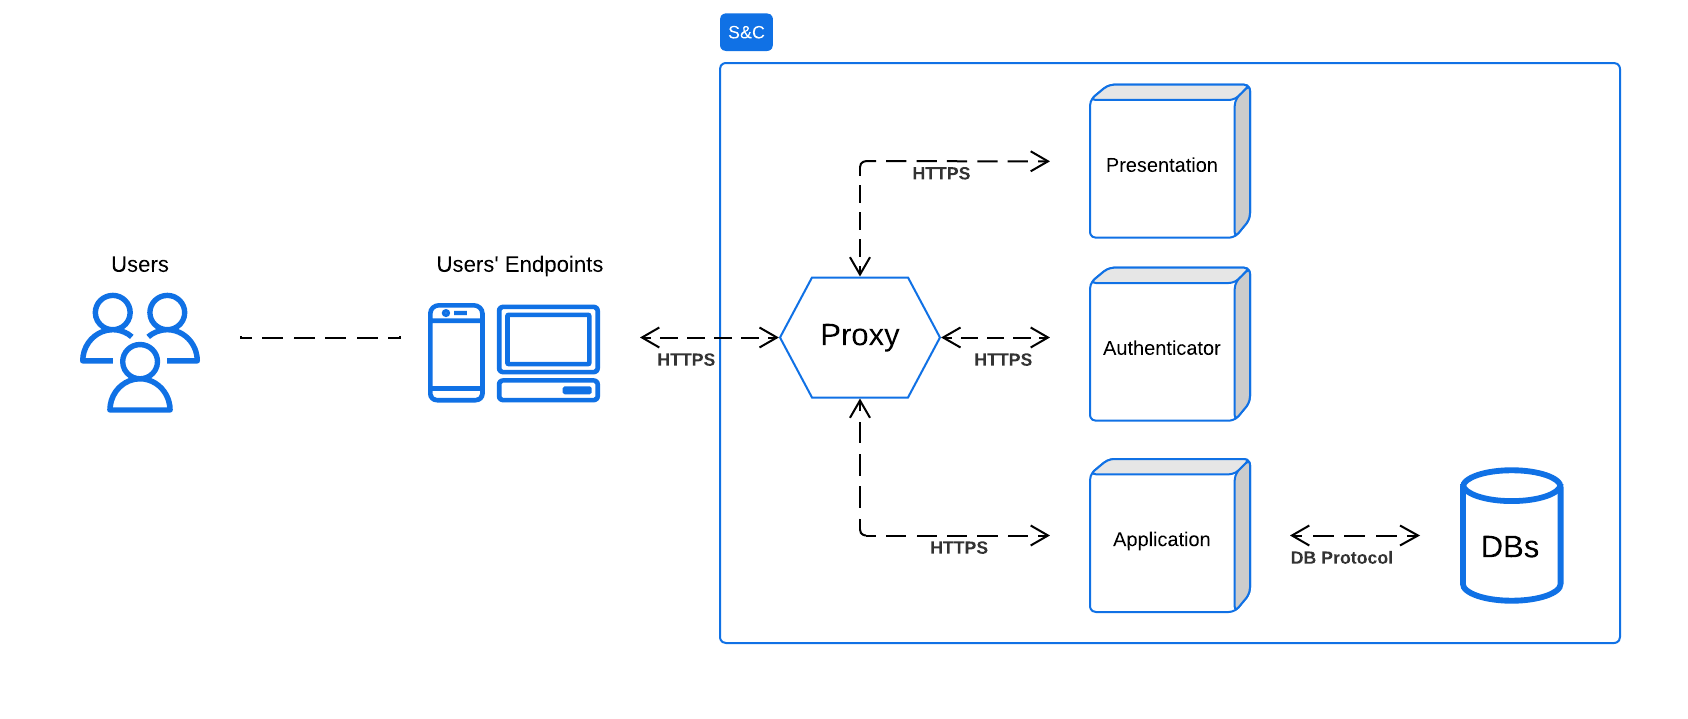
\includegraphics[width=\linewidth]{Latex/Images/DD/Overview0.png}
    \caption{Architectural Design Overview}
    \label{fig:ASoverview}
\end{figure}
\subsection{Component View}
This section provides a more in-depth view of the software components that are part of the designed architecture, as well as the necessary interfaces between them.
\begin{figure}[H]
    \centering
    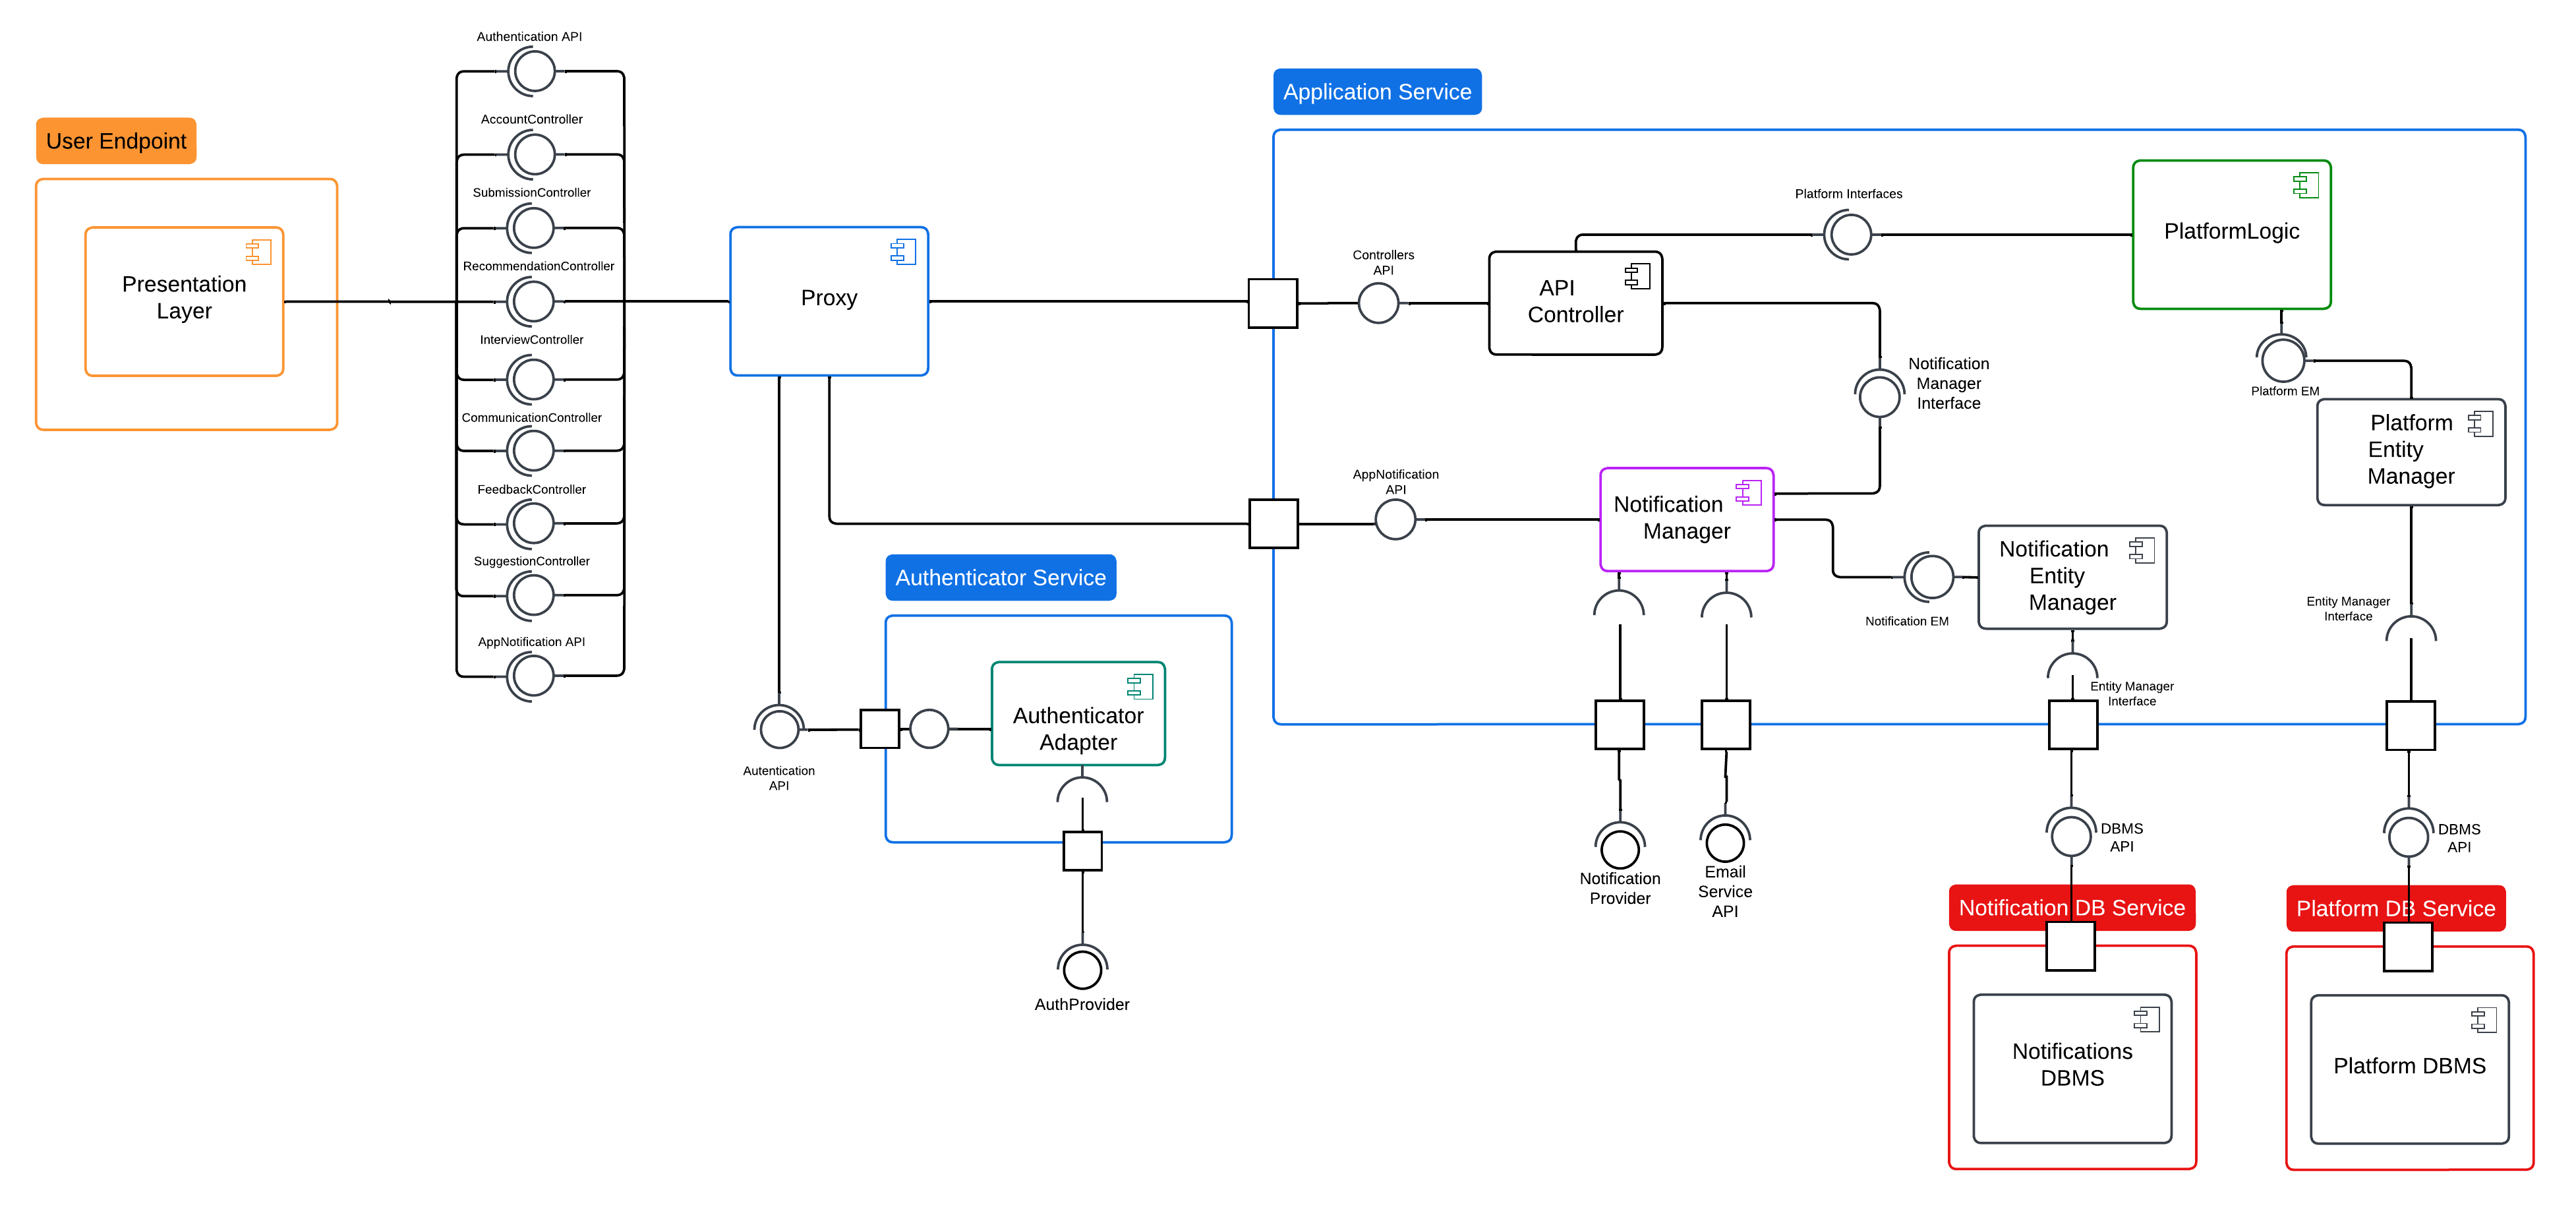
\includegraphics[width=\linewidth]{Latex/Images/DD/Component0.png}
    \caption{Architecture Components Diagram}
    \label{fig:Components}
\end{figure}
\subsubsection{Entity Manager}
The Entity Manager acts as an API that enables communication with a DBMS, simplifying ORM, querying, and data life cycles. It provides standard methods, independent of the specific DBMS used to handle the data. As shown in the diagram, there are two Entity Managers. The Platform Entity Manager provides its interface to the Platform Logic component, enabling interaction with the Platform DBMS. The Notification Entity Manager works analogously with the Notification DBMS.

\subsubsection{Platform Logic}
The inner components of the Platform Logic encapsulate the logic of the main parts of the S\&C environment. Each component autonomously handles its data management through the database, leveraging the Entity Manager interface.
\clearpage
\begin{figure}[H]
    \centering
    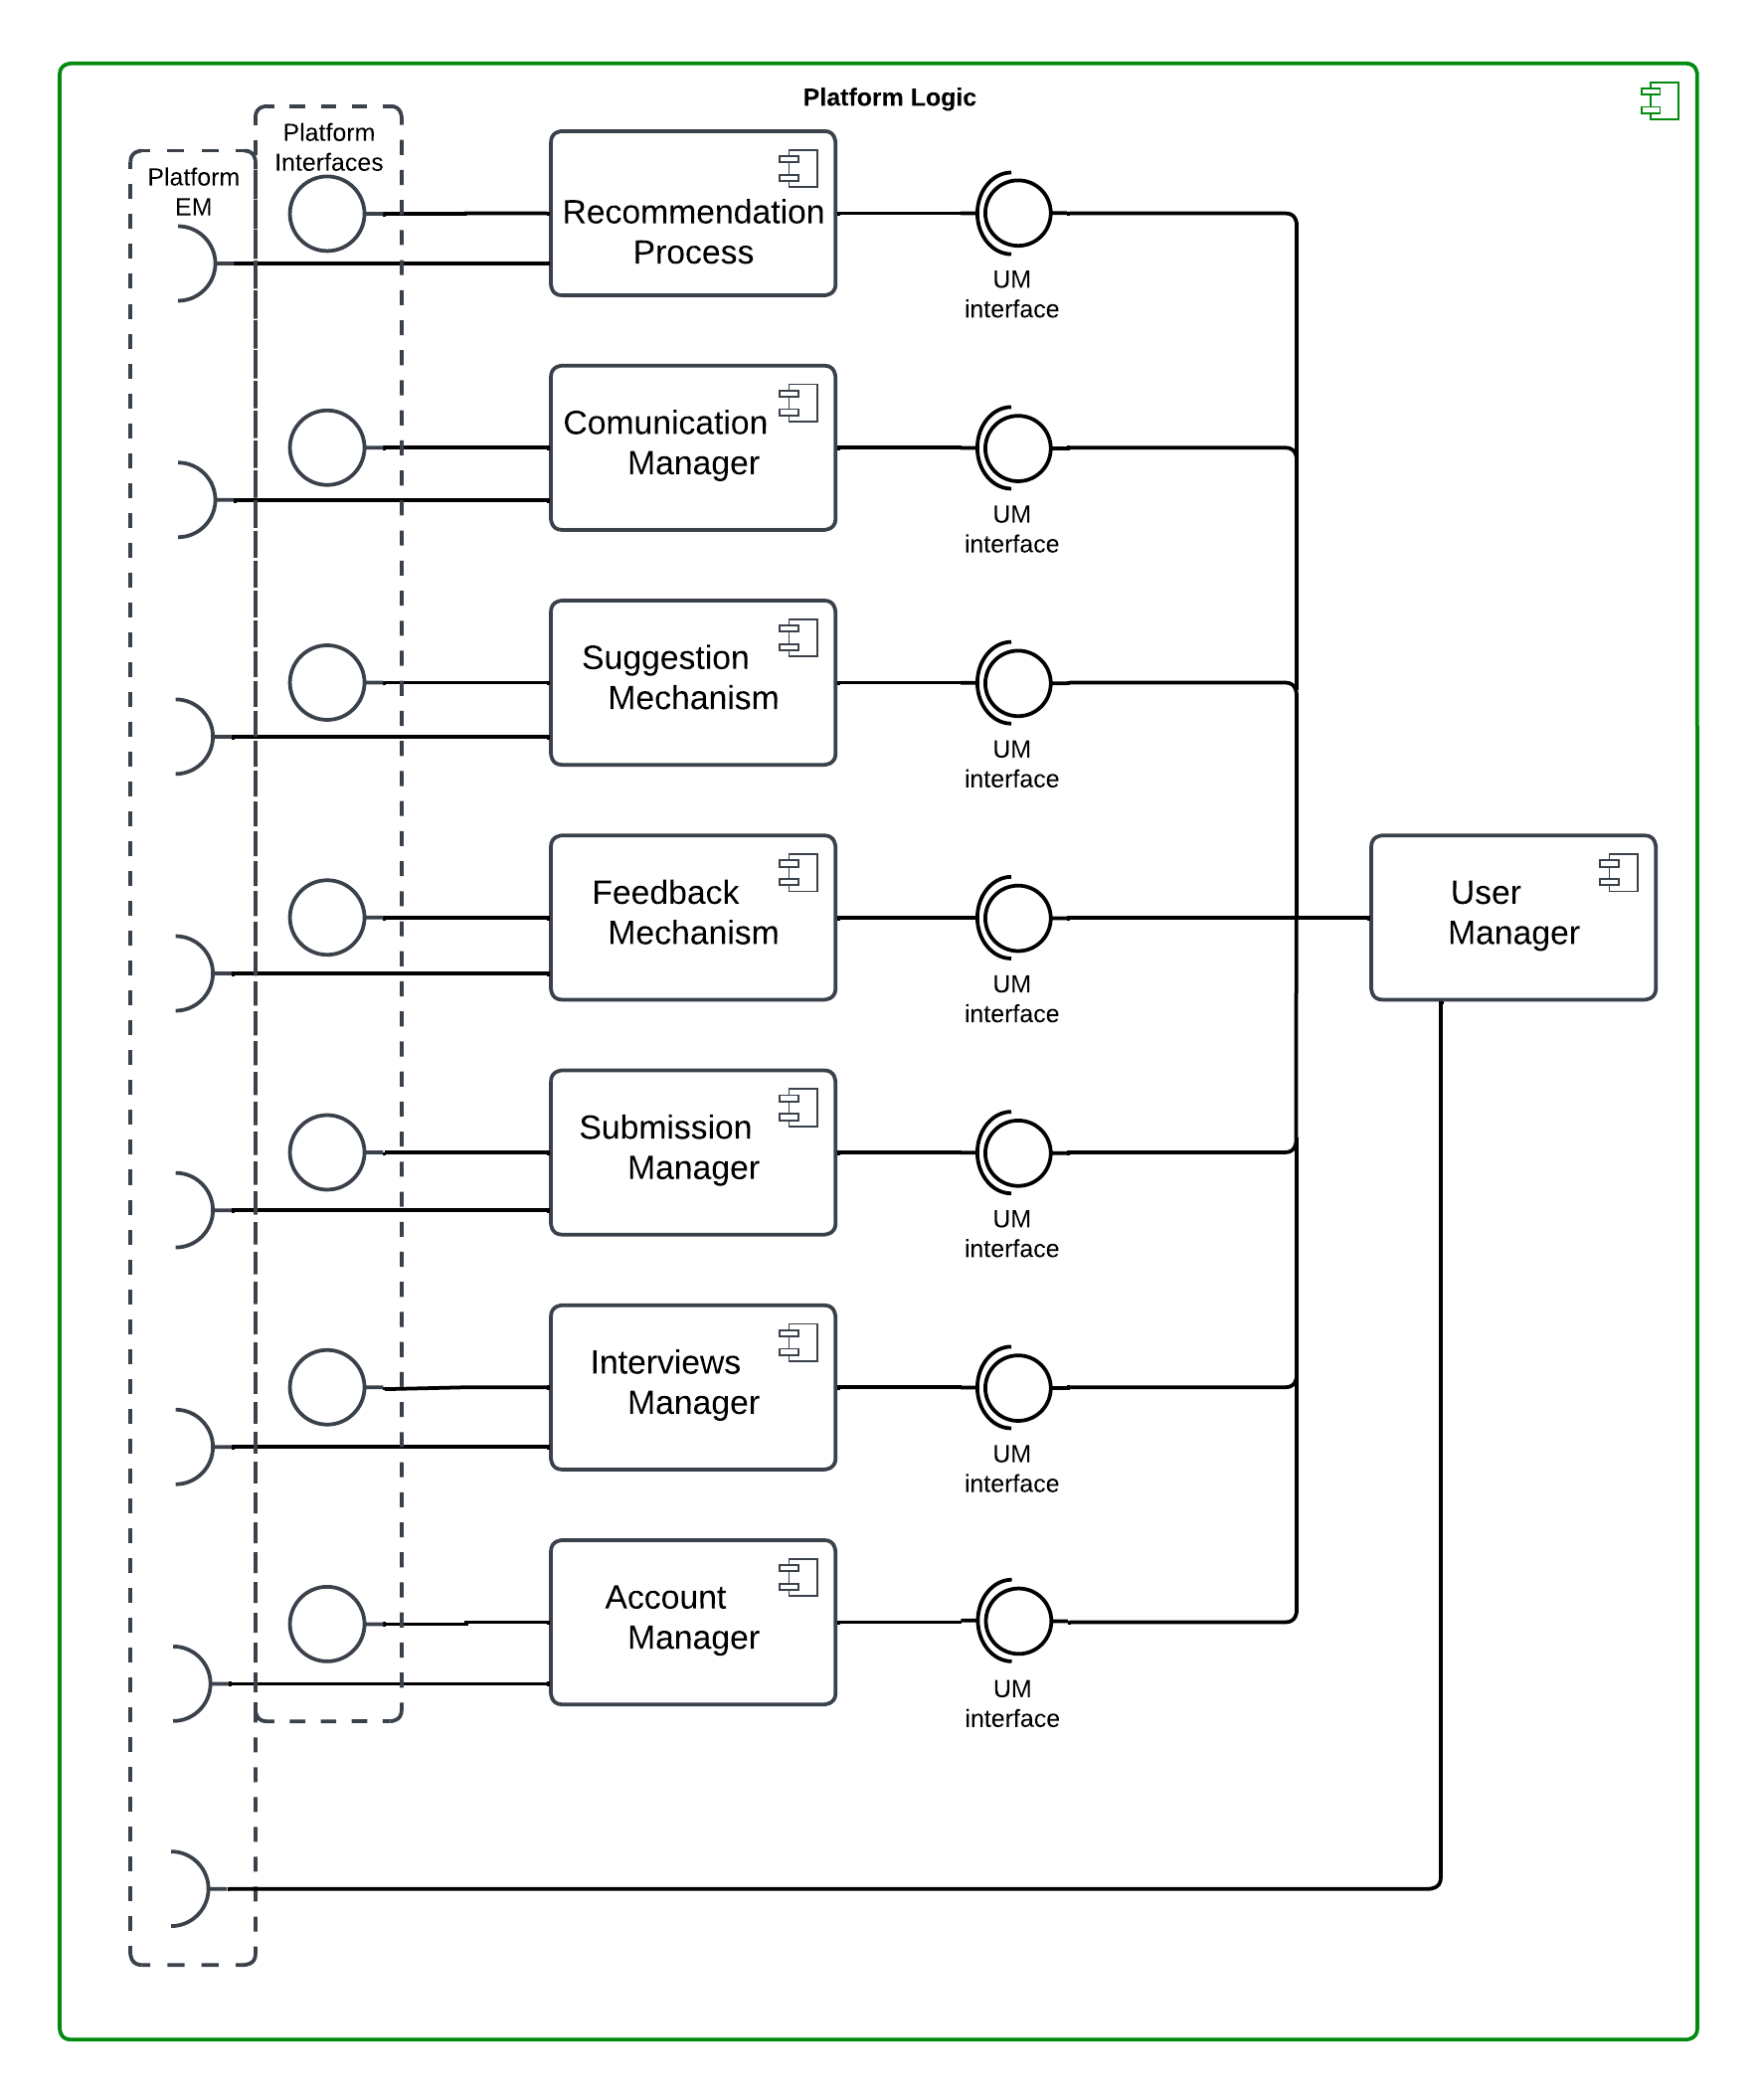
\includegraphics[width=0.8\linewidth]{Latex/Images/DD/Component1.png}
    \caption{Platform Logic Inner Components Diagram}
    \label{fig:PlatformComponents}
\end{figure}

\begin{table}[h!]
\centering
\begin{tabular}{|c|p{10cm}|}
\hline
\textbf{Component}          & \textbf{Description}                                        \\ \hline
Recommendation Process      & Handles recommendation logic and related data              \\ \hline
Communication Manager       & Manages communication logic and related data               \\ \hline
Suggestion Mechanism        & Handles suggestions logic and related data                 \\ \hline
Feedback Mechanism          & Processes feedback logic and related data                  \\ \hline
Submission Manager          & Manages submission logic and related data                  \\ \hline
Interview Manager           & Handles interview-related logic and data                   \\ \hline
Account Manager             & Manages account logic and related data                     \\ \hline
User Manager                & Interface for querying and modifying user groups with specific characteristics \\ \hline
\end{tabular}
\caption{Description of platform components.}
\label{tab:platform_components}
\end{table}


\subsubsection{API Controller}
The API Controller consists of a set of inner controllers whose methods, triggered by user calls, interact with and execute the logic of the Platform Logic inner components depicted above.

\subsubsection{Notification Manager}
This component handles all notification-related needs, regardless of their type. It functions as an adapter for external push notification providers and email services, offering an interface to seamlessly integrate these external features with other services. It also creates and manages corresponding in-app notifications, which can be fetched by users through a dedicated AppNotification API.

This component serves as a clear example of a service that could easily be exported to its own container in the future, for instance, by exposing its own RESTful API to the Platform Logic instead of using the current interface-based setup.


\begin{figure}[H]
    \centering
    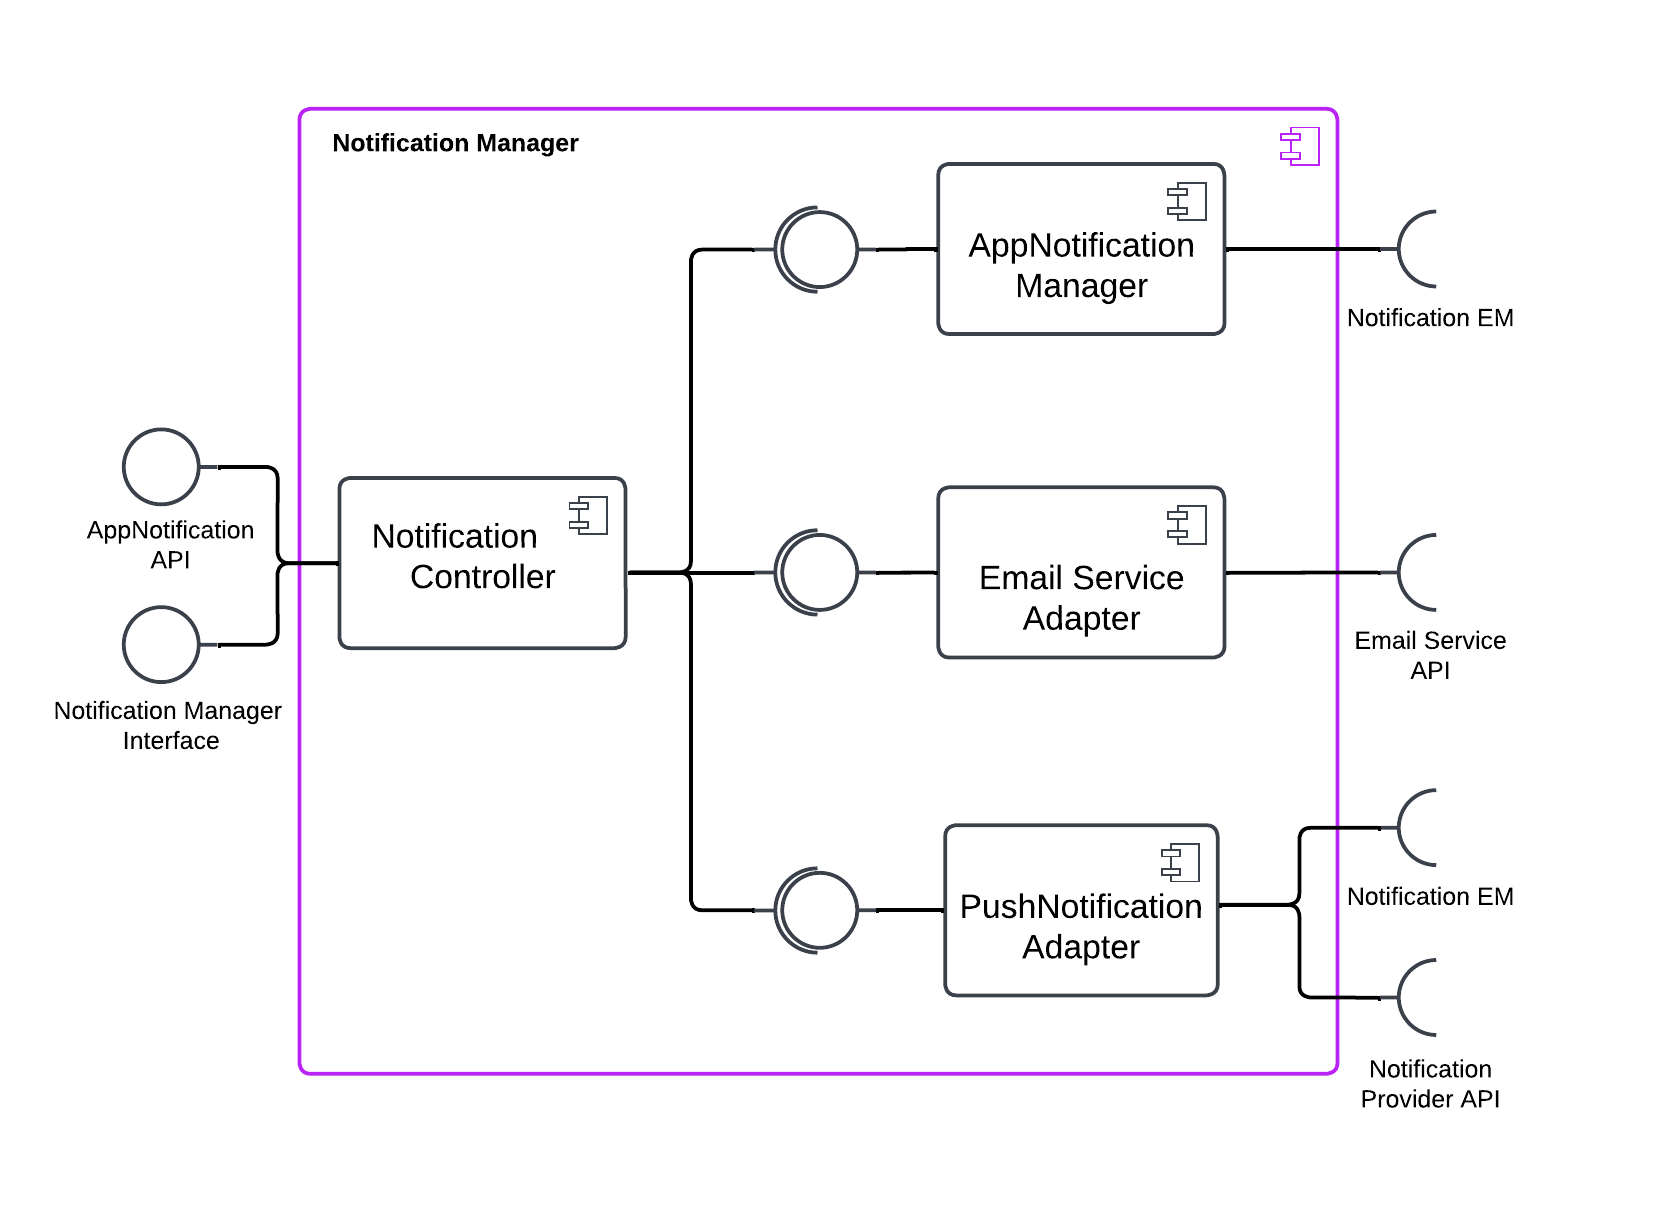
\includegraphics[width=0.8\linewidth]{Latex/Images/DD/Component2.png}
    \caption{Notification Manager Inner Components Diagram}
    \label{fig:NotificationComponents}
\end{figure}
\subsection{Deployment View}
Each service will be hosted on its own container being able to run independently on the same or on different machines. Containers, in addiction to make the development and deployment easier, also provide a good level of isolation and security.
The system will be hosted on the cloud and its container based nature allows to easily integrate orchestrator tools to decouple it from the cloud hosting provider and automatically manage scalability, reliability, fault tolerance and global security of the microservices cluster.
A DMZ can be implemented in this design by placing the Proxy in a dedicated network segment isolated from both the external network and the internal services. A firewall between the DMZ and the external network would allow only HTTP/HTTPS traffic to the Proxy, while another firewall between the DMZ and the internal network would restrict traffic to authorized services. This setup enhances security by exposing only the Proxy to external access, keeping all the other services, along with the databases, fully protected within the internal network.
\begin{figure}[H]
    \centering
    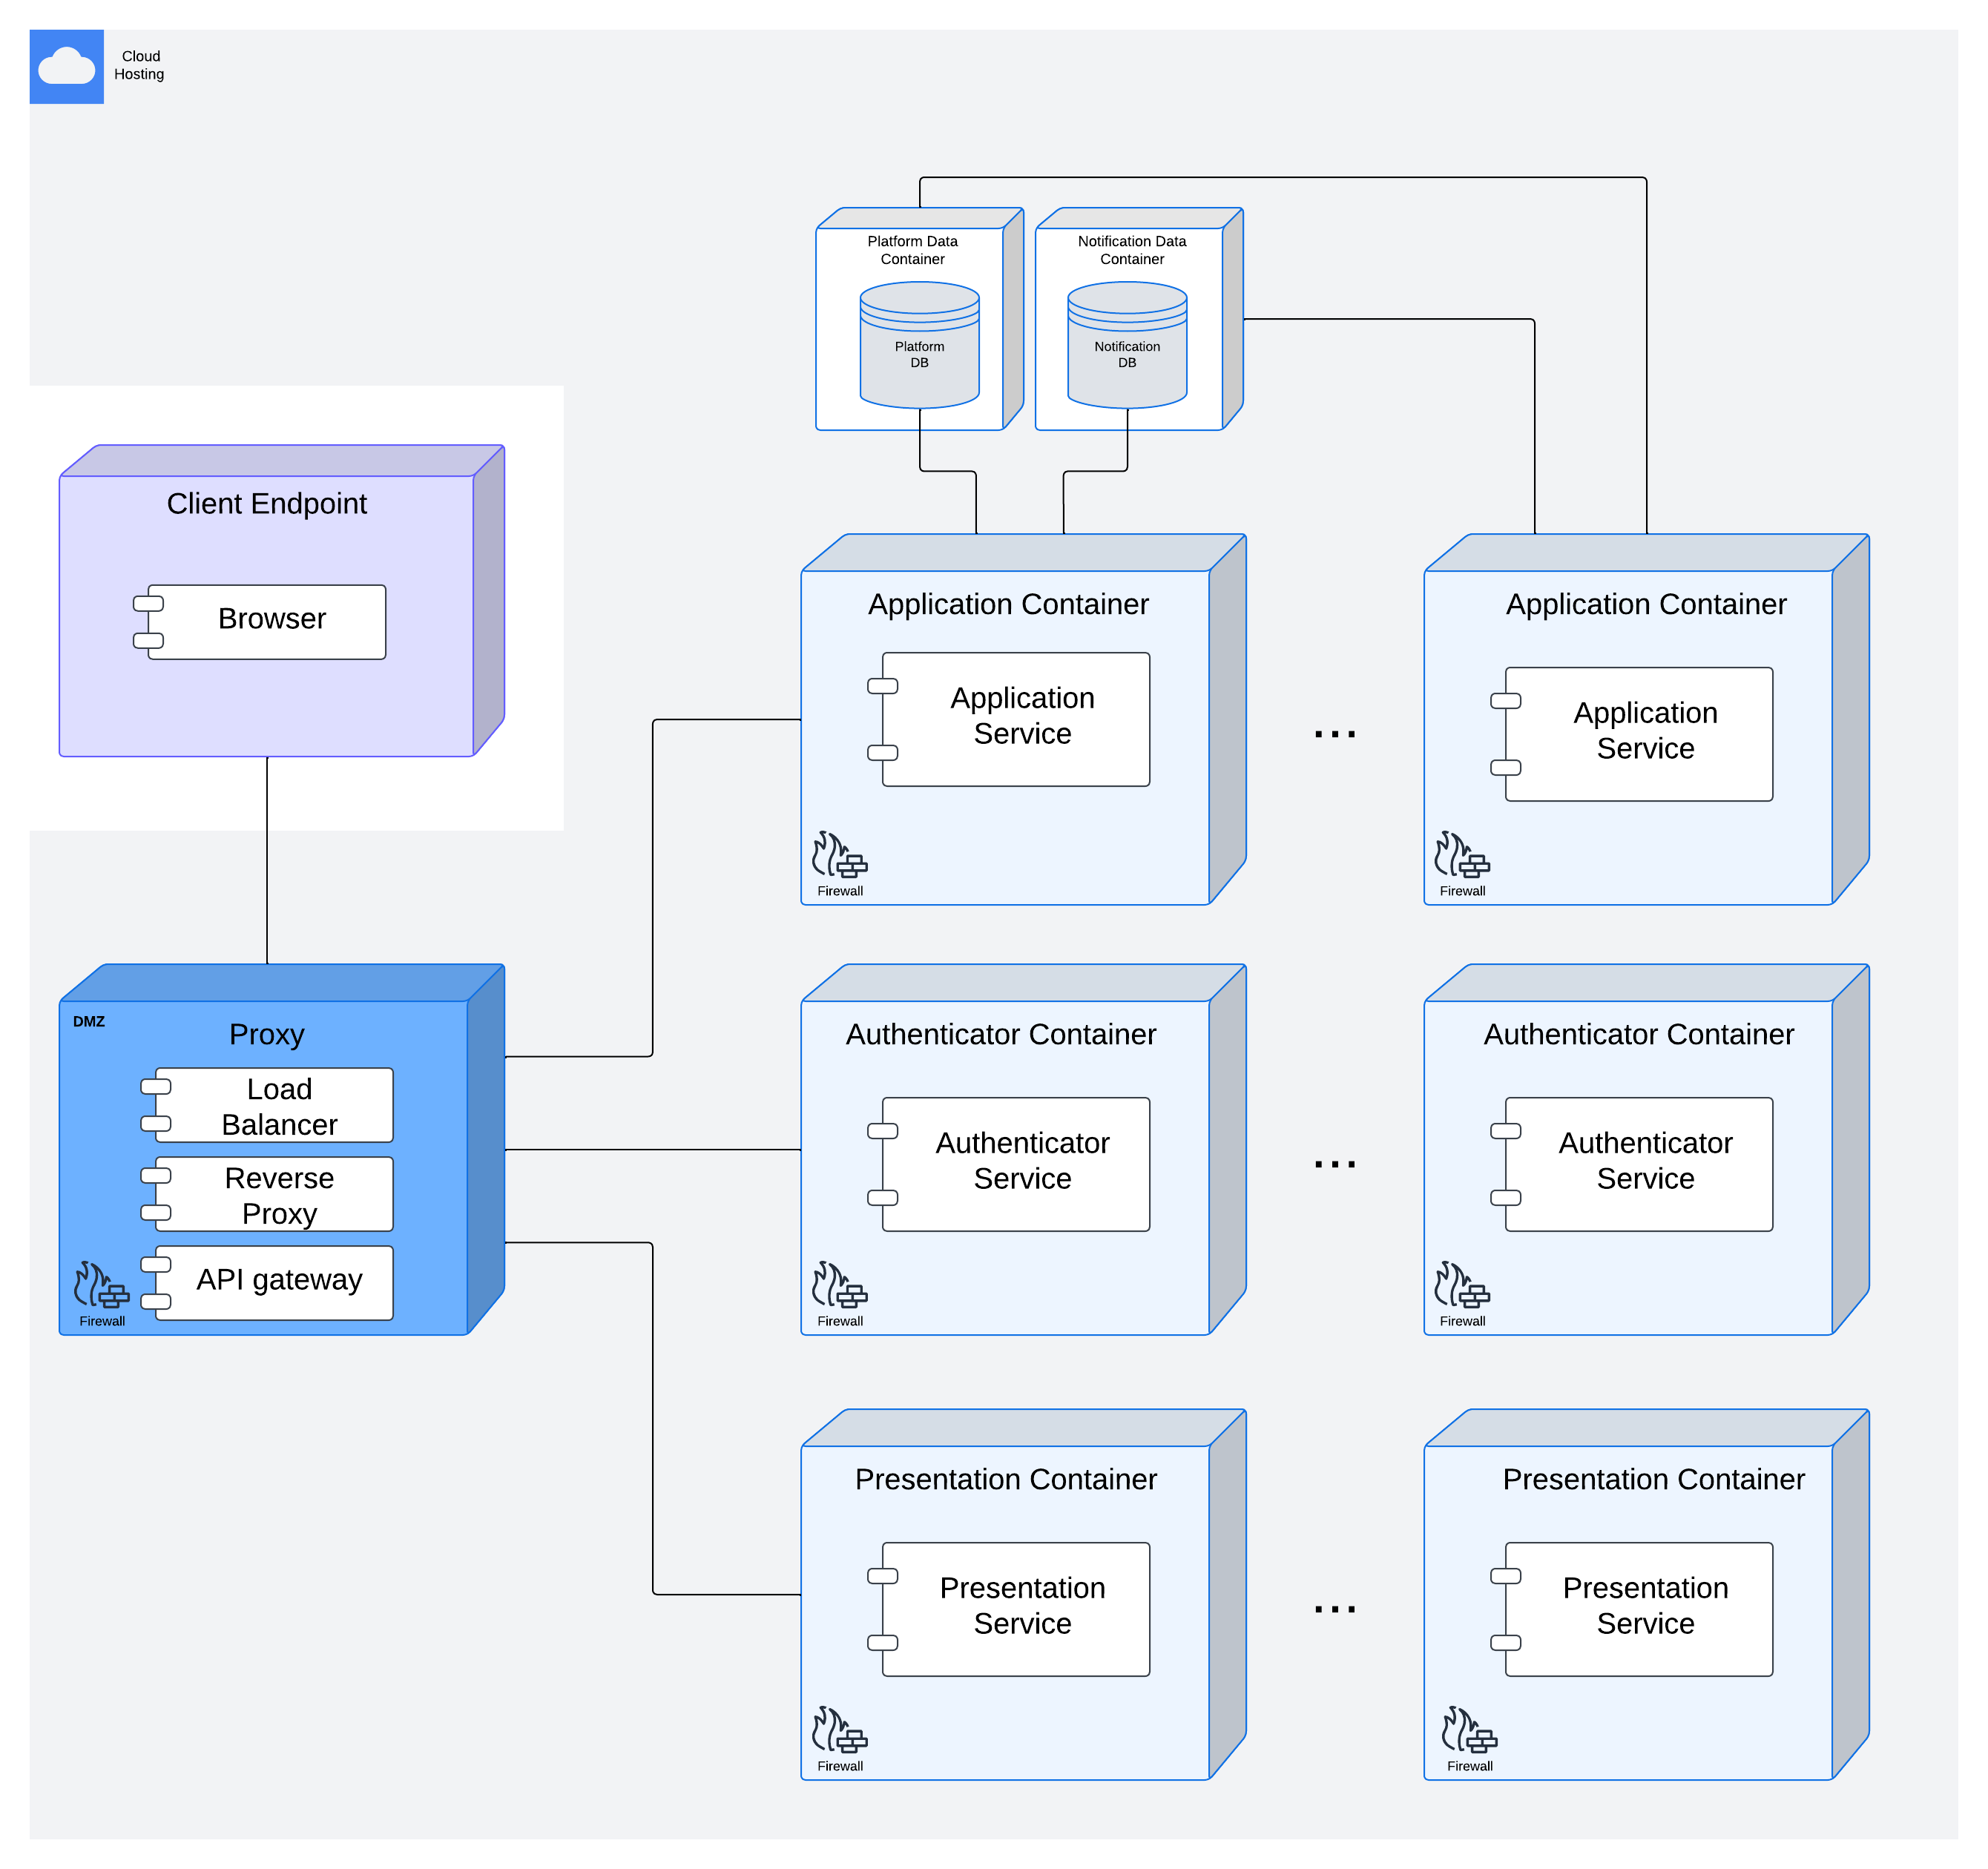
\includegraphics[width=0.8\linewidth]{Latex/Images/DD/Deployment.png}
    \caption{Deployment Diagram}
    \label{fig:Deployment}
\end{figure}
\subsection{Runtime View}
\subsubsection*{Sequence Diagrams Descriptions}

This section describes the interactions between system components during S\&C runtime, depicting their call stacks at a high level of abstraction. For this purpose, sequence diagrams will be used.

\noindent The call stacks are often similar, as they follow the patterns established in the previous sections. All calls are triggered by the user through the Presentation layer, which sends API calls to the Proxy. The Proxy, in turn, forwards the requests to the appropriate service and, depending on the request, may add a middleware API call before reaching the final target.

\noindent For API requests that need to pass data to the services, the data type—always a JSON object—is not directly specified in the arrow representing the API call but can be inferred from the parameters of the subsequent call stack methods.

\noindent By analyzing the API endpoints, the Proxy determines where to redirect the requests, triggering middleware procedures such as those for authentication. These procedures will be described in advance, as they form the foundation for understanding the diagrams presented later in the section.

\noindent Every database interaction is performed through Entity Managers, which are responsible for querying the respective DBMS. All the steps described in purple are explained in detail in different runtime views.

\noindent Before proceeding to other diagrams, it is highly recommended to review the UserRegistration and UserLogin diagrams, as they are the most complex and thoroughly described ones. The other diagrams are more intuitive and, for this reason, less detailed, as they should be easily understood after gaining a general understanding of the first two.

\noindent Representing every return code or message for each call would be confusing. However, since failure behaviors are often shared across components, we have distributed the possible alternatives among all the diagrams rather than including all possibilities in each one. Additionally, due to the system's complexity, we have chosen to represent the notification sending process as a single action performed by the Notification Manager, without detailing the actions of its internal components, which are fully shown in the component view. We also decided to simplify the DBMS response to a generic “result” when the query returns data, and a generic “success” when the query is successful but returns no data.

\subsubsection*{User Registration Diagram}

\begin{figure}[H]
    \centering
    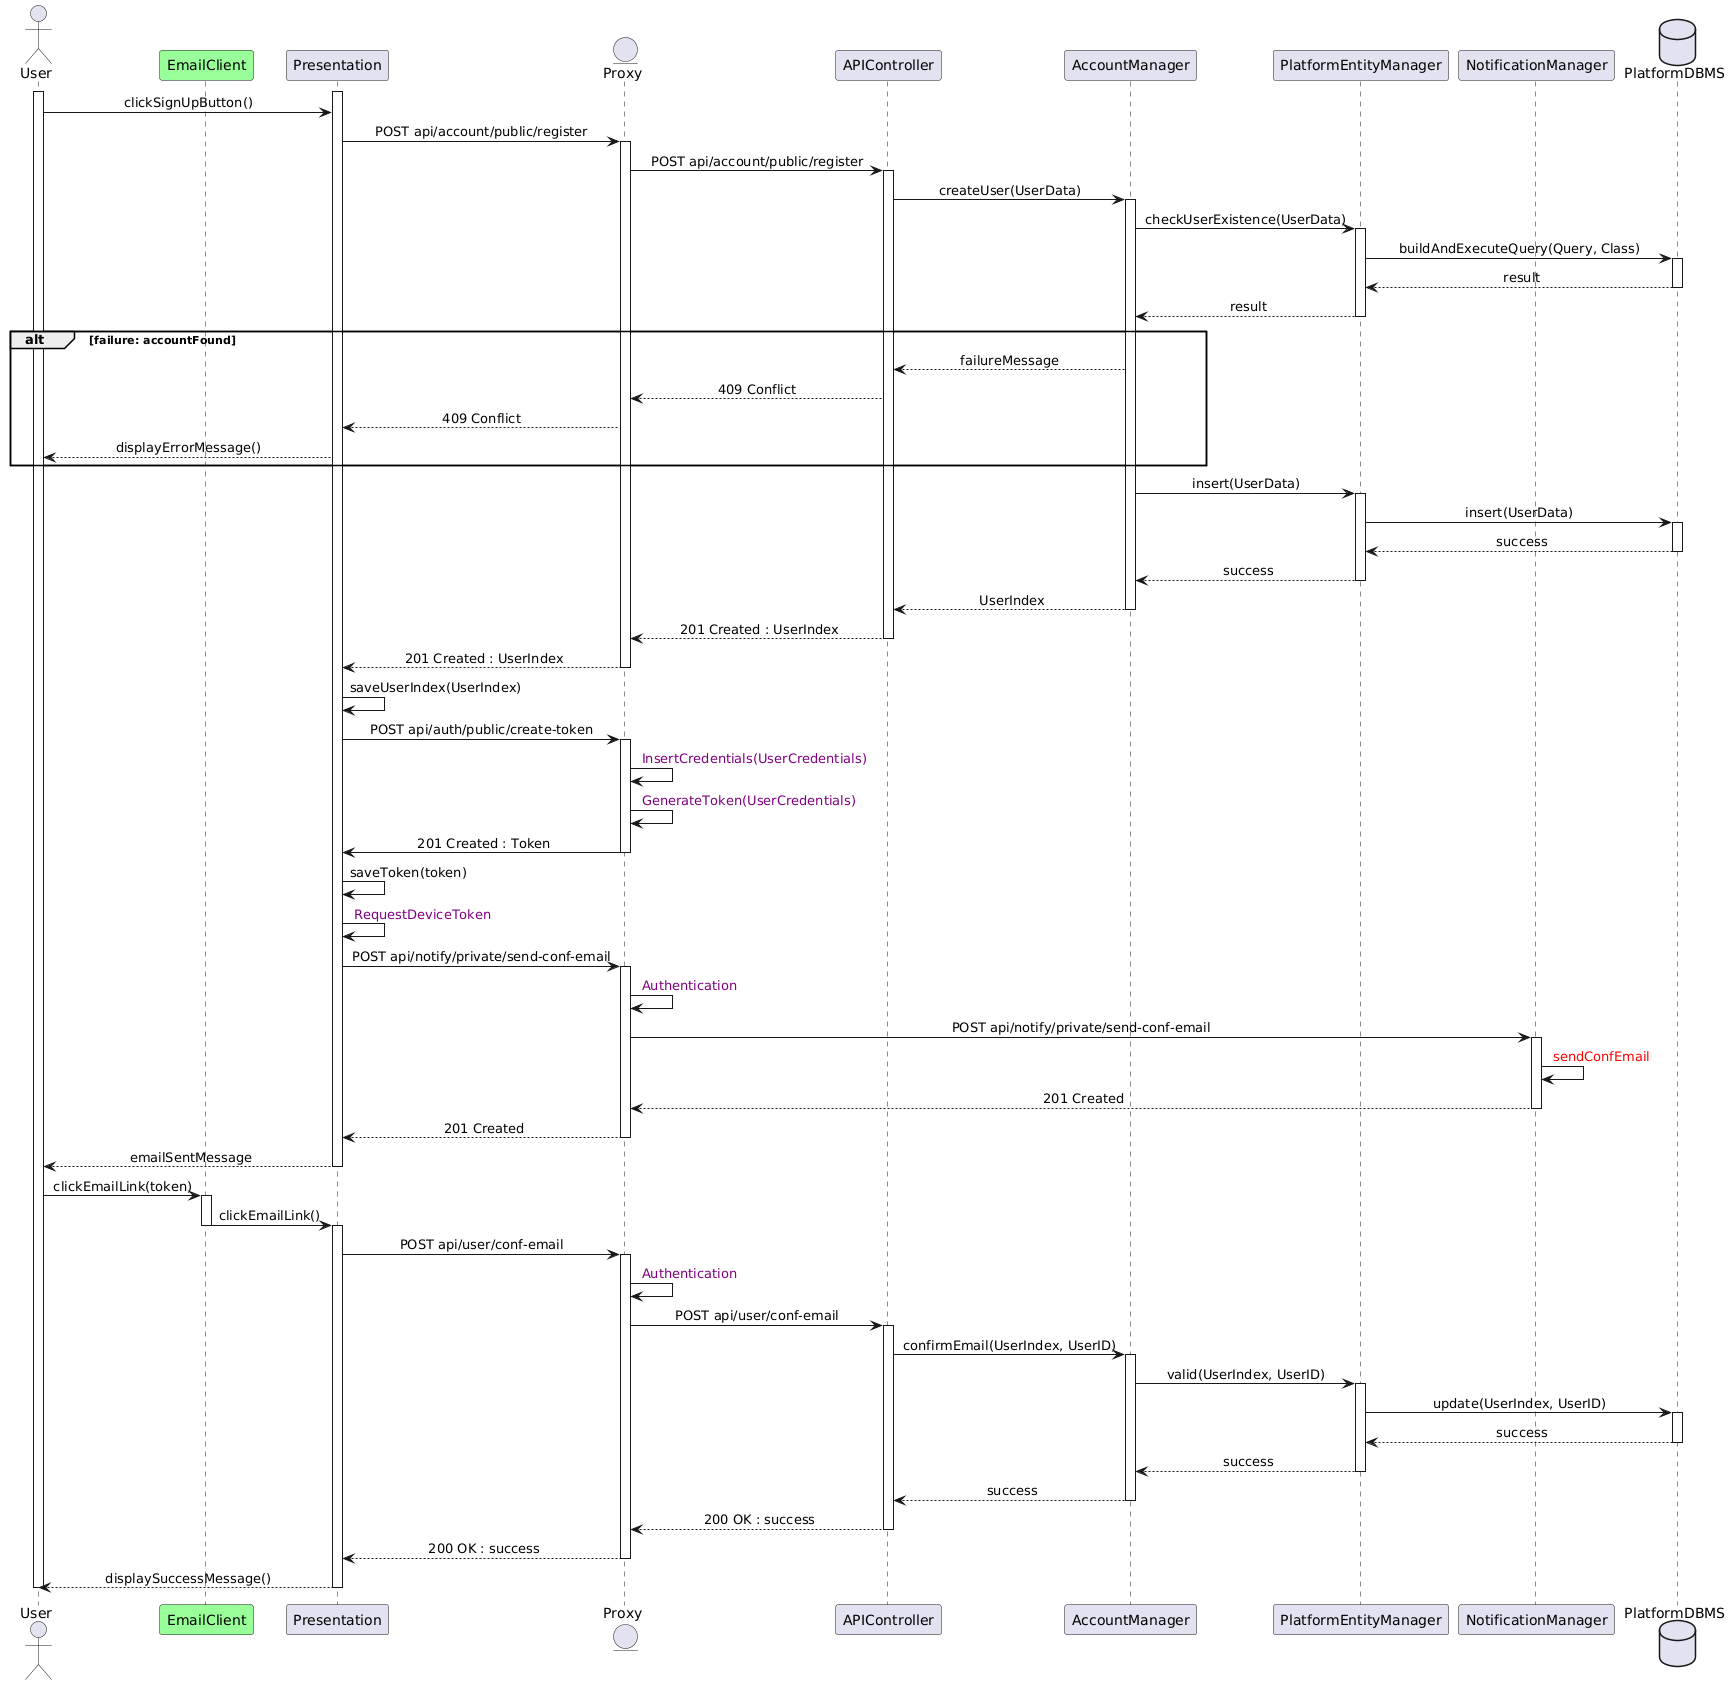
\includegraphics[width=\linewidth]{Latex/Images/DD/SequenceDiagrams/1.0UserRegistration.png}
    \caption{User Registration Sequence Diagram}
    \label{fig:userregistration}
\end{figure}

The User Registration view is the most complex one, as it involves the initial procedure for all the features of our web application, such as authentication, session validation, and notifications.\\
When the User clicks the SignUp Button, the Presentation Layer sends a POST request to the Proxy with the UserData object in its body. The Proxy recognizes the request as public based on the endpoint and forwards it to the Application Service's API Controller.\\
The API Controller accesses the AccountManager, which queries the databases through the Platform Entity Manager to check for user existence. If the User exists, the call stack proceeds backward, returning an error to the User. This could happen, for instance, if the user enters an email or a VAT that is already in use. If the UserData is unique and valid, the AccountManager creates a new User and stores it in the database.\\
A success API call code and a UserIndex object are returned to the Presentation Layer, which saves the object locally. The UserIndex is required to modify the UserData in the next step.\\
Then, the Presentation Layer sends a POST request with the UserCredential object to the Authenticator to generate the session token. The Proxy adds a middleware request to the Authenticator to insert the UserCredentials, a required step to allow the Authenticator to generate the token. For a detailed view see the \textit{(fig:\ref{fig:generatetoken}) InsertCredentials} and \textit{(fig:\ref{fig:generatetoken}) GenerateToken} diagrams\\
After the token is generated, the Authenticator returns it to the Presentation Layer, which saves it for future private calls. The Presentation Layer then sends a request to obtain a DeviceToken, which will be needed to notify its endpoint device. See for an in-depth view of the \textit{(fig:\ref{fig:requestdevicetoken}) RequestDeviceToken} step.\\
The final call triggered by the button click is a POST request responsible for sending the email confirmation. Since the request is to a private endpoint, the Proxy adds a middleware request to the Authenticator service to authenticate the user using the previously obtained token, provided in the header of every private API call. To understand how the Authentication works in detail, see the \textit{(fig:\ref{fig:authentication}) Authentication} diagram.\\
After validation, the Proxy forwards the request to the NotificationManager, which sends the email by communicating with the EmailServiceProvider. The communication with the EmailServiceProvider is not shown in the diagram to avoid unnecessary complexity, as it consists of a simple call to an external service. For this reason, it is depicted in red text.\\
The EmailServiceProvider sends the email to the User and returns a success message to the NotificationManager, which forwards it to the Presentation Layer, ultimately returning control to the User.\\
The User receives the email and clicks the link to confirm their email using their EmailClient. The EmailClient link opens a Presentation Layer page, which sends a POST request to the Proxy. The Proxy authenticates the user as described earlier and forwards the request to the Application Service's API Controller, which accesses the AccountManager to activate the User. The AccountManager updates the User's status in the database and returns a success message to the Presentation Layer, which displays it to the User.\\
The User is now successfully registered and can use the web application features.

\subsubsection*{InsertCredentials - GenerateToken}
\begin{figure}[H]
    \centering
    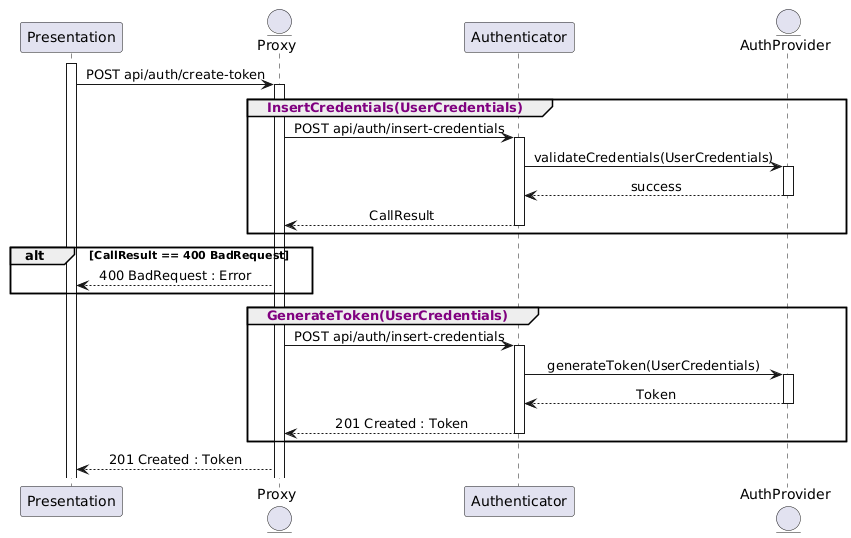
\includegraphics[width=\linewidth]{Latex/Images/DD/SequenceDiagrams/1.1InsertCredentialsGenerateToken.png}
    \caption{InsertCredentials - GenerateToken Sequence Diagram}
    \label{fig:generatetoken}
\end{figure}
By adding the InsertCredentials middleware call, the Proxy simply calls the POST method of the Authenticator service with the UserCredentials object in its body.
The Authenticator communicates with the external AuthProvider, which adds the UserCredentials to its database.\\
Every call to an external service provider can generate errors that do not depend on our system. These errors typically correspond to response codes starting with 5 - -  and should be handled properly.
However, there can also be errors that depend on our system, such as a malformed UserCredentials object. These errors typically have codes starting with 4 - -, and this type of error is depicted in the diagram as a failure example.\\
If the call is successful, the AuthProvider returns a success message to the Authenticator, which forwards it to the Proxy. The Proxy then proceeds with the GenerateToken step, which consists of a POST call to another Authenticator endpoint responsible for generating the token associated with the UserCredentials object.\\
The Authenticator communicates with the AuthProvider to generate the token and returns it to the Proxy. The Proxy forwards the token to the Presentation Layer, which saves it for future private calls, as shown in the previous diagram.

\subsubsection*{Authentication}
\begin{figure}[H]
    \centering
    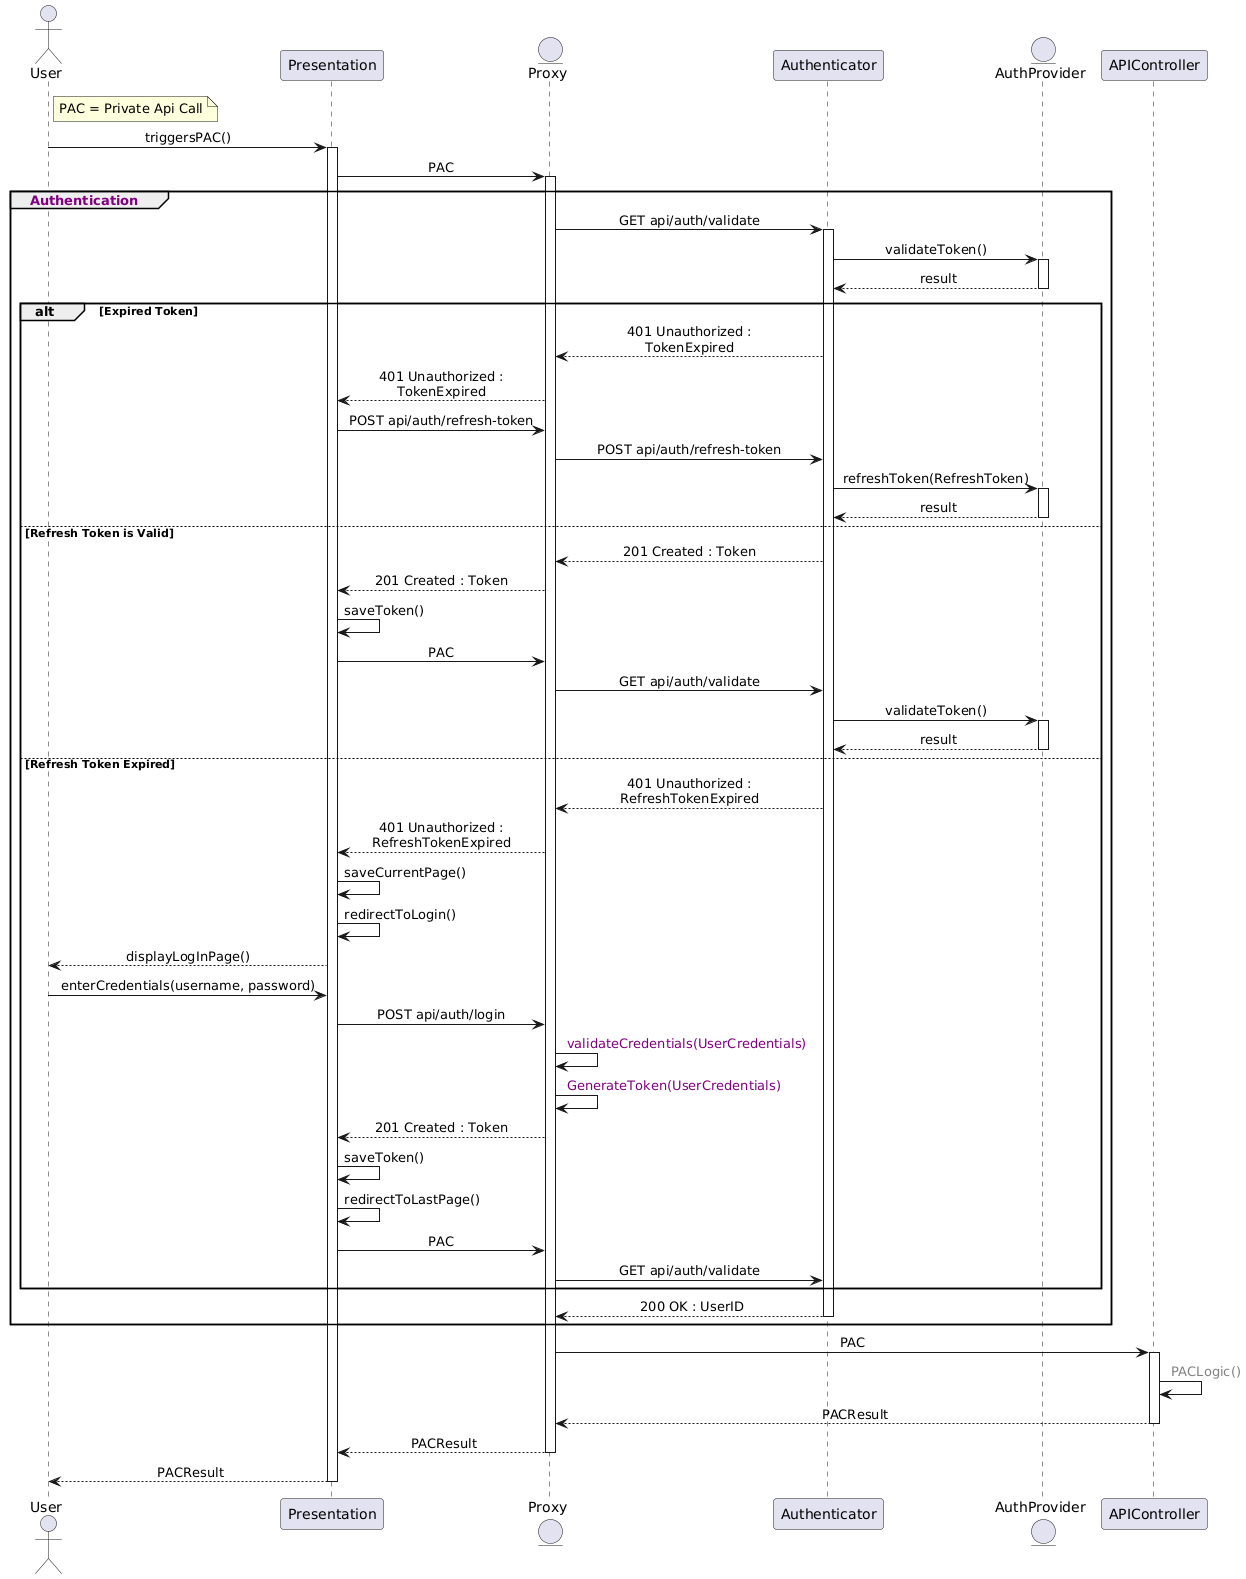
\includegraphics[width=\linewidth]{Latex/Images/DD/SequenceDiagrams/1.2Authentication.png}
    \caption{Authentication Sequence Diagram}
    \label{fig:authentication}
\end{figure}
When a private request is sent to the Proxy by the Presentation Layer, the Proxy adds a middleware call to the Authenticator to authenticate the user. The Authenticator receives a GET request and checks the token in the header.\\
If the token is valid, the Authenticator returns a success message to the Proxy, which forwards the request to the Application service.
If the token is invalid, the Authenticator returns an error message to the Proxy, which then forwards the error message to the Presentation Layer.\\
The Presentation Layer first attempts to refresh the token using the RefreshToken provided when the authentication token was originally issued.
If the RefreshToken is valid, the Presentation Layer will request a new token from the Authenticator.
If the RefreshToken is also invalid, the Presentation Layer will save the current page and redirect the user to the login page to re-authenticate and obtain a new authentication token and RefreshToken.\\
After the UserLogin process is completed, the Presentation Layer will save the newly obtained token and redirect the user to the previously saved page.\\
For more details about the ValidateCredentials step, see the UserLogin diagram.

\subsubsection*{RequestDeviceToken}
\begin{figure}[H]
    \centering
    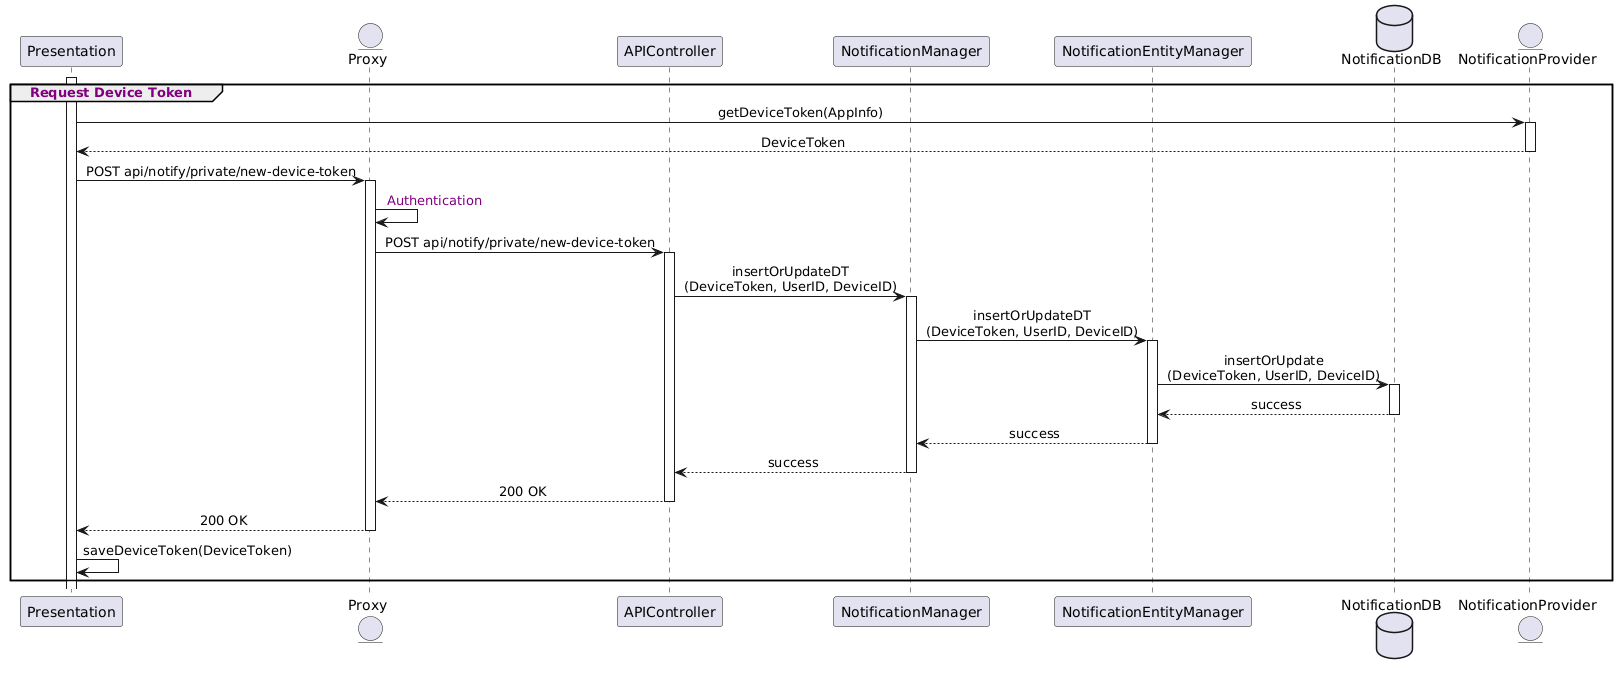
\includegraphics[width=\linewidth]{Latex/Images/DD/SequenceDiagrams/1.3RequestDeviceToken.png}
    \caption{RequestDeviceToken Sequence Diagram}
    \label{fig:requestdevicetoken}
\end{figure}
The RequestDeviceToken step begins with the Presentation Layer directly communicating with the NotificationProvider, which is responsible for handling the token associated with the user's endpoint device.\\
To obtain the DeviceToken, some device information—retrievable through browser methods—is sent to the external service provider. The NotificationProvider returns the DeviceToken to the Presentation Layer, which sends it to the Application service so that the NotificationManager can store it in its database and bind it to the User.\\
Since a user can access S\&C on multiple devices, a DeviceID object is required to inform the server which device the token is associated with. As a consequence, each device has its own DeviceToken, and a user can have multiple DeviceTokens, each bound to a unique DeviceID.\\
After the NotificationManager has stored the DeviceToken, it returns a success message to the Presentation Layer, which saves it locally.\\
The DeviceToken can expire or be invalidated by the external service provider. In that case is the Presentation Layer the one responsible to update the DeviceToken as shown next.

\subsubsection*{CheckDeviceToken}
\begin{figure}[H]
    \centering
    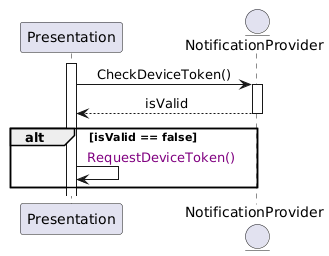
\includegraphics[width=0.5\linewidth]{Latex/Images/DD/SequenceDiagrams/1.4CheckDeviceToken.png}
    \caption{CheckDeviceToken Sequence Diagram}
    \label{fig:checkdevicetoken}
\end{figure}
The CheckDeviceToken step is scheduled by the Presentation Layer. It consist of a direct communication to the NotificationProvider to check the actual locally saved token. If the token is invalid, the Presentation Layer will request a new one as shown in the RequestDeviceToken step. If the token is valid, the Presentation Layer will do nothing.

\subsubsection*{UserLogin - ValidateCredentials}
\begin{figure}[H]
    \centering
    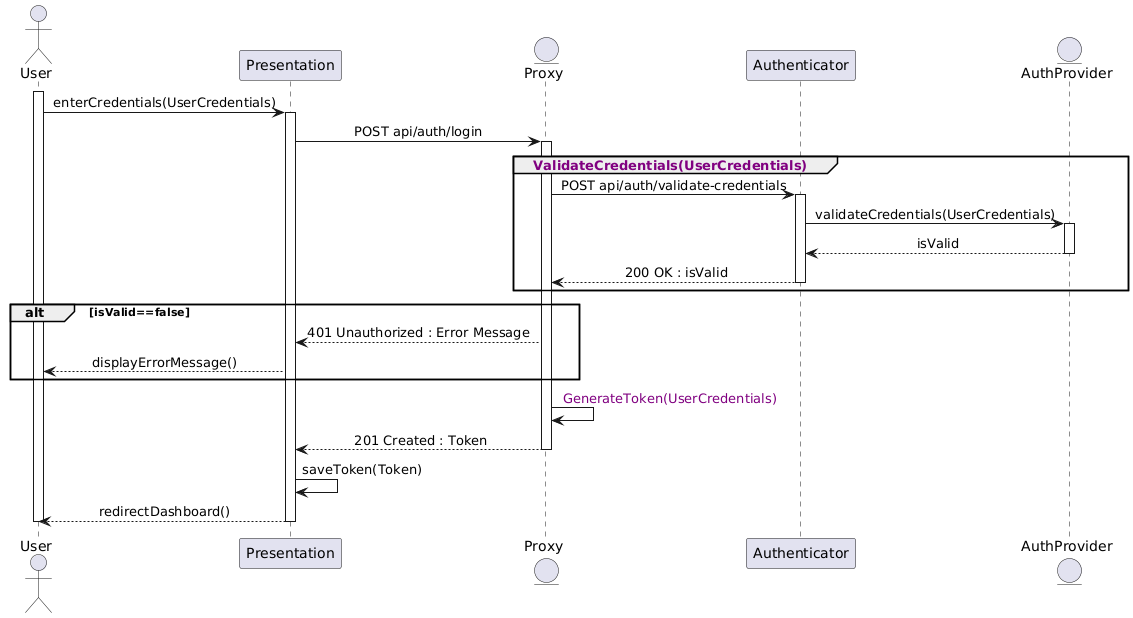
\includegraphics[width=\linewidth]{Latex/Images/DD/SequenceDiagrams/2UserLoginValidateCredentials.png}
    \caption{UserLogin ValidateCredentials Sequence Diagram}
    \label{fig:userlogin}
\end{figure}
By clicking the LogIn button, the user sends the entered UserCredentials from the Presentation Layer to the Proxy. This triggers a POST public request that reaches the Proxy. The Proxy adds a middleware call to the Authenticator to validate the UserCredentials. The Authenticator receives the request and checks the credentials in the AuthProvider. If the credentials are valid, the Proxy forwards the request again to the Authenticator, which generates the token associated with the provided credentials. The ValidateCredentials process differs from the InsertCredentials process because, for validation to succeed, the credentials must have been previously "inserted" into the AuthProvider. Once the token is generated, the Authenticator returns it to the Presentation Layer, which saves it for future private calls.

\subsubsection*{Participant Submission}
\begin{figure}[H]
    \centering
    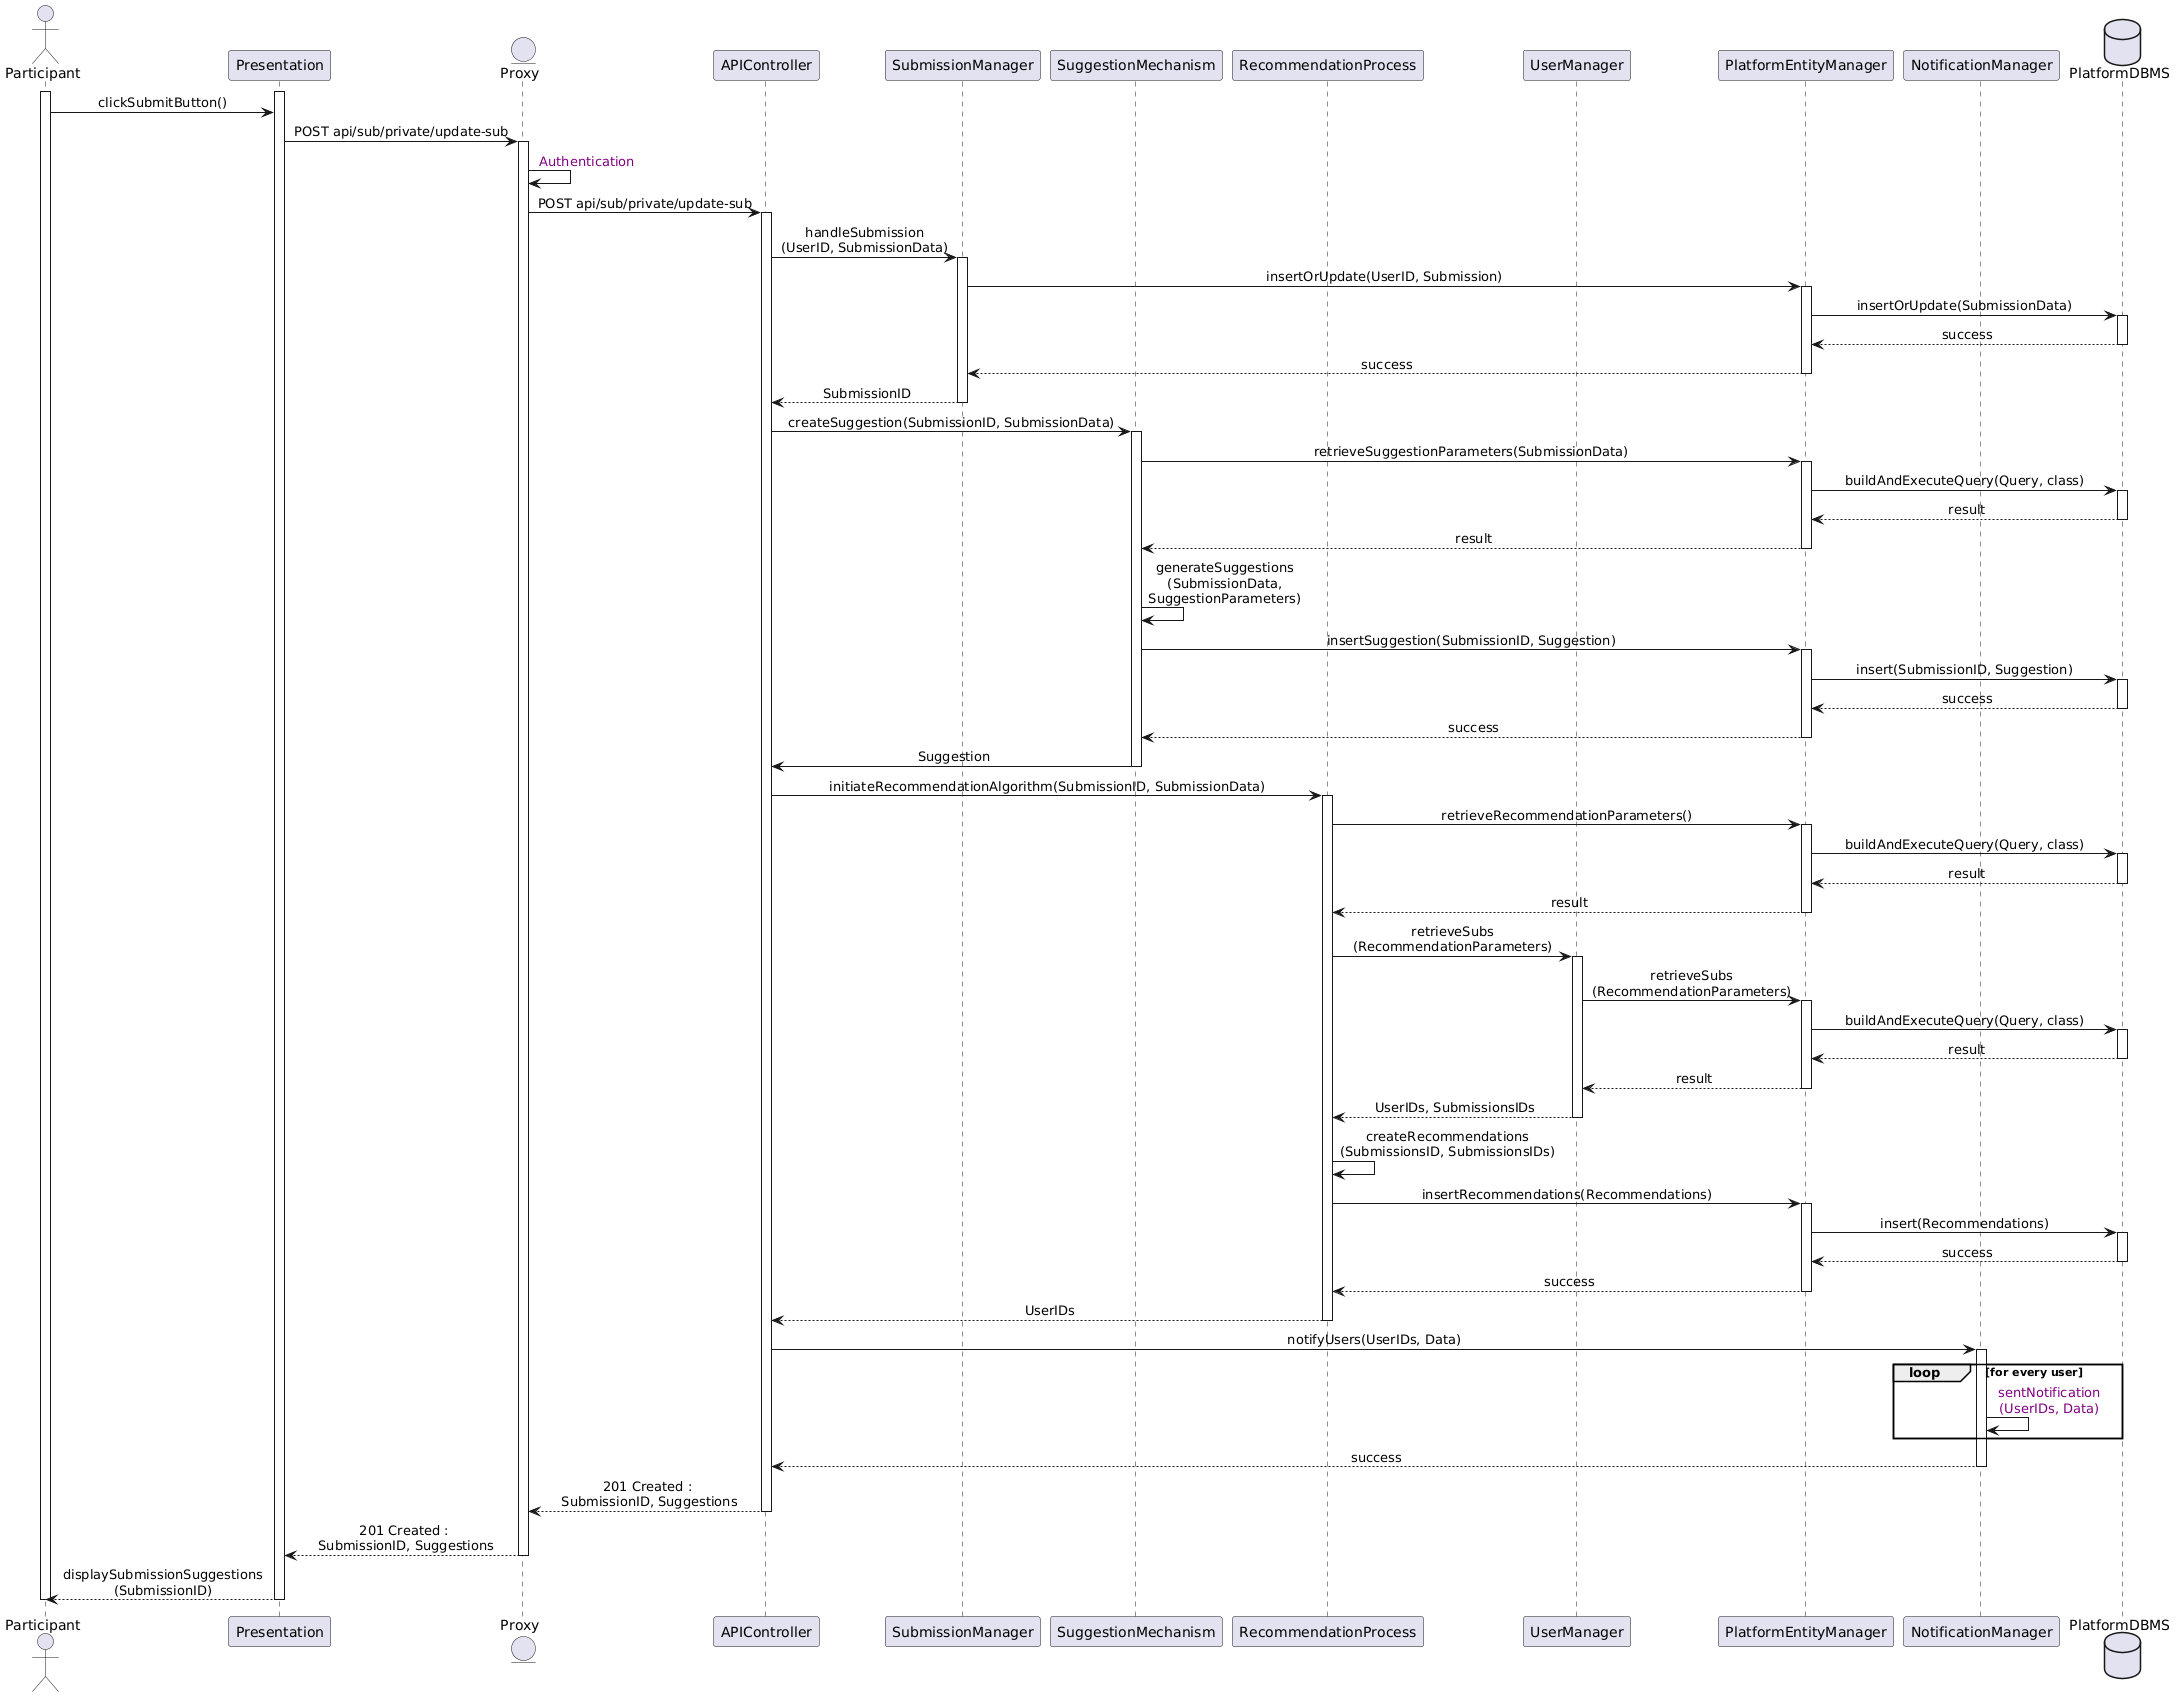
\includegraphics[width=\linewidth]{Latex/Images/DD/SequenceDiagrams/3ParticipantSubmission.png}
    \caption{Participant Submissions Sequence Diagram}
    \label{fig:participantsubmission}
\end{figure}
By clicking the Submit button, the Participant sends the submission data from the Presentation Layer to the Proxy. The triggered call is a POST private request, which the Proxy authenticates using the Authenticator. Once authenticated, the Proxy forwards the request to the APIController.\\
The APIController processes the submission by calling the SubmissionManager, which updates or inserts the data into the PlatformDBMS through the PlatformEntityManager. Afterward, the SuggestionMechanism generates suggestions for the submission, querying and updating the database as needed.\\
The APIController then triggers the RecommendationProcess, which identifies relevant users and submissions through the UserManager. Recommendations are generated, stored, and passed back to the APIController.\\
Finally, the NotificationManager notifies the identified users, and the APIController returns the SubmissionID and suggestions to the Presentation Layer, which displays them to the Participant.

\subsubsection*{Send Notification}
\begin{figure}[H]
    \centering
    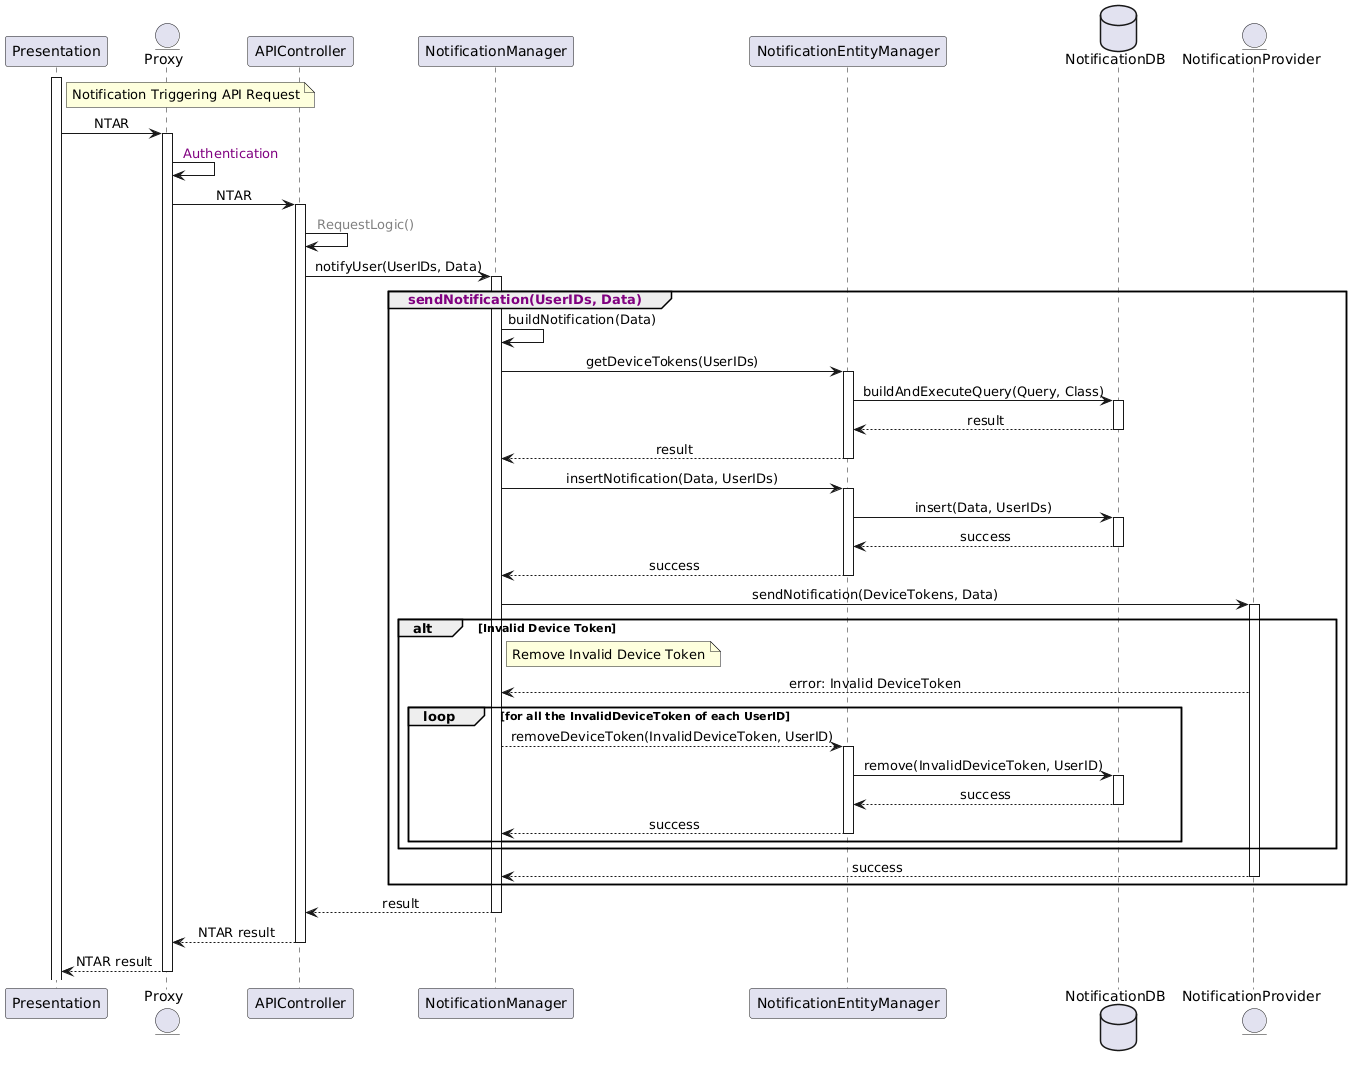
\includegraphics[width=\linewidth]{Latex/Images/DD/SequenceDiagrams/3.1SendNotification.png}
    \caption{Send Notification Sequence Diagram}
    \label{fig:sendnotification}
\end{figure}
The process begins when the Presentation Layer triggers a Notification Triggering API Request (NTAR) to the Proxy. The Proxy authenticates the request and forwards it to the APIController.\\
The APIController processes the request with the required logic and calls the NotificationManager to notify the specified users. The NotificationManager first builds the notification data and retrieves the device tokens of the users from the NotificationDB through the NotificationEntityManager.\\
After retrieving the device tokens, the NotificationManager stores the notification data in the NotificationDB and sends the notifications to the users' devices via the NotificationProvider.\\
If any invalid device tokens are detected during this process, the NotificationProvider returns an error, prompting the NotificationManager to remove these invalid tokens from the NotificationDB for each associated user.\\
Once the notifications are successfully sent, or all invalid tokens are handled, the NotificationManager returns the result to the APIController. The APIController forwards the result back to the Proxy, which then returns it to the Presentation Layer.\\
Note that the NotificationManager simply removes the invalid tokens from the NotificationDB. Is the Presentation Layer the one responsible to update the DeviceToken as shown in the CheckDeviceToken step.

\subsubsection*{User Opens Company Internship Offer}
\begin{figure}[H]
    \centering
    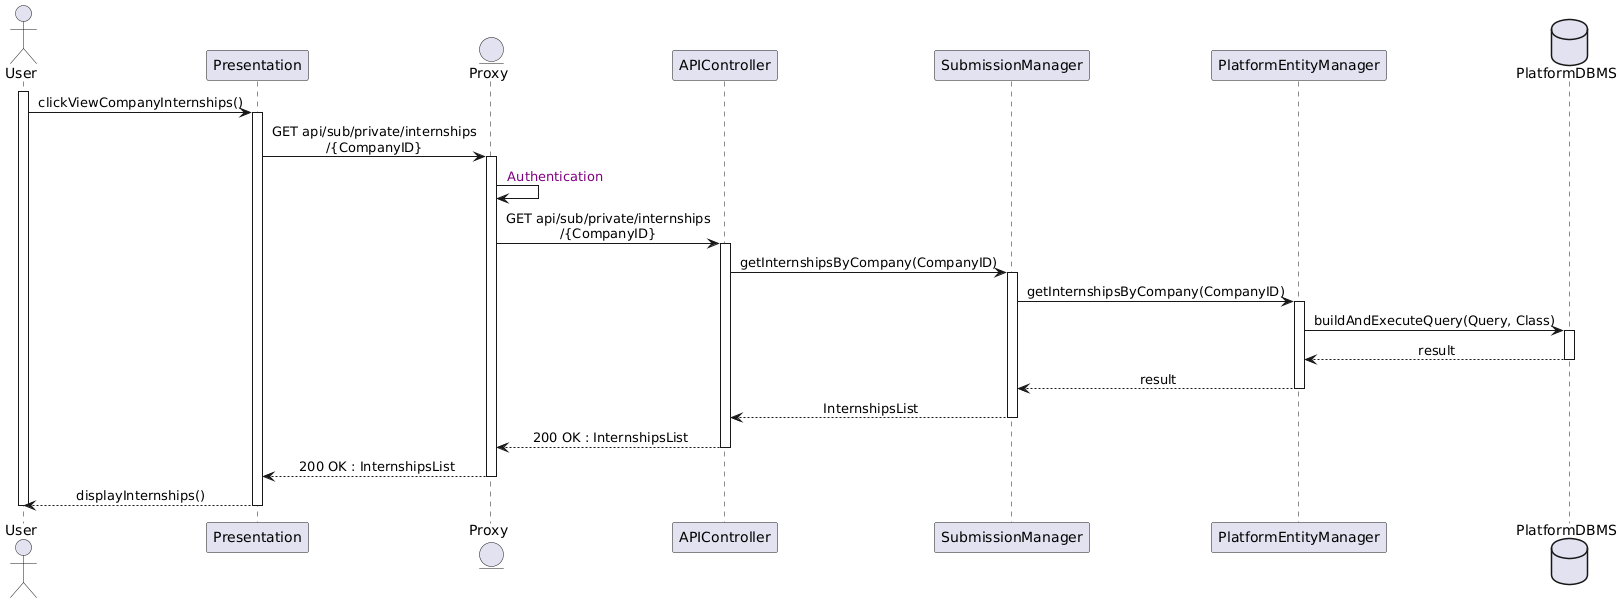
\includegraphics[width=\linewidth]{Latex/Images/DD/SequenceDiagrams/4UserOpensCompanyIntOffer.png}
    \caption{User Opens Company Internship Offer Sequence Diagram}
    \label{fig:useropensintoff}
\end{figure}
By clicking the View Company Internships button, the User triggers a GET private request from the Presentation Layer to the Proxy. The Proxy authenticates the request using the Authenticator and forwards it to the APIController in the Application Service.\\
The APIController calls the SubmissionManager to retrieve the internships associated with the specified CompanyID. The SubmissionManager queries the database via the PlatformEntityManager, which executes the query in the PlatformDBMS and returns the results.\\
The SubmissionManager sends the list of internships back to the APIController, which forwards it to the Proxy. The Proxy then returns the response to the Presentation Layer, which displays the internships to the User.

\subsubsection*{User Opens Student CV}
\begin{figure}[H]
    \centering
    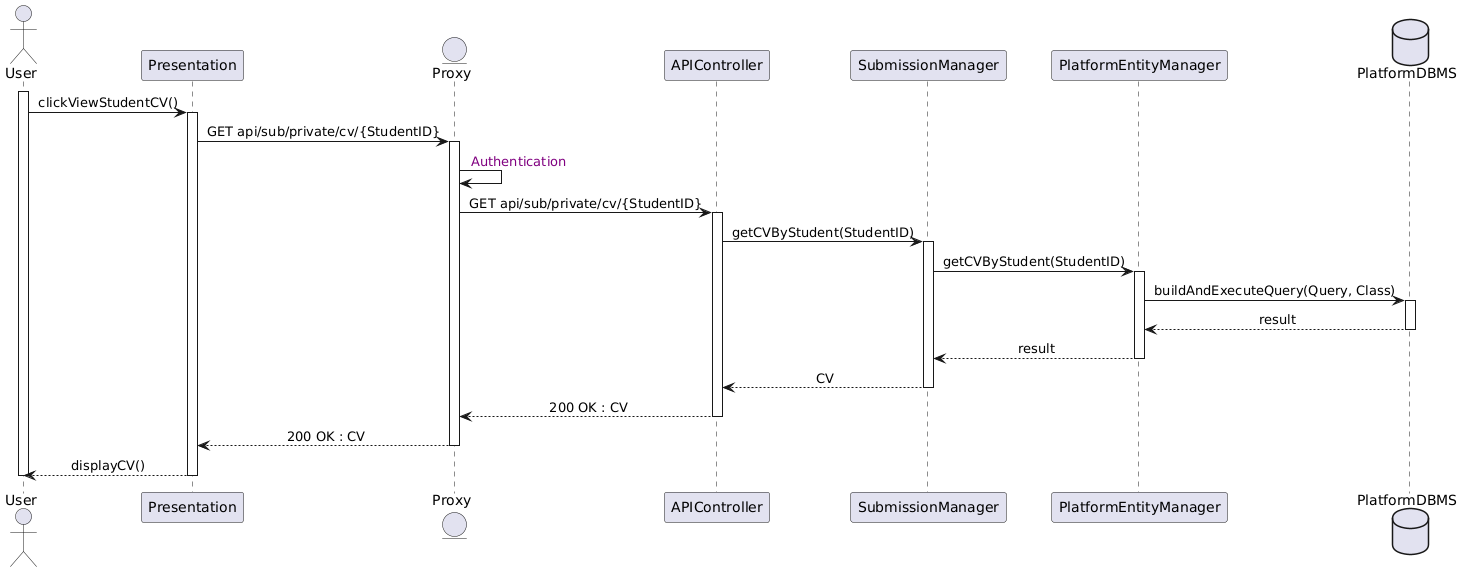
\includegraphics[width=\linewidth]{Latex/Images/DD/SequenceDiagrams/5UserOpensStudentCV.png}
    \caption{User Opens Student CV Sequence Diagram}
    \label{fig:useropensstudentcv}
\end{figure}
By clicking the View Student CV button, the User triggers a GET private request from the Presentation Layer to the Proxy. The Proxy authenticates the request using the Authenticator and forwards it to the APIController in the Application Service.\\
The APIController invokes the SubmissionManager to retrieve the CV of the specified StudentID. The SubmissionManager queries the database through the PlatformEntityManager, which executes the query in the PlatformDBMS and returns the result.\\
The SubmissionManager sends the CV back to the APIController, which forwards it to the Proxy. The Proxy then returns the CV to the Presentation Layer, which displays it to the User.

\subsubsection*{Participant Accepts Match}
\begin{figure}[H]
    \centering
    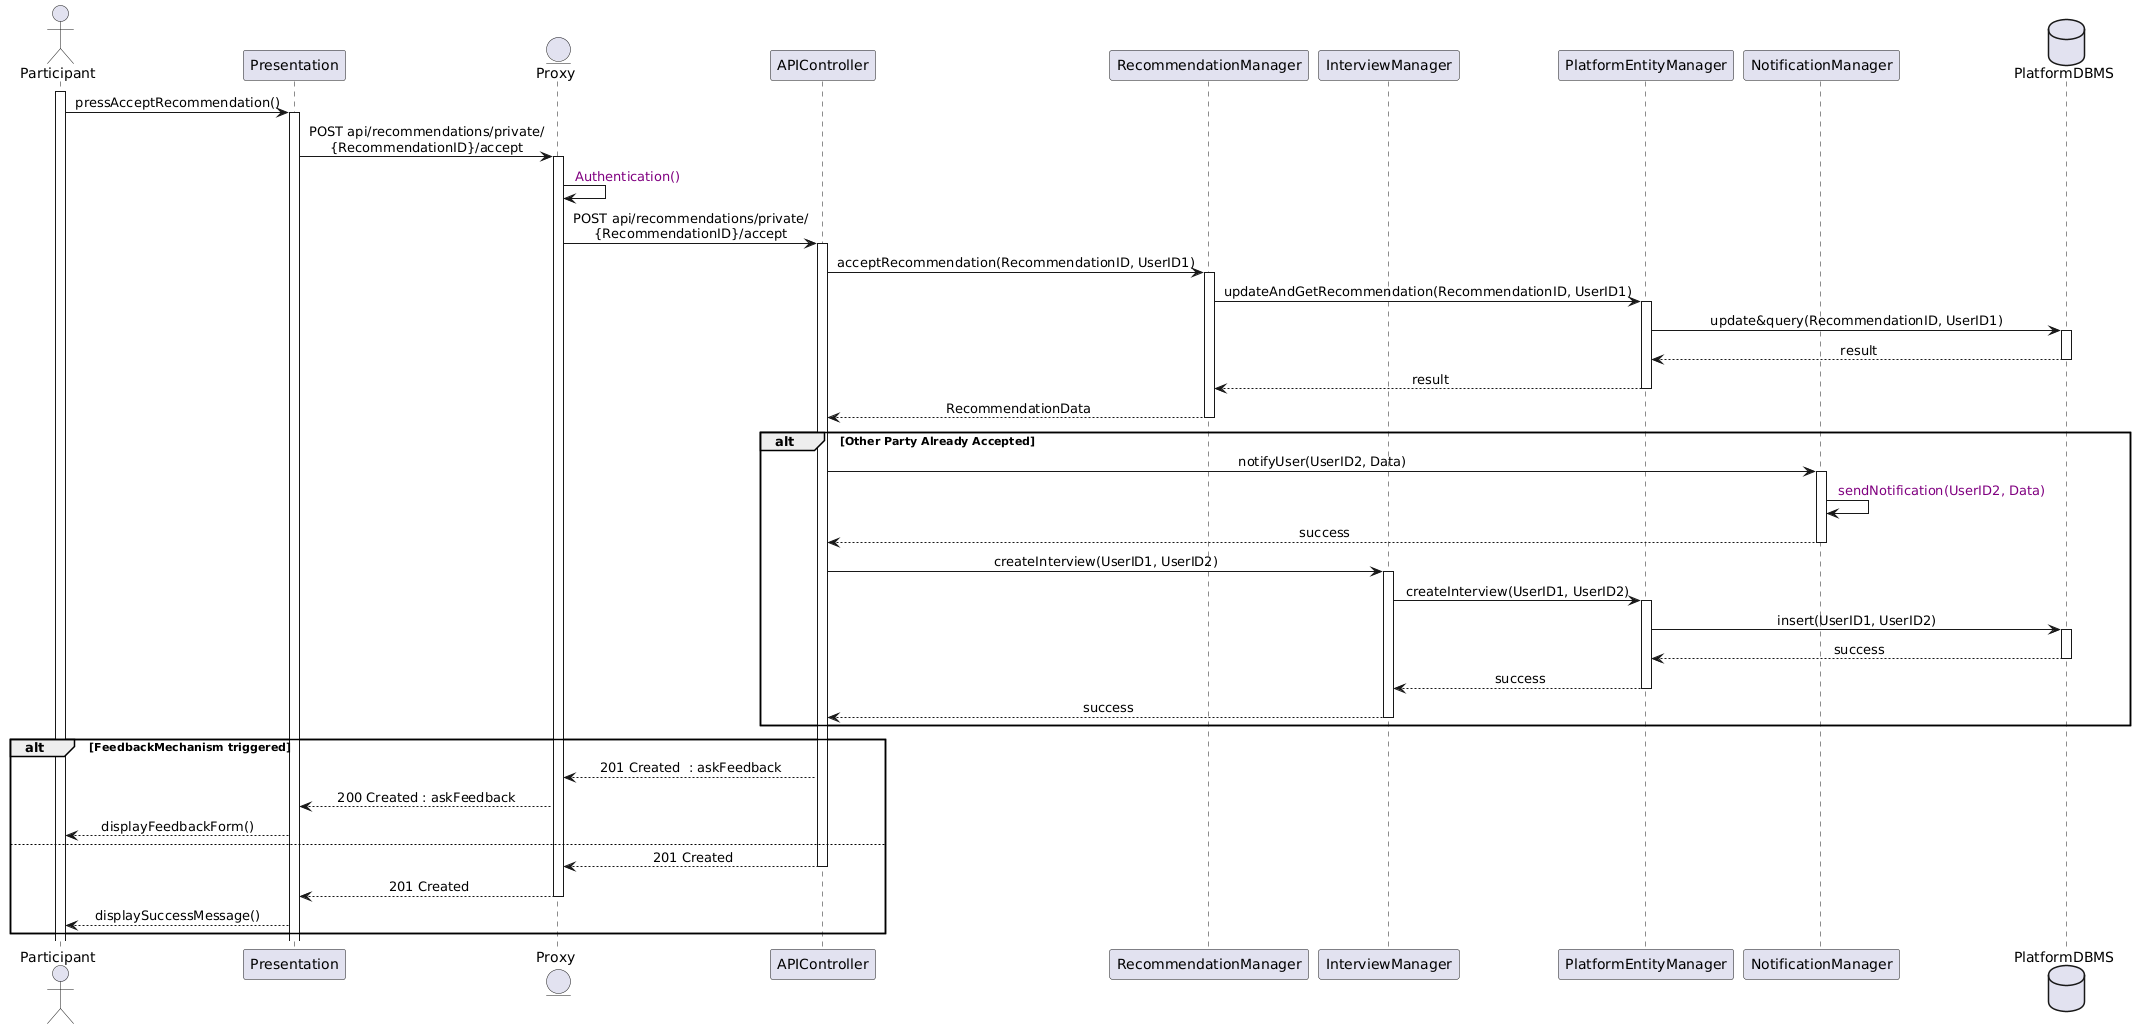
\includegraphics[width=\linewidth]{Latex/Images/DD/SequenceDiagrams/6.1ParticipantAcceptsMatch.png}
    \caption{Participant Accepts Match Sequence Diagram}
    \label{fig:partacceptmatch}
\end{figure}
By pressing the Accept Recommendation button, the Participant triggers a POST private request from the Presentation Layer to the Proxy. The Proxy authenticates the request and forwards it to the APIController in the Application Service.\\
The APIController calls the RecommendationManager to process the acceptance of the recommendation. The RecommendationManager updates and retrieves the recommendation data by interacting with the PlatformEntityManager, which queries the PlatformDBMS.\\
If the other party has already accepted the recommendation, the APIController notifies the second user through the NotificationManager and initiates the creation of an interview using the InterviewManager. The InterviewManager inserts the interview data into the PlatformDBMS through the PlatformEntityManager.\\
If the FeedbackMechanism is triggered, the APIController returns a 201 Created response with a prompt for feedback, which the Presentation Layer displays to the Participant as a feedback form. Otherwise, the APIController simply returns a success message, which the Presentation Layer displays to the Participant.

\subsubsection*{Participant Submits Feedback}
\begin{figure}[H]
    \centering
    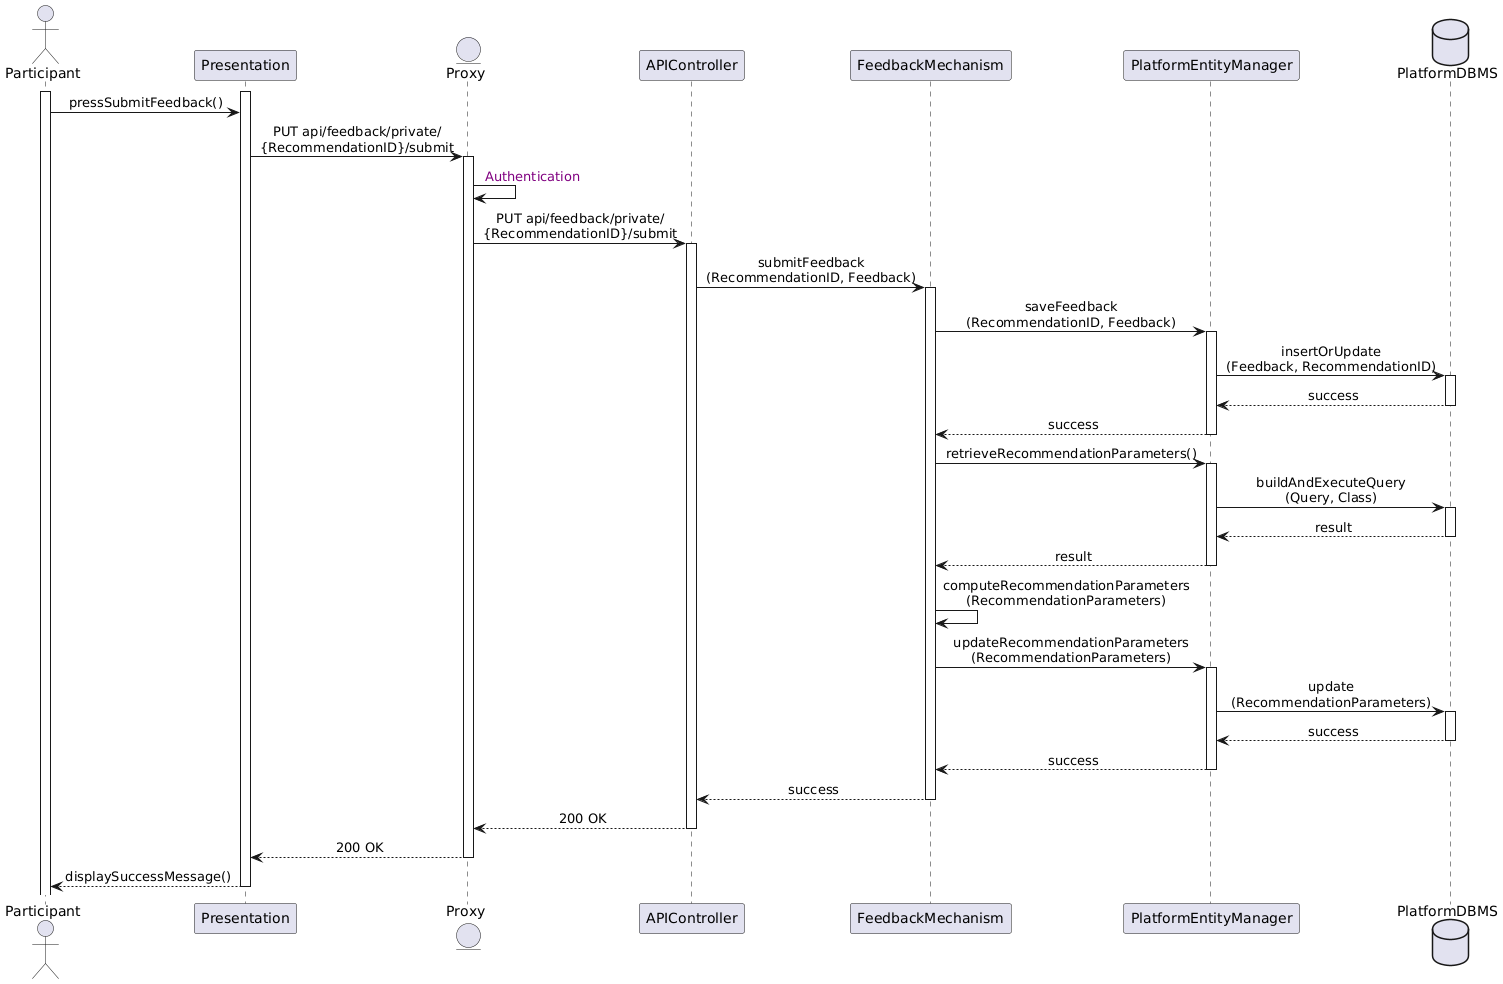
\includegraphics[width=\linewidth]{Latex/Images/DD/SequenceDiagrams/6.2ParticipantSubmitsFeedback.png}
    \caption{Participant Submits Feedback Sequence Diagram}
    \label{fig:partsubfeedback}
\end{figure}
When the Participant presses the Submit Feedback button, the Presentation Layer sends a PUT request with the RecommendationID and feedback data to the Proxy.\\
The Proxy authenticates the request and forwards it to the APIController. The APIController invokes the FeedbackMechanism to handle the feedback submission. The FeedbackMechanism saves the feedback data by interacting with the PlatformEntityManager, which updates the PlatformDBMS.\\
Once the feedback is saved, the FeedbackMechanism retrieves recommendation parameters from the database through the PlatformEntityManager. It computes updated recommendation parameters and saves them back into the database via the PlatformEntityManager.\\
After processing the feedback and updating the recommendation data, the FeedbackMechanism returns a success message to the APIController. The APIController forwards the response to the Proxy, which then sends it to the Presentation Layer. Finally, the Presentation Layer displays a success message to the Participant.
% By pressing the Submit Feedback button, the Participant triggers a PUT private request from the Presentation Layer to the Proxy. The Proxy authenticates the request and forwards it to the APIController in the Application Service.\\
% The APIController invokes the FeedbackMechanism to handle the feedback submission. The FeedbackMechanism saves the feedback data by interacting with the PlatformEntityManager, which updates or inserts the feedback into the PlatformDBMS.\\
% Once the feedback is saved, the FeedbackMechanism retrieves recommendation parameters from the PlatformDBMS through the PlatformEntityManager. It then computes updated recommendation parameters and updates them back in the database via the PlatformEntityManager.\\
% After successfully saving the feedback and updating the recommendation data, the FeedbackMechanism returns a success message to the APIController. The APIController forwards the response to the Proxy, which then sends it to the Presentation Layer. Finally, the Presentation Layer displays a success message to the Participant.

\subsubsection*{Student Sends Spontaneous Application}
\begin{figure}[H]
    \centering
    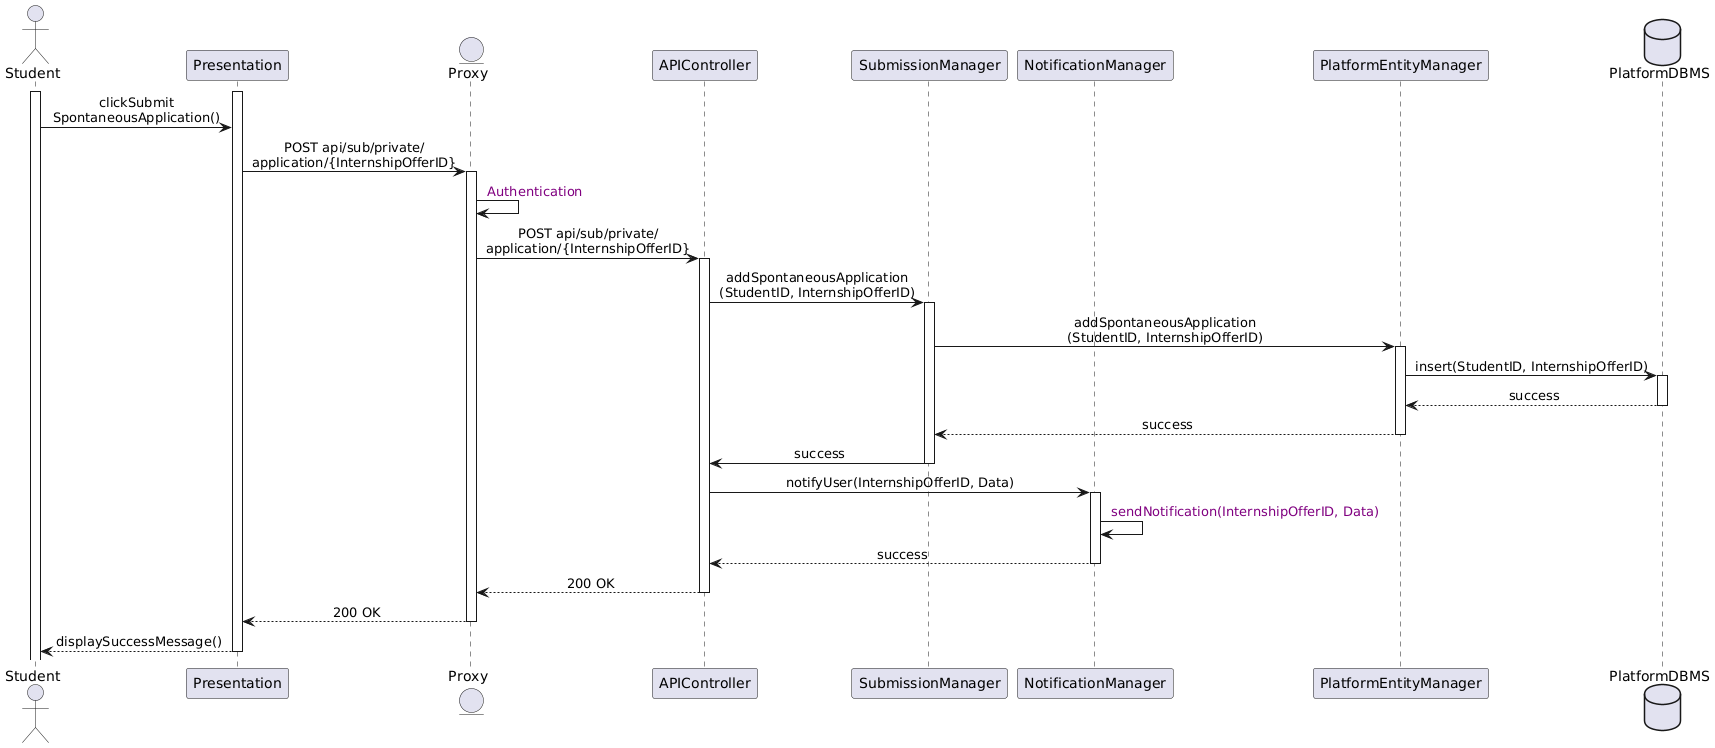
\includegraphics[width=\linewidth]{Latex/Images/DD/SequenceDiagrams/7StudentSendsSpontaneousApplication.png}
    \caption{Student Sends Spontaneous Application Sequence Diagram}
    \label{fig:studsendspontapp}
\end{figure}
By clicking the Submit Spontaneous Application button, the Student triggers a POST private request from the Presentation Layer to the Proxy. The Proxy authenticates the request and forwards it to the APIController in the Application Service.\\
The APIController calls the SubmissionManager to handle the spontaneous application submission. The SubmissionManager insert the users' ID into the database, to represent the application, by interacting with the PlatformEntityManager, which performs the insertion in the PlatformDBMS.\\
Once the application is successfully stored, the APIController invokes the NotificationManager to notify the company about the new application. The NotificationManager sends the notification to the specified company and confirms the success of the operation.\\
Finally, the APIController returns a 200 OK response to the Proxy, which forwards it to the Presentation Layer. The Presentation Layer displays a success message to the Student.

\subsubsection*{Participant Submits Feedback}
\begin{figure}[H]
    \centering
    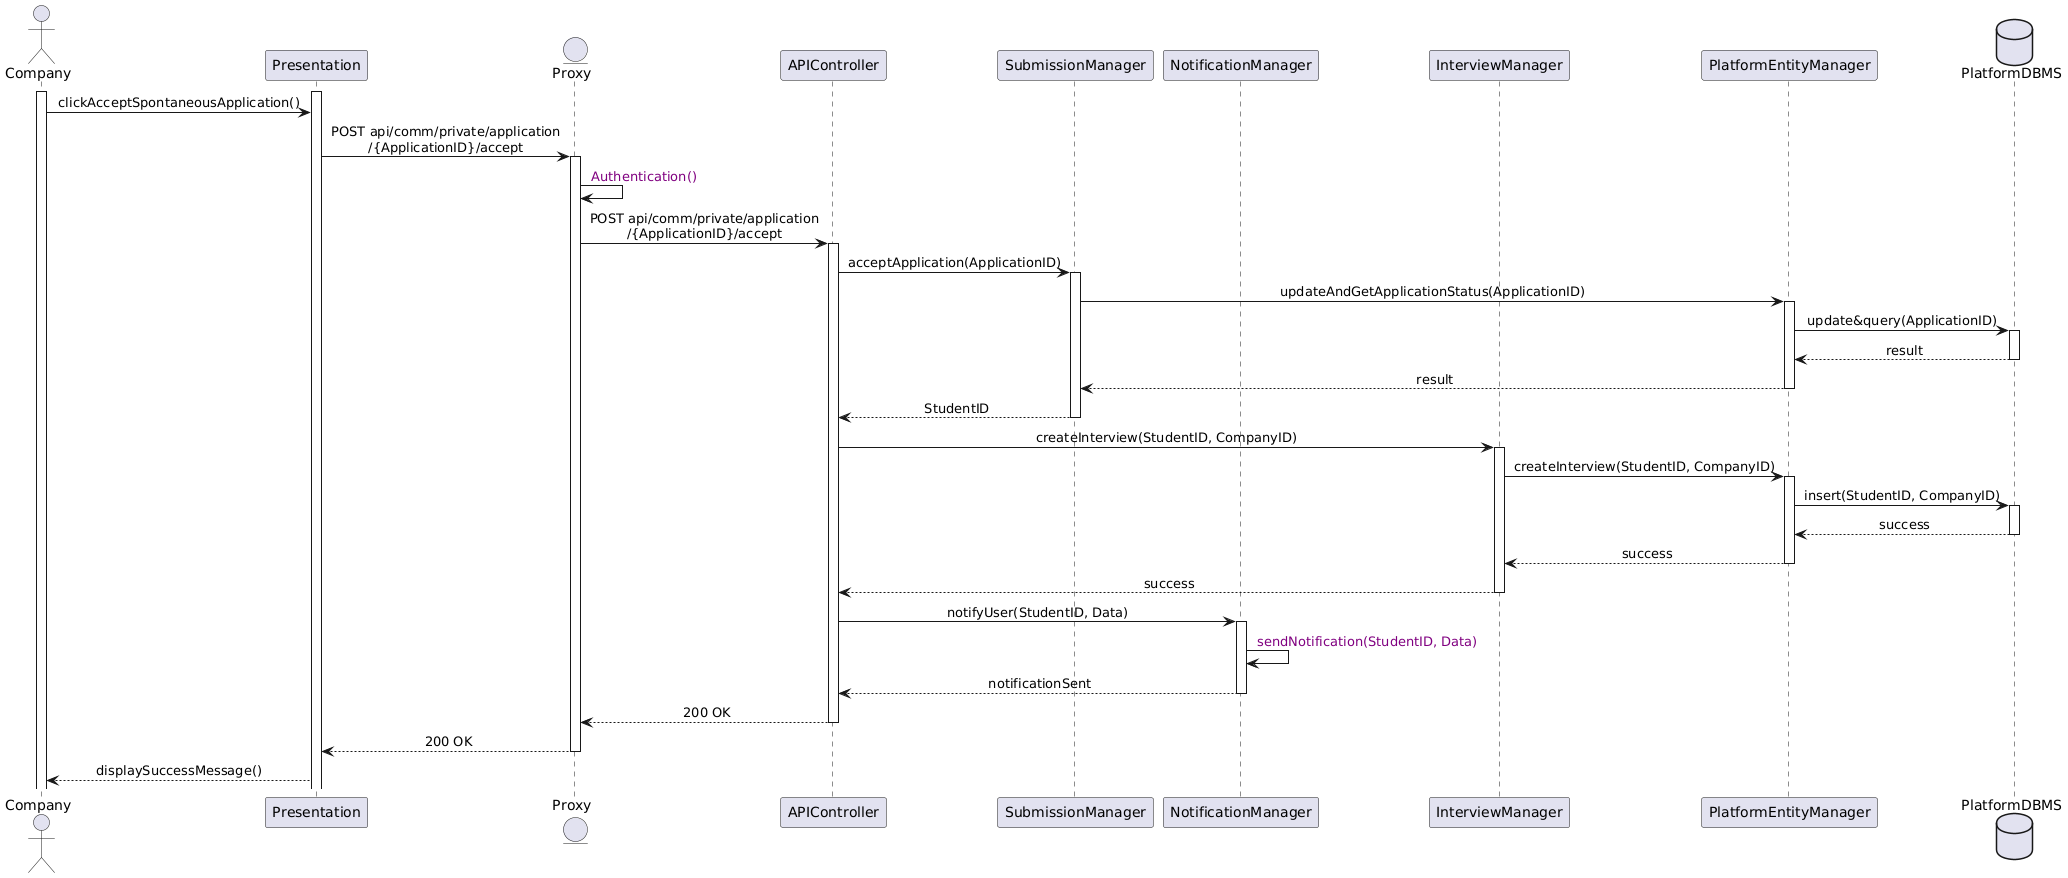
\includegraphics[width=\linewidth]{Latex/Images/DD/SequenceDiagrams/8CompanyAcceptsSpontaneousApplication.png}
    \caption{Company Accept a Spontaneous Application Sequence Diagram}
    \label{fig:compaccspontapp}
\end{figure}
By clicking the Accept Spontaneous Application button, the Company triggers a POST private request from the Presentation Layer to the Proxy. The Proxy authenticates the request and forwards it to the APIController in the Application Service.\\
The APIController calls the SubmissionManager to process the acceptance of the spontaneous application. The SubmissionManager updates the application status and retrieves the StudentID by interacting with the PlatformEntityManager, which queries and updates the PlatformDBMS.\\
With the StudentID retrieved, the APIController invokes the InterviewManager to create an interview for the student and company. The InterviewManager inserts the interview data into the PlatformDBMS through the PlatformEntityManager.\\
Once the interview is successfully created, the APIController calls the NotificationManager to notify the student about the acceptance of their application. The NotificationManager sends the notification and confirms the success of the operation.\\
Finally, the APIController returns a 200 OK response to the Proxy, which forwards it to the Presentation Layer. The Presentation Layer displays a success message to the Company.

\subsubsection*{Student Answers Interview}
\begin{figure}[H]
    \centering
    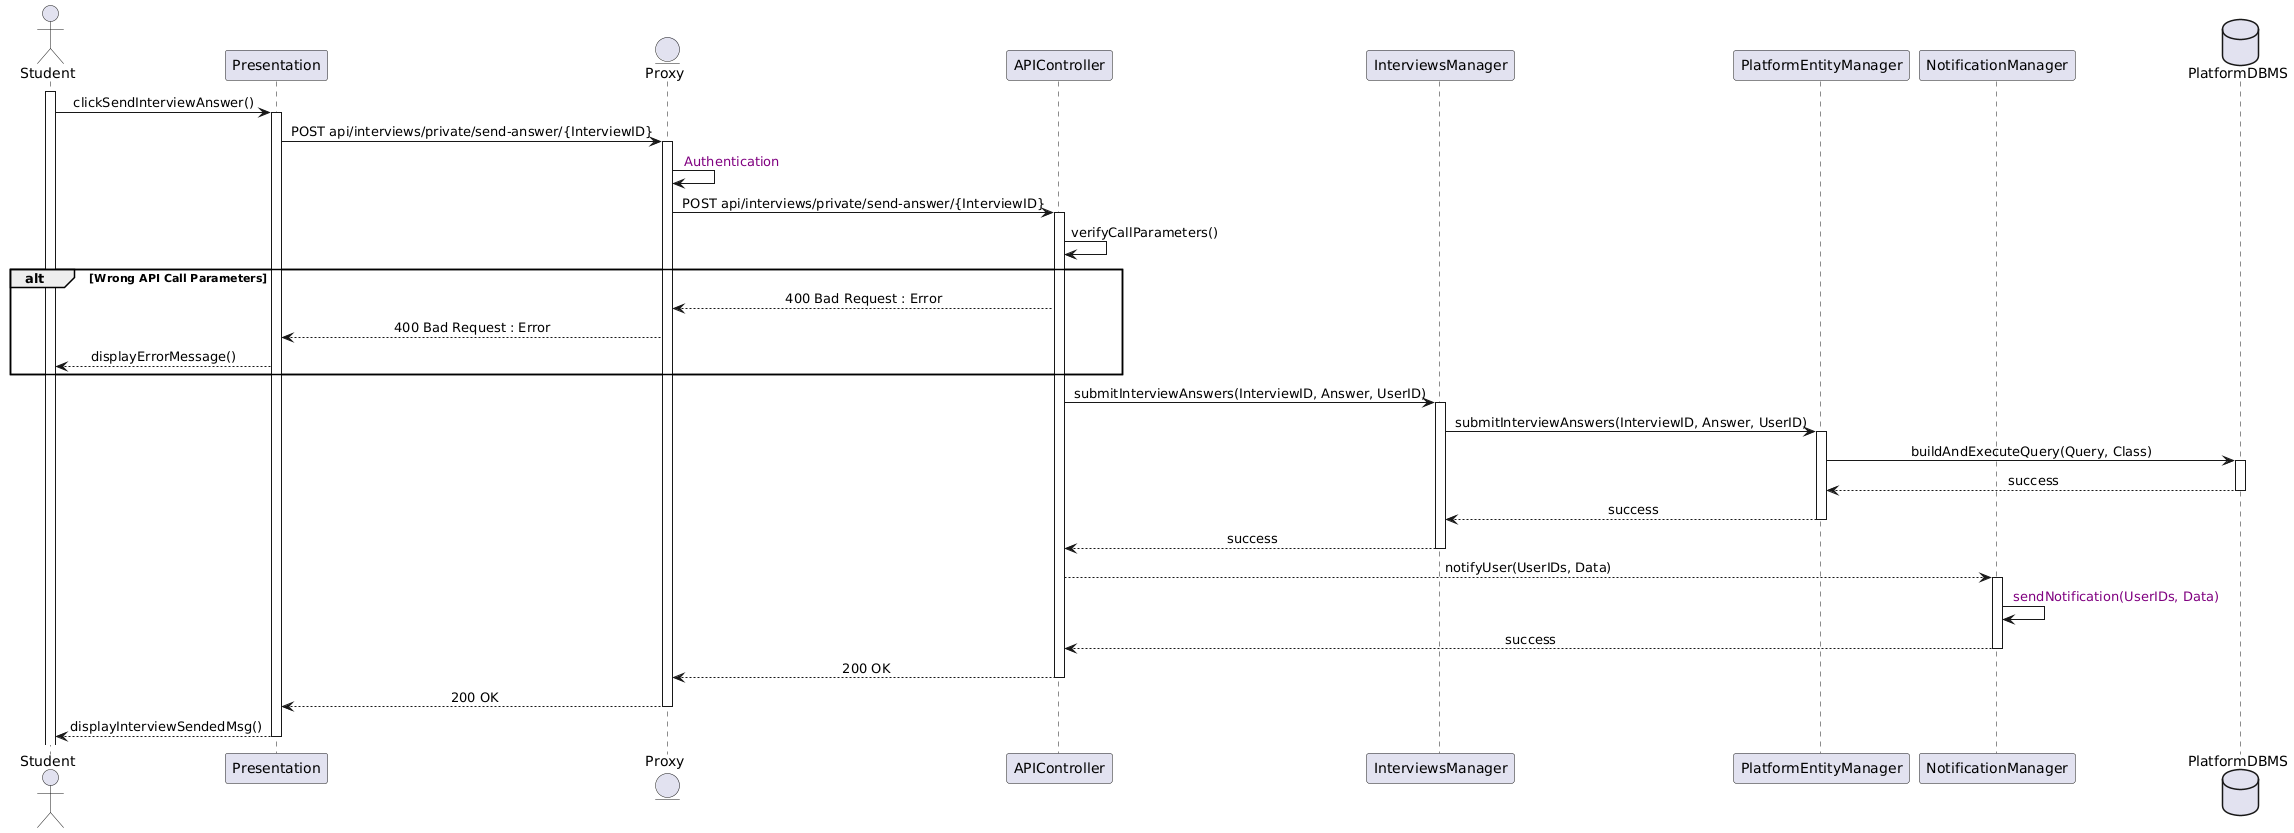
\includegraphics[width=\linewidth]{Latex/Images/DD/SequenceDiagrams/9StudentSubmitInterview.png}
    \caption{Student Answers Interview Sequence Diagram}
    \label{fig:studsubint}
\end{figure}
By clicking the Send Interview Answer button, the Student triggers a POST private request from the Presentation Layer to the Proxy. The Proxy authenticates the request and forwards it to the APIController in the Application Service.\\
The APIController verifies the API call parameters. If the parameters are invalid, it returns a 400 Bad Request error to the Proxy, which forwards it to the Presentation Layer. The Presentation Layer then displays an error message to the Student.\\
If the parameters are valid, the APIController calls the InterviewsManager to save the interview answers. The InterviewsManager updates the database by interacting with the PlatformEntityManager, which executes the required query in the PlatformDBMS.\\
After the interview answers are successfully stored, the APIController invokes the NotificationManager to notify relevant users about the submission. The NotificationManager sends the notification and confirms its success.\\
Finally, the APIController returns a 200 OK response to the Proxy, which forwards it to the Presentation Layer. The Presentation Layer displays a success message to the Student, indicating that the interview answers have been submitted.

\subsubsection*{Company Submits Interview}
\begin{figure}[H]
    \centering
    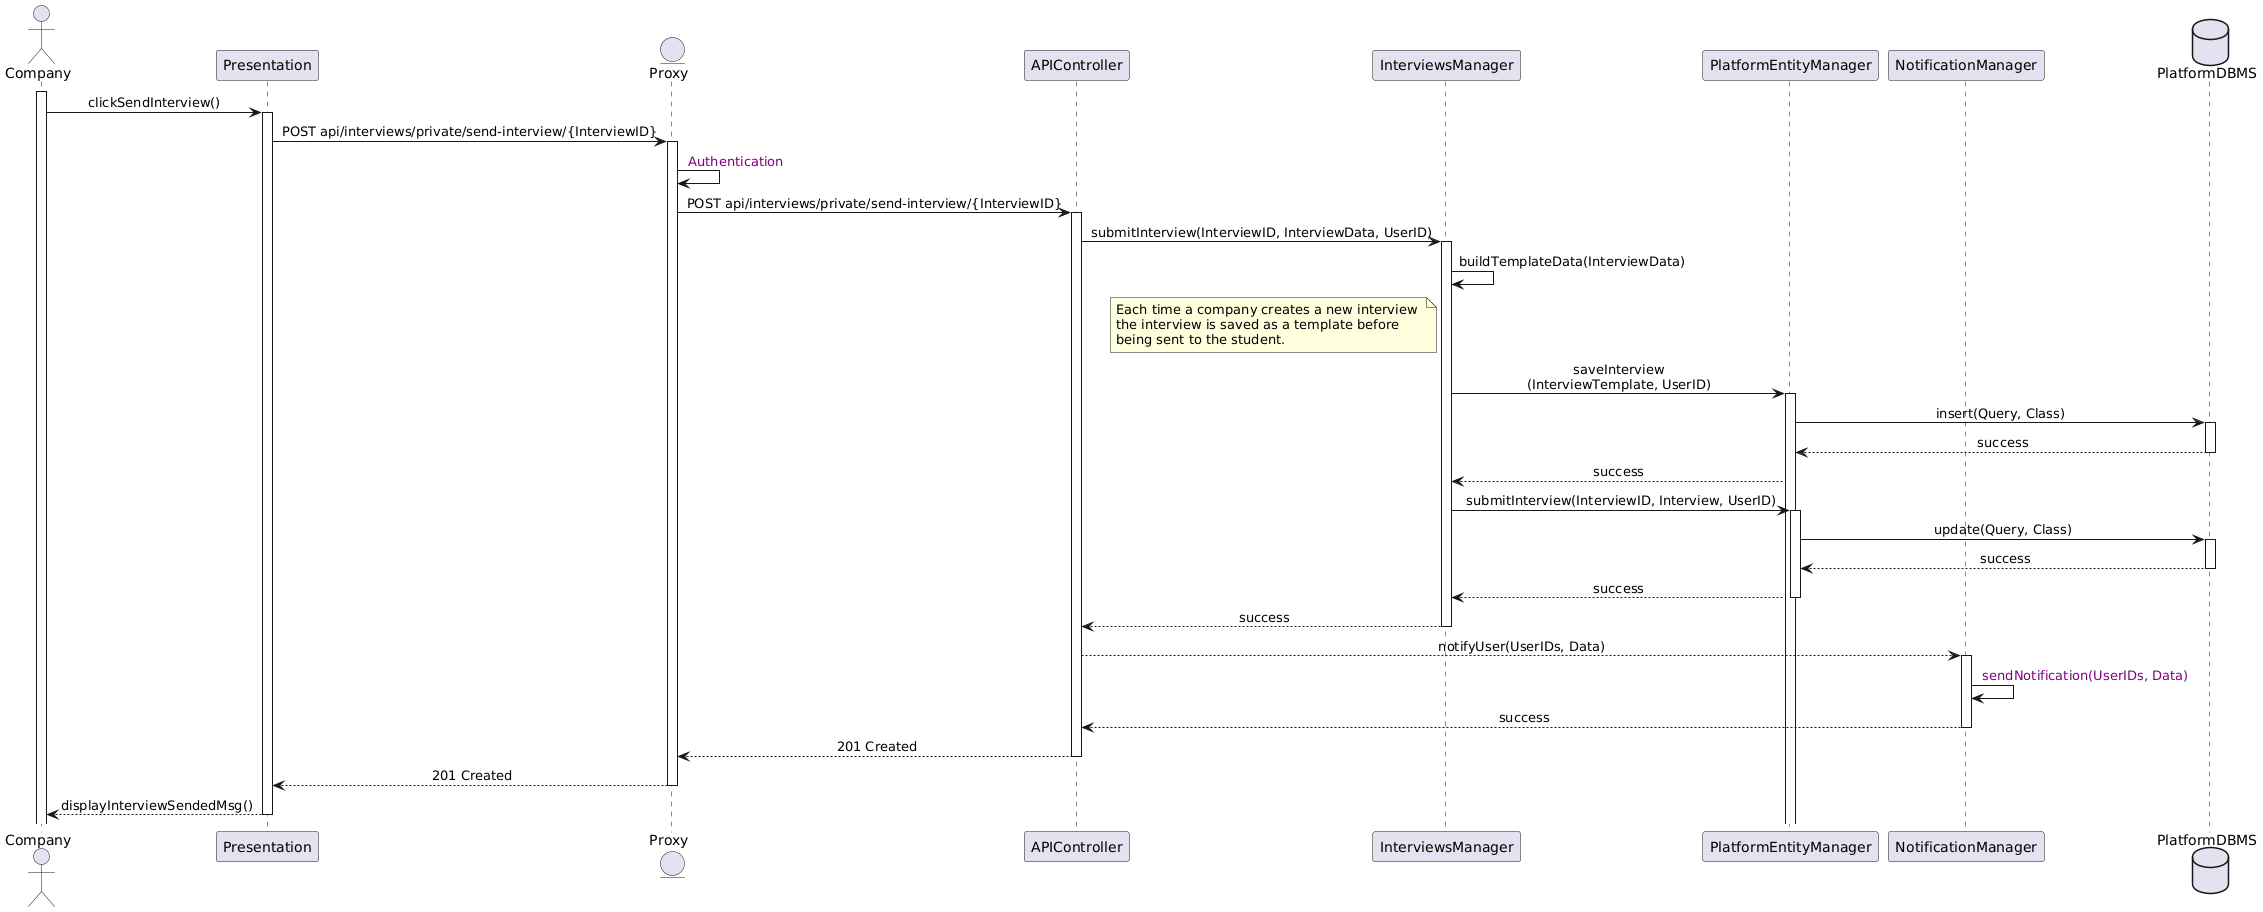
\includegraphics[width=\linewidth]{Latex/Images/DD/SequenceDiagrams/10CompanySubmitInterview.png}
    \caption{Company Submits Interview Sequence Diagram}
    \label{fig:compsubint}
\end{figure}
By clicking the Send Interview button, the Company triggers a POST private request from the Presentation Layer to the Proxy. The Proxy authenticates the request and forwards it to the APIController in the Application Service.\\
The APIController invokes the InterviewsManager to handle the interview submission. The InterviewsManager first builds the interview template data from the provided InterviewData. Each time a company creates a new interview, it is saved as a template before being sent to the student.\\
The InterviewsManager saves the interview template to the database via the PlatformEntityManager, which performs the insertion in the PlatformDBMS. After successfully saving the template, the InterviewsManager submits the interview by updating the relevant data in the PlatformDBMS through the PlatformEntityManager.\\
Once the interview is successfully stored, the APIController calls the NotificationManager to notify the student about the new interview. The NotificationManager sends the notification and confirms its success.\\
Finally, the APIController returns a 201 Created response to the Proxy, which forwards it to the Presentation Layer. The Presentation Layer displays a success message to the Company, indicating that the interview has been sent.

\subsubsection*{Company Creates Template Interview}
\begin{figure}[H]
    \centering
    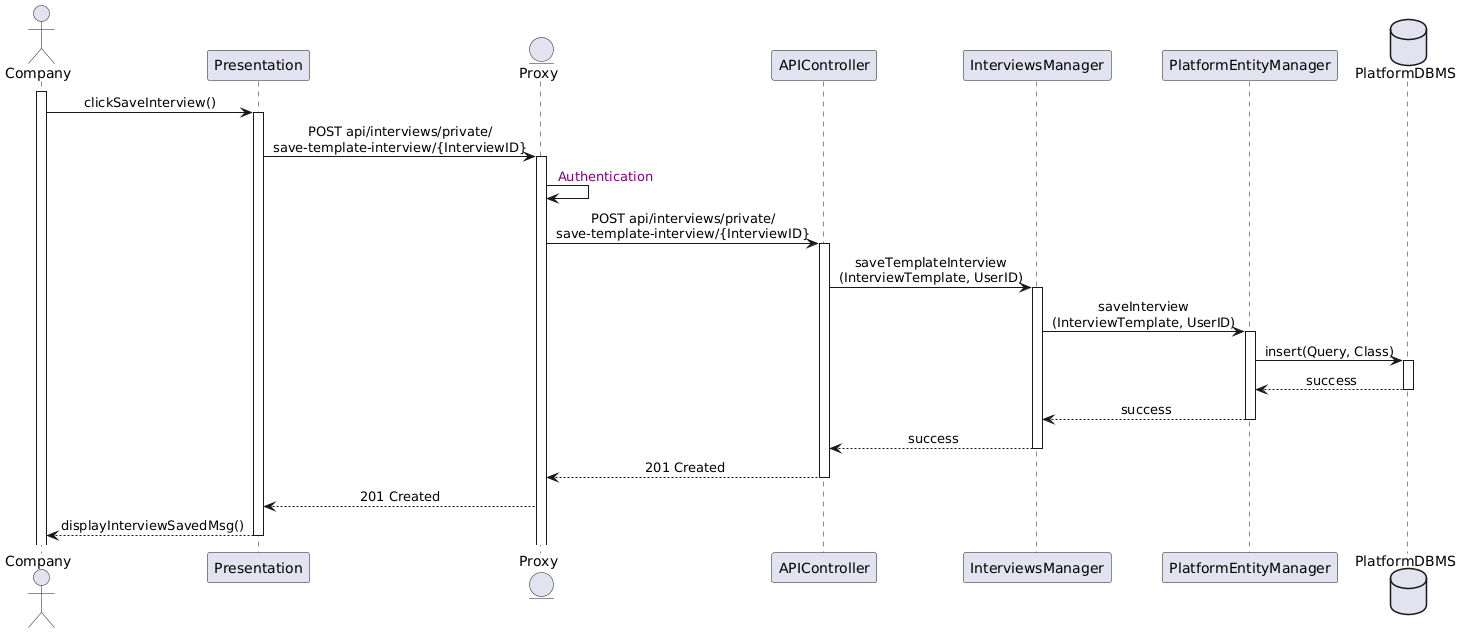
\includegraphics[width=\linewidth]{Latex/Images/DD/SequenceDiagrams/11CompanyCreateTemplateInterview.png}
    \caption{Company Creates Template Interview Sequence Diagram}
    \label{fig:compcretempint}
\end{figure}
By clicking the Save Interview button, the Company triggers a POST private request from the Presentation Layer to the Proxy. The Proxy authenticates the request and forwards it to the APIController in the Application Service.\\
The APIController invokes the InterviewsManager to handle the saving of the interview template. The InterviewsManager saves the provided InterviewTemplate to the database via the PlatformEntityManager. The PlatformEntityManager inserts the template data into the PlatformDBMS.\\
Once the interview template is successfully stored, the APIController returns a 201 Created response to the Proxy, which forwards it to the Presentation Layer. The Presentation Layer displays a success message to the Company, indicating that the interview template has been saved.

\subsubsection*{Company Evaluates Interview}
\begin{figure}[H]
    \centering
    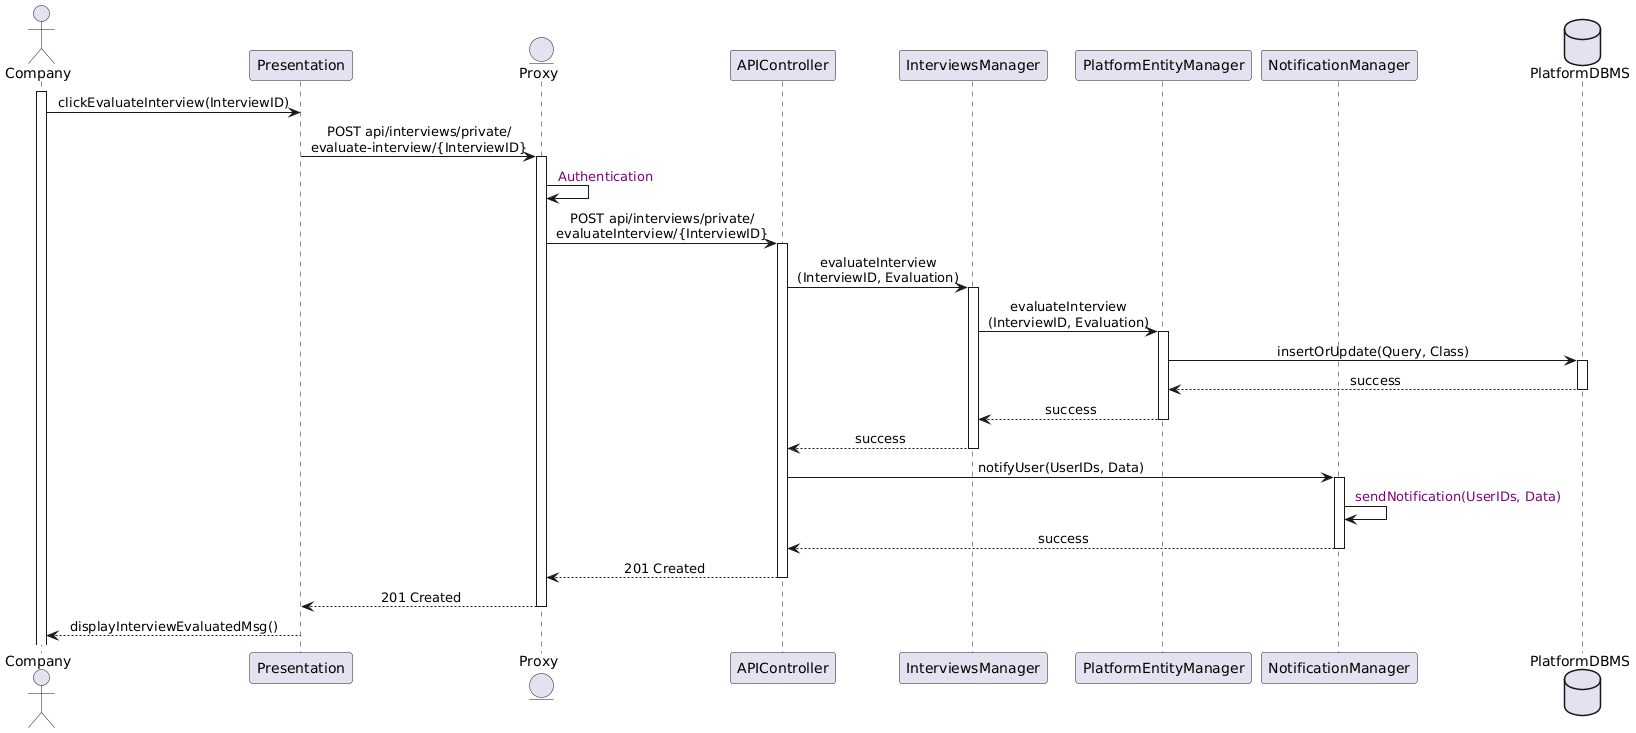
\includegraphics[width=\linewidth]{Latex/Images/DD/SequenceDiagrams/12CompanyEvaluatesInterview.png}
    \caption{Company Evaluates Interview Sequence Diagram}
    \label{fig:compevalint}
\end{figure}
By clicking the Evaluate Interview button, the Company triggers a POST private request from the Presentation Layer to the Proxy. The Proxy authenticates the request and forwards it to the APIController in the Application Service.\\
The APIController calls the InterviewsManager to handle the evaluation of the interview. The InterviewsManager processes the evaluation and updates the database through the PlatformEntityManager. The PlatformEntityManager performs an insert or update operation in the PlatformDBMS with the evaluation data.\\
After successfully saving the evaluation, the APIController triggers a notification to the student through the NotificationManager. The NotificationManager sends the notification and confirms its success.\\
The APIController returns a 201 Created response to the Proxy, which forwards it to the Presentation Layer. The Presentation Layer displays a success message to the Company, confirming that the interview has been evaluated.\\
If the Company needs to evaluate individual questions within the interview, they can access the interview through the dashboard. By navigating to the Dashboard Interviews page, the Company sends a GET request to retrieve a list of interviews. Once the interviews are displayed, the Company can click on a specific interview to access the detailed evaluation page.

\subsubsection*{Student Sees Spontaneous Application}
\begin{figure}[H]
    \centering
    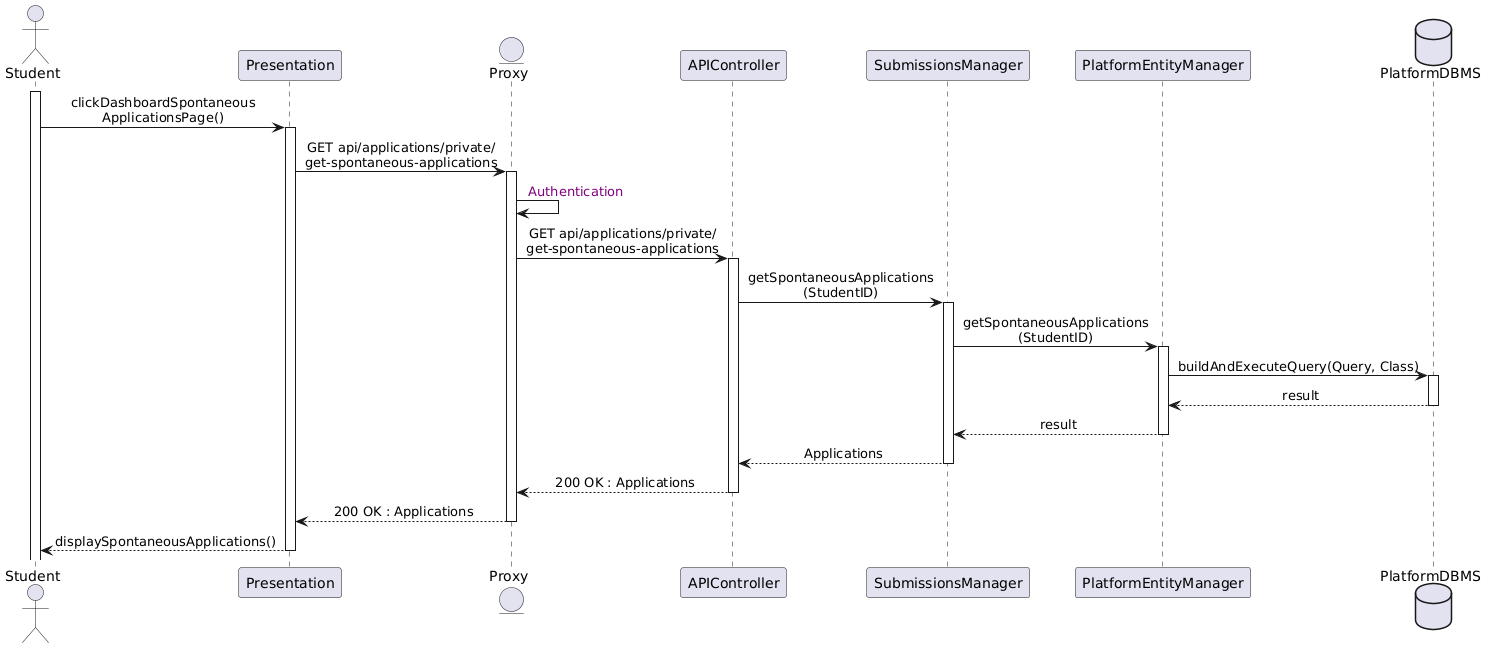
\includegraphics[width=\linewidth]{Latex/Images/DD/SequenceDiagrams/13StudentSeeSpontaneousApplications.png}
    \caption{Student Sees Spontaneous Application Sequence Diagram}
    \label{fig:studseespontapp}
\end{figure}
By clicking the Dashboard Spontaneous Applications page, the Student triggers a GET private request from the Presentation Layer to the Proxy. The Proxy authenticates the request and forwards it to the APIController in the Application Service.\\
The APIController calls the SubmissionsManager to retrieve the list of spontaneous applications related to the Student. The SubmissionsManager queries the database through the PlatformEntityManager. The PlatformEntityManager executes the query in the PlatformDBMS and retrieves the results.\\
The results are returned step-by-step: from the PlatformEntityManager to the SubmissionsManager, from the SubmissionsManager to the APIController, and finally to the Proxy. The Proxy sends a 200 OK response with the list of applications back to the Presentation Layer.\\
The Presentation Layer displays the retrieved spontaneous applications to the Student, allowing them to review their submissions.

\subsubsection*{Participant Sees Matches}
\begin{figure}[H]
    \centering
    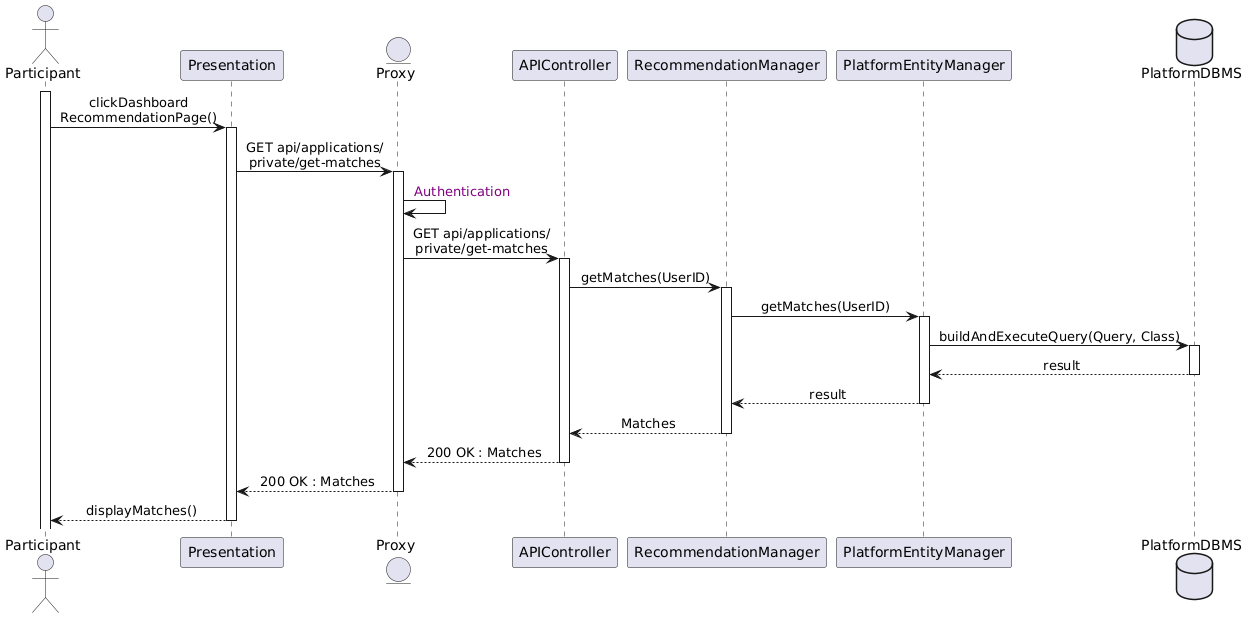
\includegraphics[width=\linewidth]{Latex/Images/DD/SequenceDiagrams/14ParticipantSeesMatches.png}
    \caption{Participant Sees Matches Sequence Diagram}
    \label{fig:partseesmatches}
\end{figure}
By clicking the Dashboard Recommendation page, the Participant triggers a GET private request from the Presentation Layer to the Proxy. The Proxy authenticates the request and forwards it to the APIController in the Application Service.\\
The APIController calls the RecommendationManager to retrieve matches associated with the Participant's UserID. The RecommendationManager queries the database through the PlatformEntityManager. The PlatformEntityManager executes the query in the PlatformDBMS and retrieves the results.\\
The results are returned step-by-step: from the PlatformEntityManager to the RecommendationManager, from the RecommendationManager to the APIController, and finally to the Proxy. The Proxy sends a 200 OK response with the list of matches back to the Presentation Layer.\\
The Presentation Layer displays the retrieved matches to the Participant, allowing them to review their recommendations.

\subsubsection*{User Responds To Communication}
\begin{figure}[H]
    \centering
    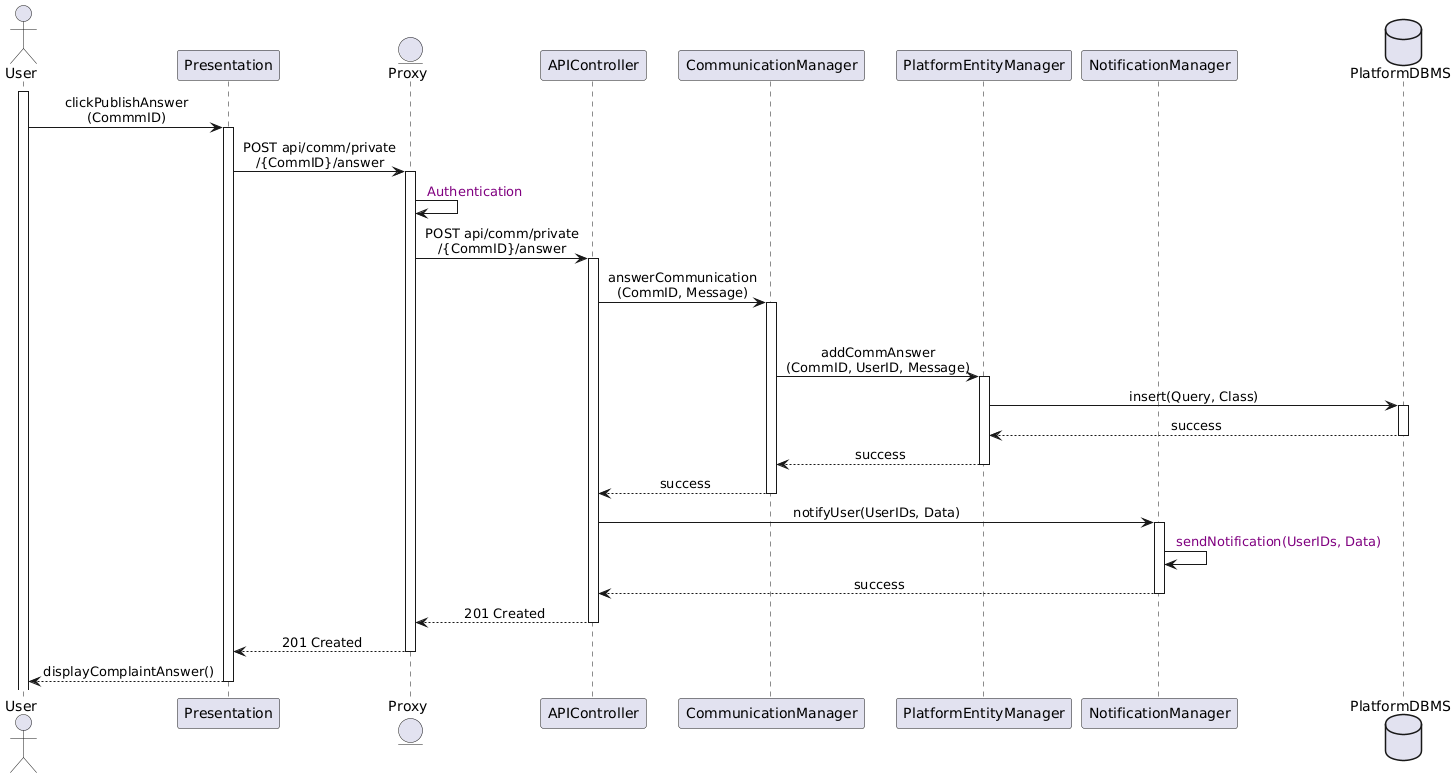
\includegraphics[width=\linewidth]{Latex/Images/DD/SequenceDiagrams/15UserRespondsToComm.png}
    \caption{User Responds To Communication Sequence Diagram}
    \label{fig: usrespondcomm}
\end{figure}
By clicking the Publish Answer button, the User initiates a POST private API call from the Presentation Layer to the Proxy. The request contains the CommID, the User's message, and their authentication token.\\
The Proxy first validates the token using its authentication middleware and forwards the request to the APIController. The APIController processes the request by calling the CommunicationManager to handle the submission.\\
The CommunicationManager interacts with the PlatformEntityManager, which constructs a query to insert the answer (identified by CommID and associated with the UserID) into the database (PlatformDBMS). Upon successful insertion, a confirmation is passed back through the PlatformEntityManager and CommunicationManager to the APIController.\\
Subsequently, the APIController invokes the NotificationManager to notify relevant users about the new message. The NotificationManager sends notifications and confirms the operation's success.\\
Finally, the APIController returns a 201 Created response to the Proxy, which forwards it to the Presentation Layer. The Presentation Layer displays a success message to the User, confirming the answer has been published successfully.

\subsubsection*{User Opens a Complaint}
\begin{figure}[H]
    \centering
    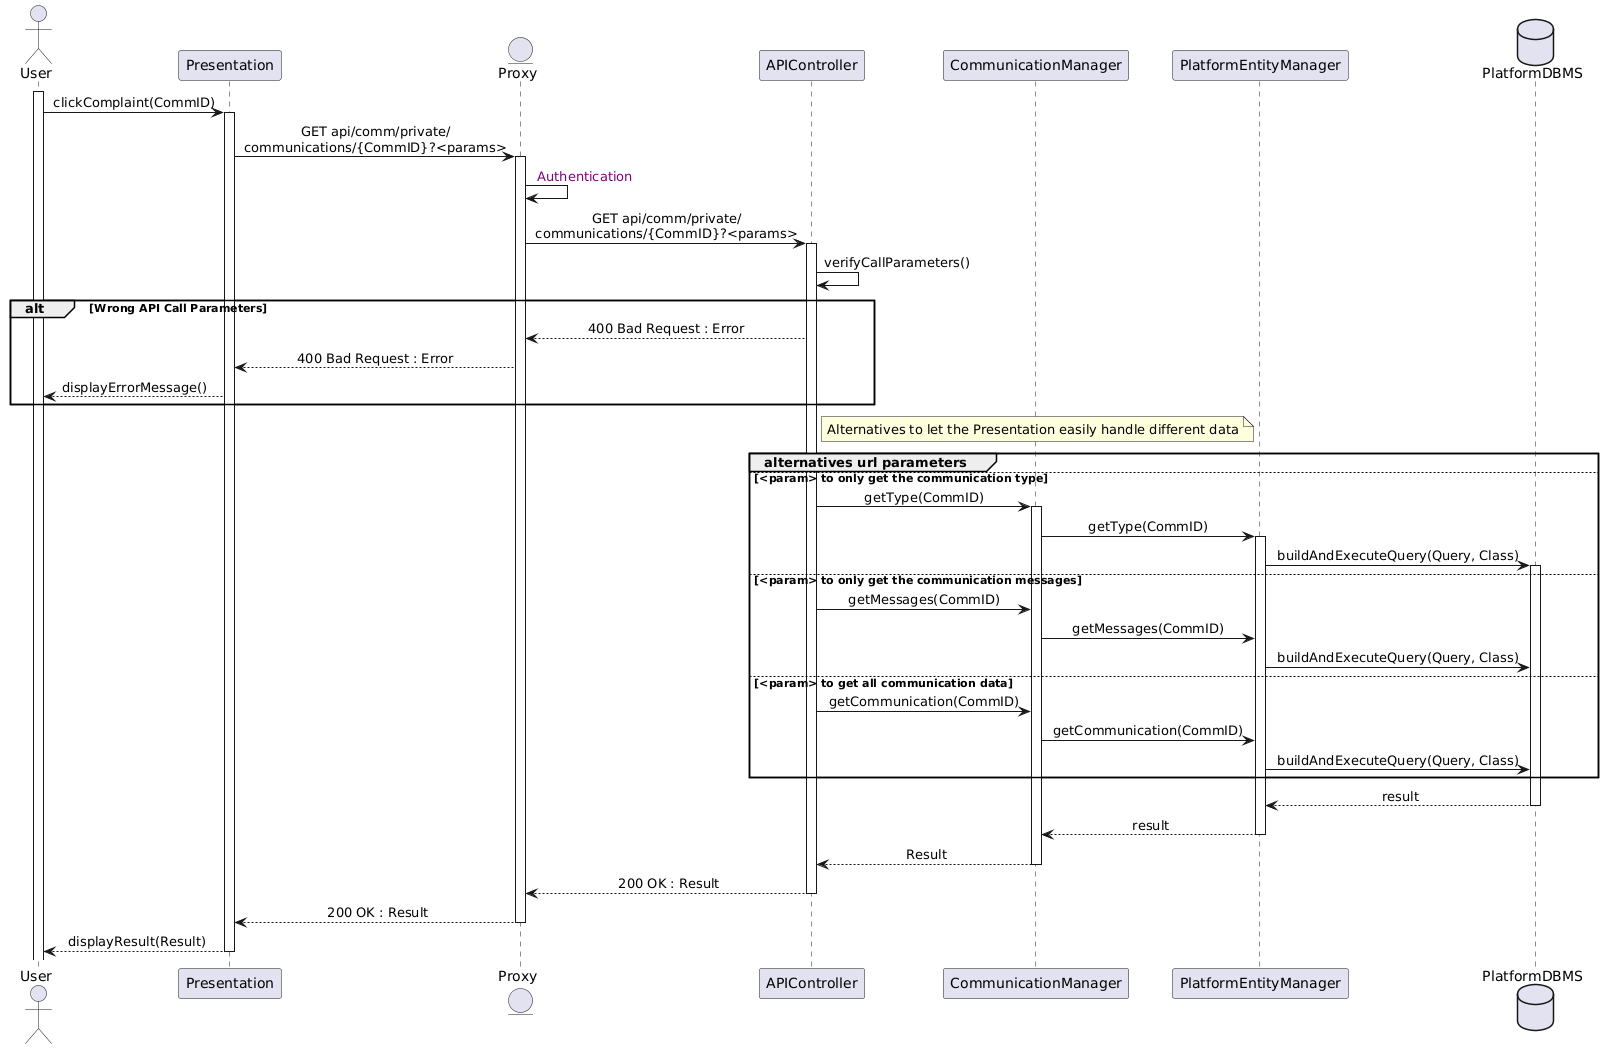
\includegraphics[width=\linewidth]{Latex/Images/DD/SequenceDiagrams/16UserOpensComplaint.png}
    \caption{User Opens Complaint Sequence Diagram}
    \label{fig:usopencomp}
\end{figure}
When the User clicks on a complaint, a GET private API call is sent from the Presentation Layer to the Proxy. The request includes the CommID and optional URL parameters that specify the type of data to retrieve.
\\
The Proxy validates the User's authentication token and forwards the request to the APIController. The APIController verifies the call parameters to ensure they are correct. If any parameter is invalid, the APIController responds with a 400 Bad Request error, which is forwarded by the Proxy to the Presentation Layer. The Presentation Layer displays an error message to the User.\\
If the parameters are valid, the APIController processes the request based on the specified URL parameter:
\begin{itemize}
\item If the parameter requests only the communication type, the APIController calls the CommunicationManager to retrieve the type of communication associated with the CommID.
\item If the parameter requests only the communication messages, the APIController retrieves the messages through the CommunicationManager.
\item  If the parameter requests all communication data, the APIController retrieves the complete communication details via the CommunicationManager.
\end{itemize}
The CommunicationManager queries the PlatformDBMS through the PlatformEntityManager to fetch the requested data. Once the database query is executed successfully, the result is passed back to the APIController.\\
The APIController returns a 200 OK response containing the requested data to the Proxy. The Proxy forwards this response to the Presentation Layer, which displays the result to the User.
\subsubsection*{Participant Creates a Complaint}
\begin{figure}[H]
    \centering
    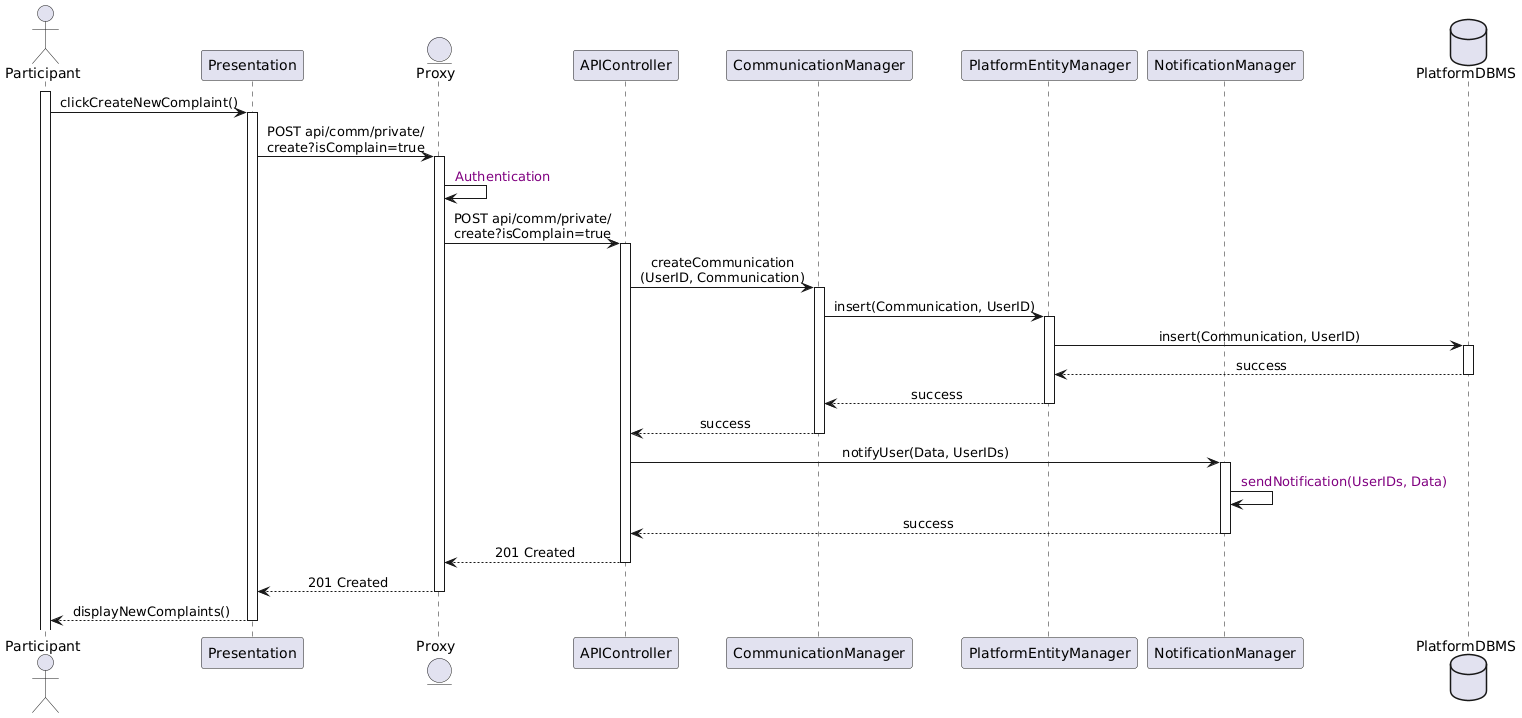
\includegraphics[width=\linewidth]{Latex/Images/DD/SequenceDiagrams/17ParticipantCreatesAComplaint.png}
    \caption{Participant Creates a Complaint Sequence Diagram}
    \label{fig:partcratacomp}
\end{figure}
When the Participant initiates the creation of a new complaint by clicking the corresponding button, the Presentation Layer sends a POST request to the Proxy. The Proxy authenticates the request and forwards it to the APIController.\\
The APIController invokes the CommunicationManager to handle the creation of the new complaint. The CommunicationManager interacts with the PlatformEntityManager to insert the complaint data into the database. The PlatformEntityManager performs this operation by communicating with the PlatformDBMS.\\
Once the complaint is successfully stored in the database, the CommunicationManager returns a success response to the APIController. Subsequently, the APIController triggers the NotificationManager to notify relevant users about the new complaint. After the notifications are sent, a success response propagates back through the Proxy to the Presentation Layer.\\
Finally, the Presentation Layer displays the newly created complaint to the Participant.

\subsubsection*{User Sees his Communications Page}
\begin{figure}[H]
    \centering
    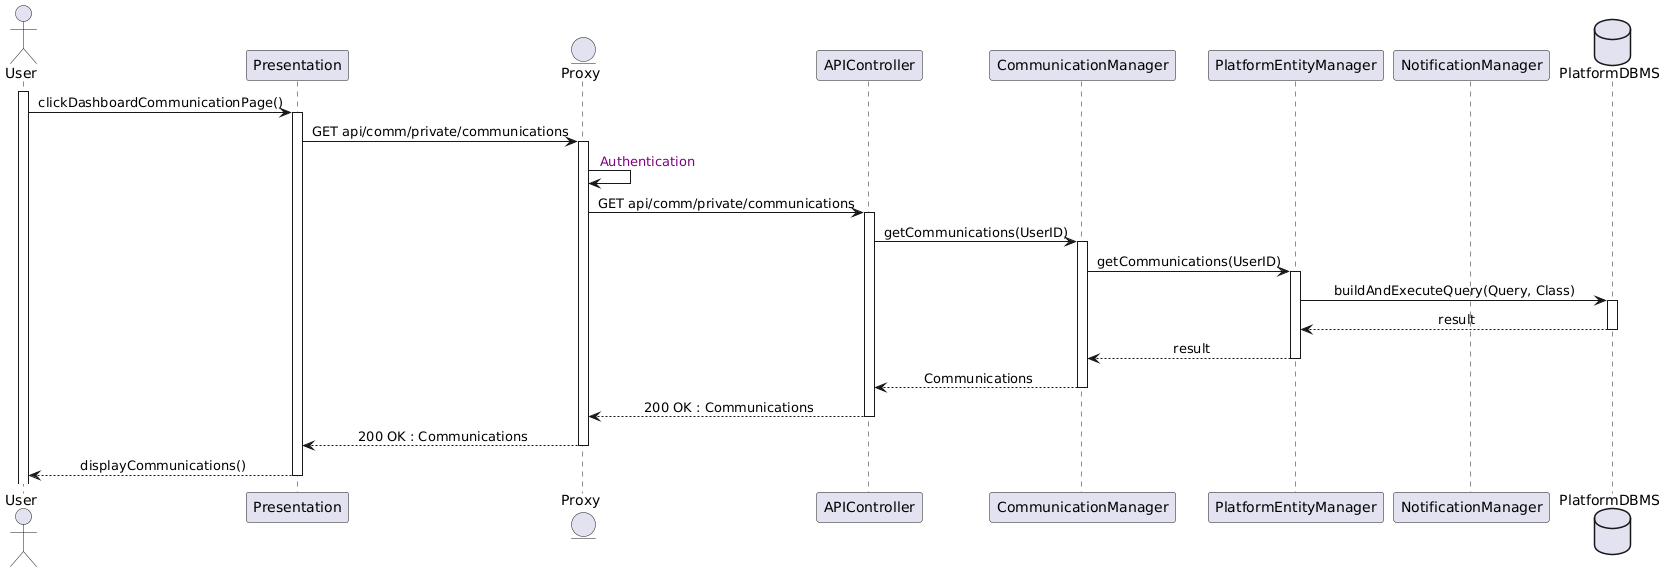
\includegraphics[width=\linewidth]{Latex/Images/DD/SequenceDiagrams/18UserSeesHisCommunicationsPage.png}
    \caption{User Communications Page Sequence Diagram}
    \label{fig:uscommpage}
\end{figure}
When the User clicks the "Dashboard Communication Page" button, the Presentation Layer sends a GET private API call to the Proxy.\\
The Proxy validates the User's authentication token and forwards the request to the APIController. The APIController triggers the CommunicationManager to fetch the list of communications associated with the UserID.\\
The CommunicationManager sends a query to the PlatformEntityManager, which interacts with the PlatformDBMS to retrieve the requested data. Once the database returns the results, the PlatformEntityManager forwards them back to the CommunicationManager.\\
The CommunicationManager passes the fetched communications to the APIController, which returns a 200 OK response to the Proxy, including the list of communications. The Proxy forwards this response to the Presentation Layer.\\
Finally, the Presentation Layer displays the list of communications to the User.
\subsubsection*{University Interrupts an Ongoing Internship}
\begin{figure}[H]
    \centering
    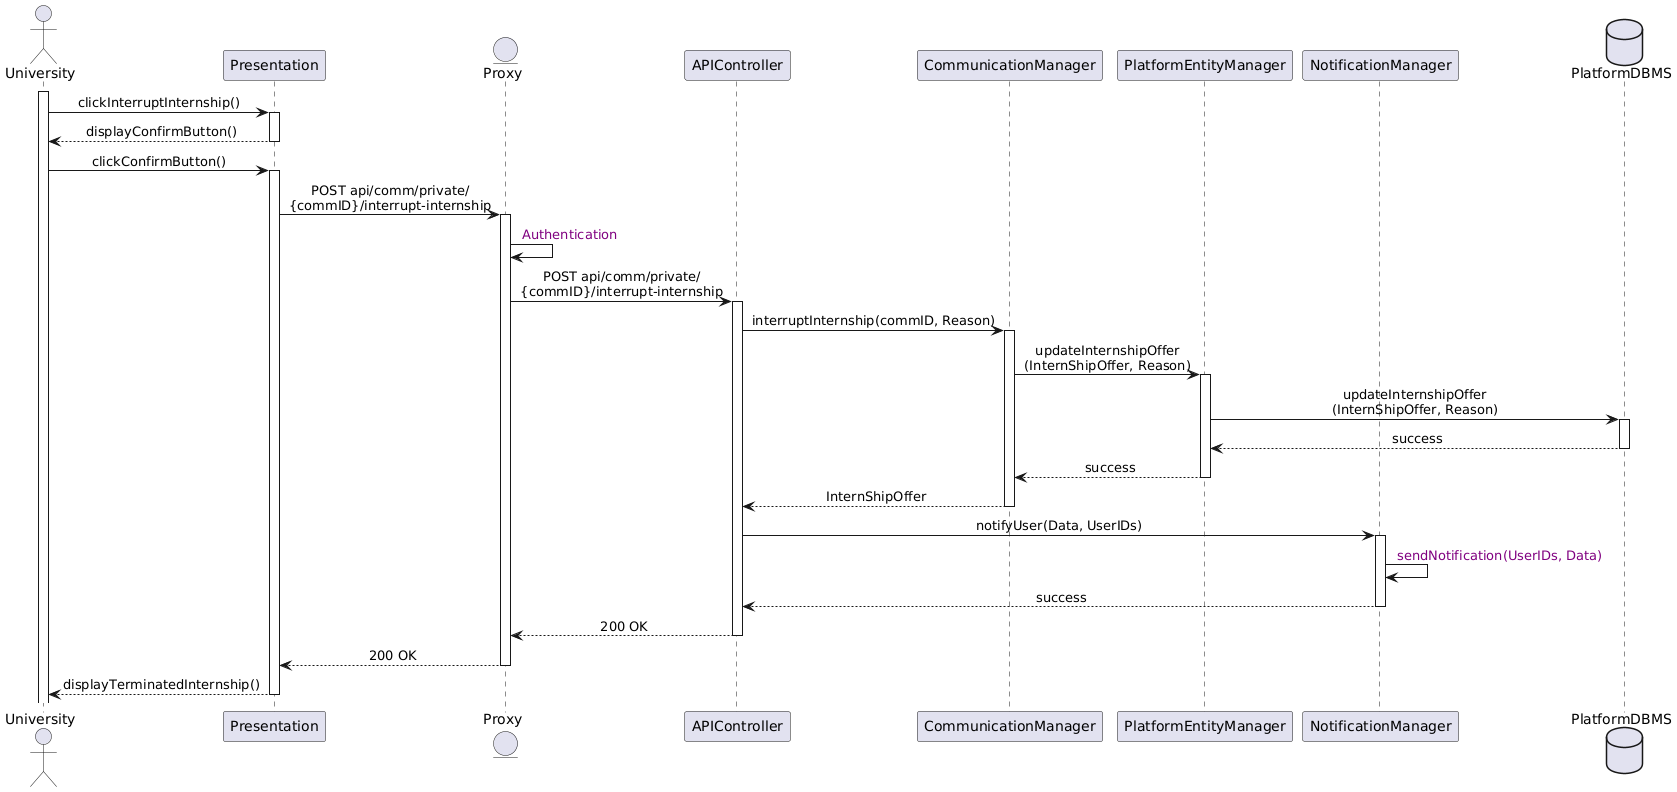
\includegraphics[width=\linewidth]{Latex/Images/DD/SequenceDiagrams/19UniversityInterruptsIntership.png}
    \caption{ University Interrupts Internship Sequence Diagram}
    \label{fig:unintint}
\end{figure}
When the University initiates the process to interrupt an internship by clicking the appropriate button, the Presentation Layer displays a confirmation button. Upon confirmation, the Presentation Layer sends a POST request to the Proxy.\\
The Proxy authenticates the request and forwards it to the APIController. The APIController invokes the CommunicationManager, which interacts with the PlatformEntityManager to update the internship offer in the database. The PlatformEntityManager performs the update operation by communicating with the PlatformDBMS.\\
After successfully updating the internship data, the CommunicationManager returns the updated internship details to the APIController. The APIController then triggers the NotificationManager to notify relevant users about the interruption. Once the notifications are sent, a success response propagates back through the Proxy to the Presentation Layer.\\
Finally, the Presentation Layer displays the confirmation of the terminated internship to the University.
% When the University clicks the "Interrupt Internship" button, the Presentation Layer displays a confirmation button to ensure the user's intent. Upon clicking the confirmation button, the Presentation Layer sends a POST private API call to the Proxy.\\
% The Proxy authenticates the request and forwards it to the APIController. The APIController triggers the CommunicationManager to handle the interruption request, passing the commID and the Reason provided by the University.\\
% The CommunicationManager interacts with the PlatformEntityManager, which updates the relevant internship offer in the PlatformDBMS with the given Reason. Upon successful update, the result is passed back up the chain to the CommunicationManager and then to the APIController.\\
% The APIController notifies all relevant users about the interrupted internship by triggering the NotificationManager. The NotificationManager sends notifications to the associated UserIDs and confirms the success of the operation.\\
% Finally, the APIController sends a 200 OK response to the Proxy, which forwards it to the Presentation Layer. The Presentation Layer then displays the updated internship status to the University.

\subsubsection*{User Terminates Communication}
\begin{figure}[H]
    \centering
    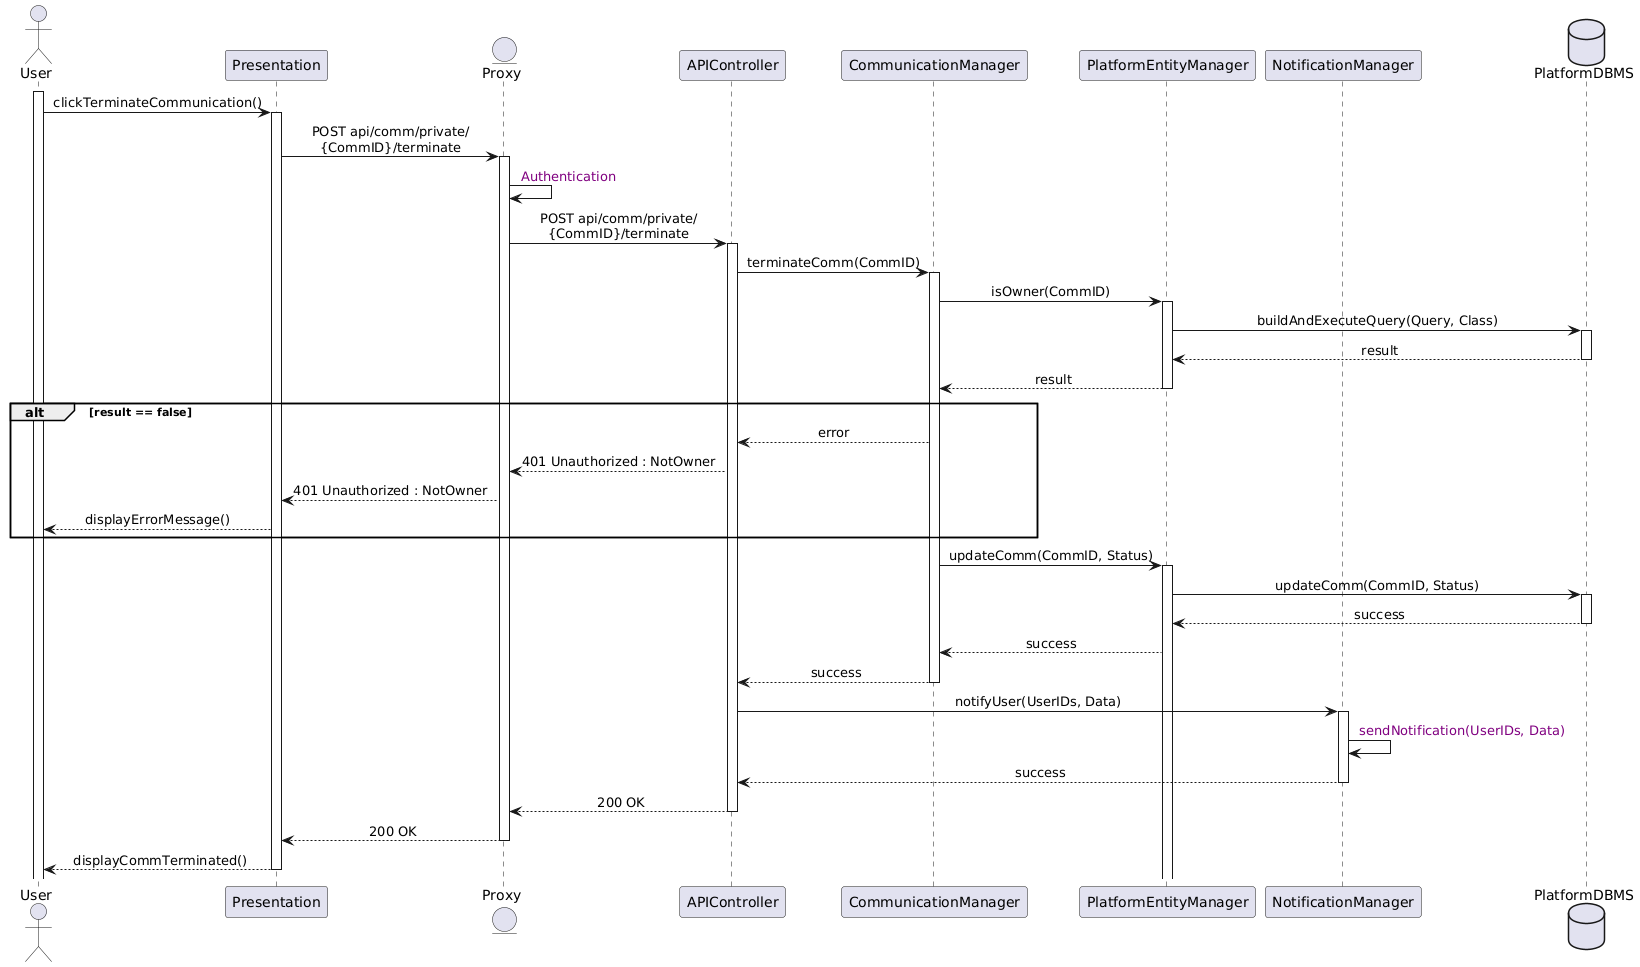
\includegraphics[width=\linewidth]{Latex/Images/DD/SequenceDiagrams/20UserTerminatesCommunication.png}
    \caption{User Terminates Communication Sequence Diagram}
    \label{fig:ustermcomm}
\end{figure}
When the User clicks the "Terminate Communication" button, the Presentation Layer sends a POST private API call to the Proxy.\\
The Proxy authenticates the request and forwards it to the APIController. The APIController calls the CommunicationManager to terminate the specified communication (CommID).\\
The CommunicationManager first verifies if the User is the owner of the communication by querying the PlatformEntityManager. The PlatformEntityManager checks the ownership in the PlatformDBMS and returns the result.\\
If the User is not the owner (result == false), an error message (401 Unauthorized: NotOwner) is returned through the chain to the Presentation Layer, which displays an error message to the User.\\
If the User is the owner, the CommunicationManager updates the communication's status to "terminated" by interacting with the PlatformEntityManager, which performs the update in the PlatformDBMS. Upon success, the update is confirmed back up the chain.\\
The APIController then triggers the NotificationManager to notify all relevant users about the termination of the communication. The NotificationManager sends notifications and confirms their delivery.\\
Finally, the APIController sends a 200 OK response to the Proxy, which forwards it to the Presentation Layer. The Presentation Layer displays a confirmation message to the User indicating that the communication has been successfully terminated.
\subsubsection*{Company Sends an Internship Position Offer}
\begin{figure}[H]
    \centering
    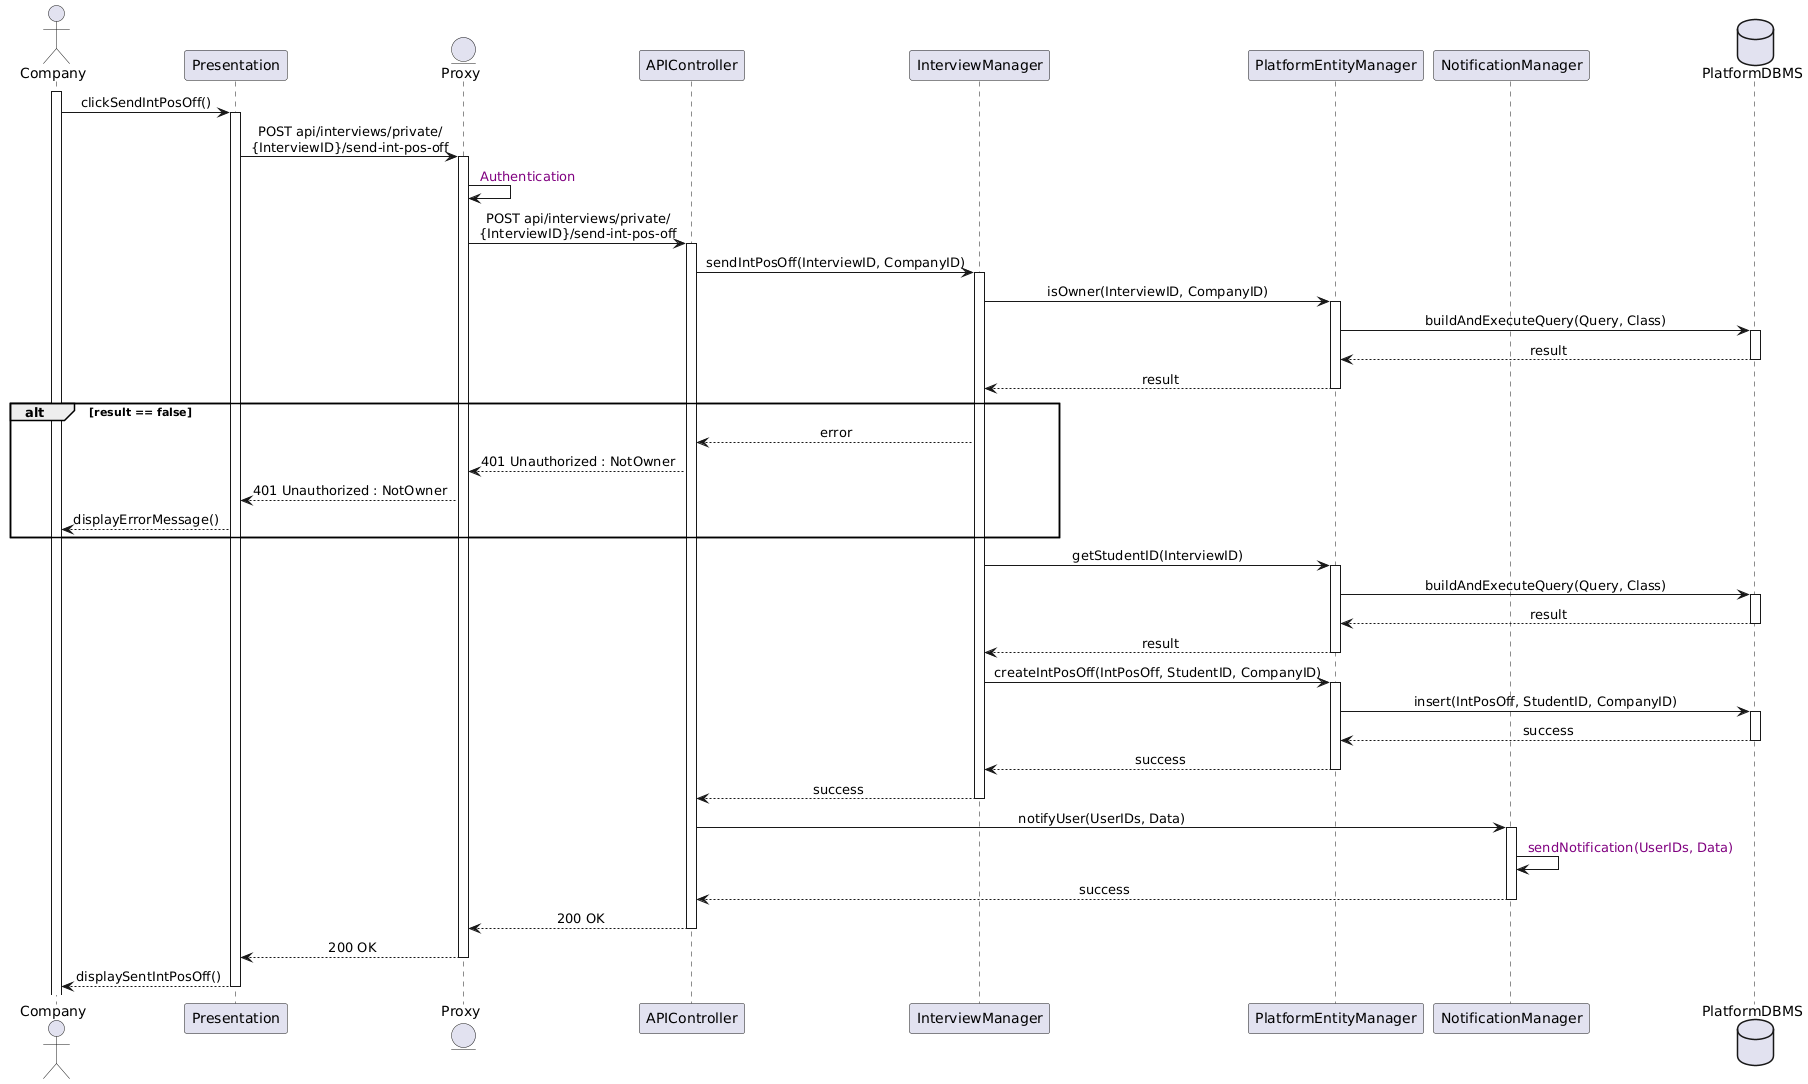
\includegraphics[width=\linewidth]{Latex/Images/DD/SequenceDiagrams/21CompanySendsIntPosOff.png}
    \caption{Company Sends Internship Position Offer Sequence Diagram}
    \label{fig:compsendintposoff}
\end{figure}
When the Company initiates the process to send an internship position offer by clicking the relevant button, the Presentation Layer sends a POST request to the Proxy.

The Proxy authenticates the request and forwards it to the APIController. The APIController invokes the InterviewManager, which first verifies if the Company is the owner of the specified interview by querying the PlatformEntityManager. The PlatformEntityManager communicates with the PlatformDBMS to perform the ownership check.

If the Company is not the owner, an error is returned through the APIController, Proxy, and Presentation Layer, displaying an error message to the Company. If ownership is confirmed, the InterviewManager retrieves the Student ID related to the interview and creates a new internship position offer by interacting with the PlatformEntityManager. The PlatformEntityManager inserts the offer into the database via the PlatformDBMS.

After successfully creating the internship position offer, the InterviewManager returns a success response to the APIController. The APIController then triggers the NotificationManager to notify relevant users about the new offer. Once notifications are sent, the success response propagates back through the Proxy to the Presentation Layer.

Finally, the Presentation Layer displays confirmation of the sent internship position offer to the Company.
% When the Company clicks the "Send Internship Position Offer" button, the Presentation Layer sends a POST private API call to the Proxy.\\
% The Proxy authenticates the request and forwards it to the APIController. The APIController first calls the InterviewManager to verify if the Company is the owner of the interview (InterviewID) by querying the PlatformEntityManager. The PlatformEntityManager checks ownership in the PlatformDBMS and returns the result.\\
% If the Company is not the owner (result == false), an error message (401 Unauthorized: NotOwner) is returned through the chain to the Presentation Layer, which displays an error message to the Company.\\
% If the Company is the owner, the APIController instructs the InterviewManager to proceed with sending the internship position offer. The InterviewManager retrieves the StudentID associated with the InterviewID by querying the PlatformEntityManager.\\
% Once the StudentID is retrieved, the InterviewManager creates the internship position offer (IntPosOff) by inserting it into the PlatformDBMS via the PlatformEntityManager. Upon success, the confirmation is propagated back up the chain.\\
% The APIController then triggers the NotificationManager to notify the relevant student about the offer. The NotificationManager sends notifications and confirms their delivery.\\
% Finally, the APIController sends a 200 OK response to the Proxy, which forwards it to the Presentation Layer. The Presentation Layer displays a confirmation message to the Company, indicating that the internship position offer has been successfully sent.
\subsubsection*{Student Accepts Internship Position Offer}
\begin{figure}[H]
    \centering
    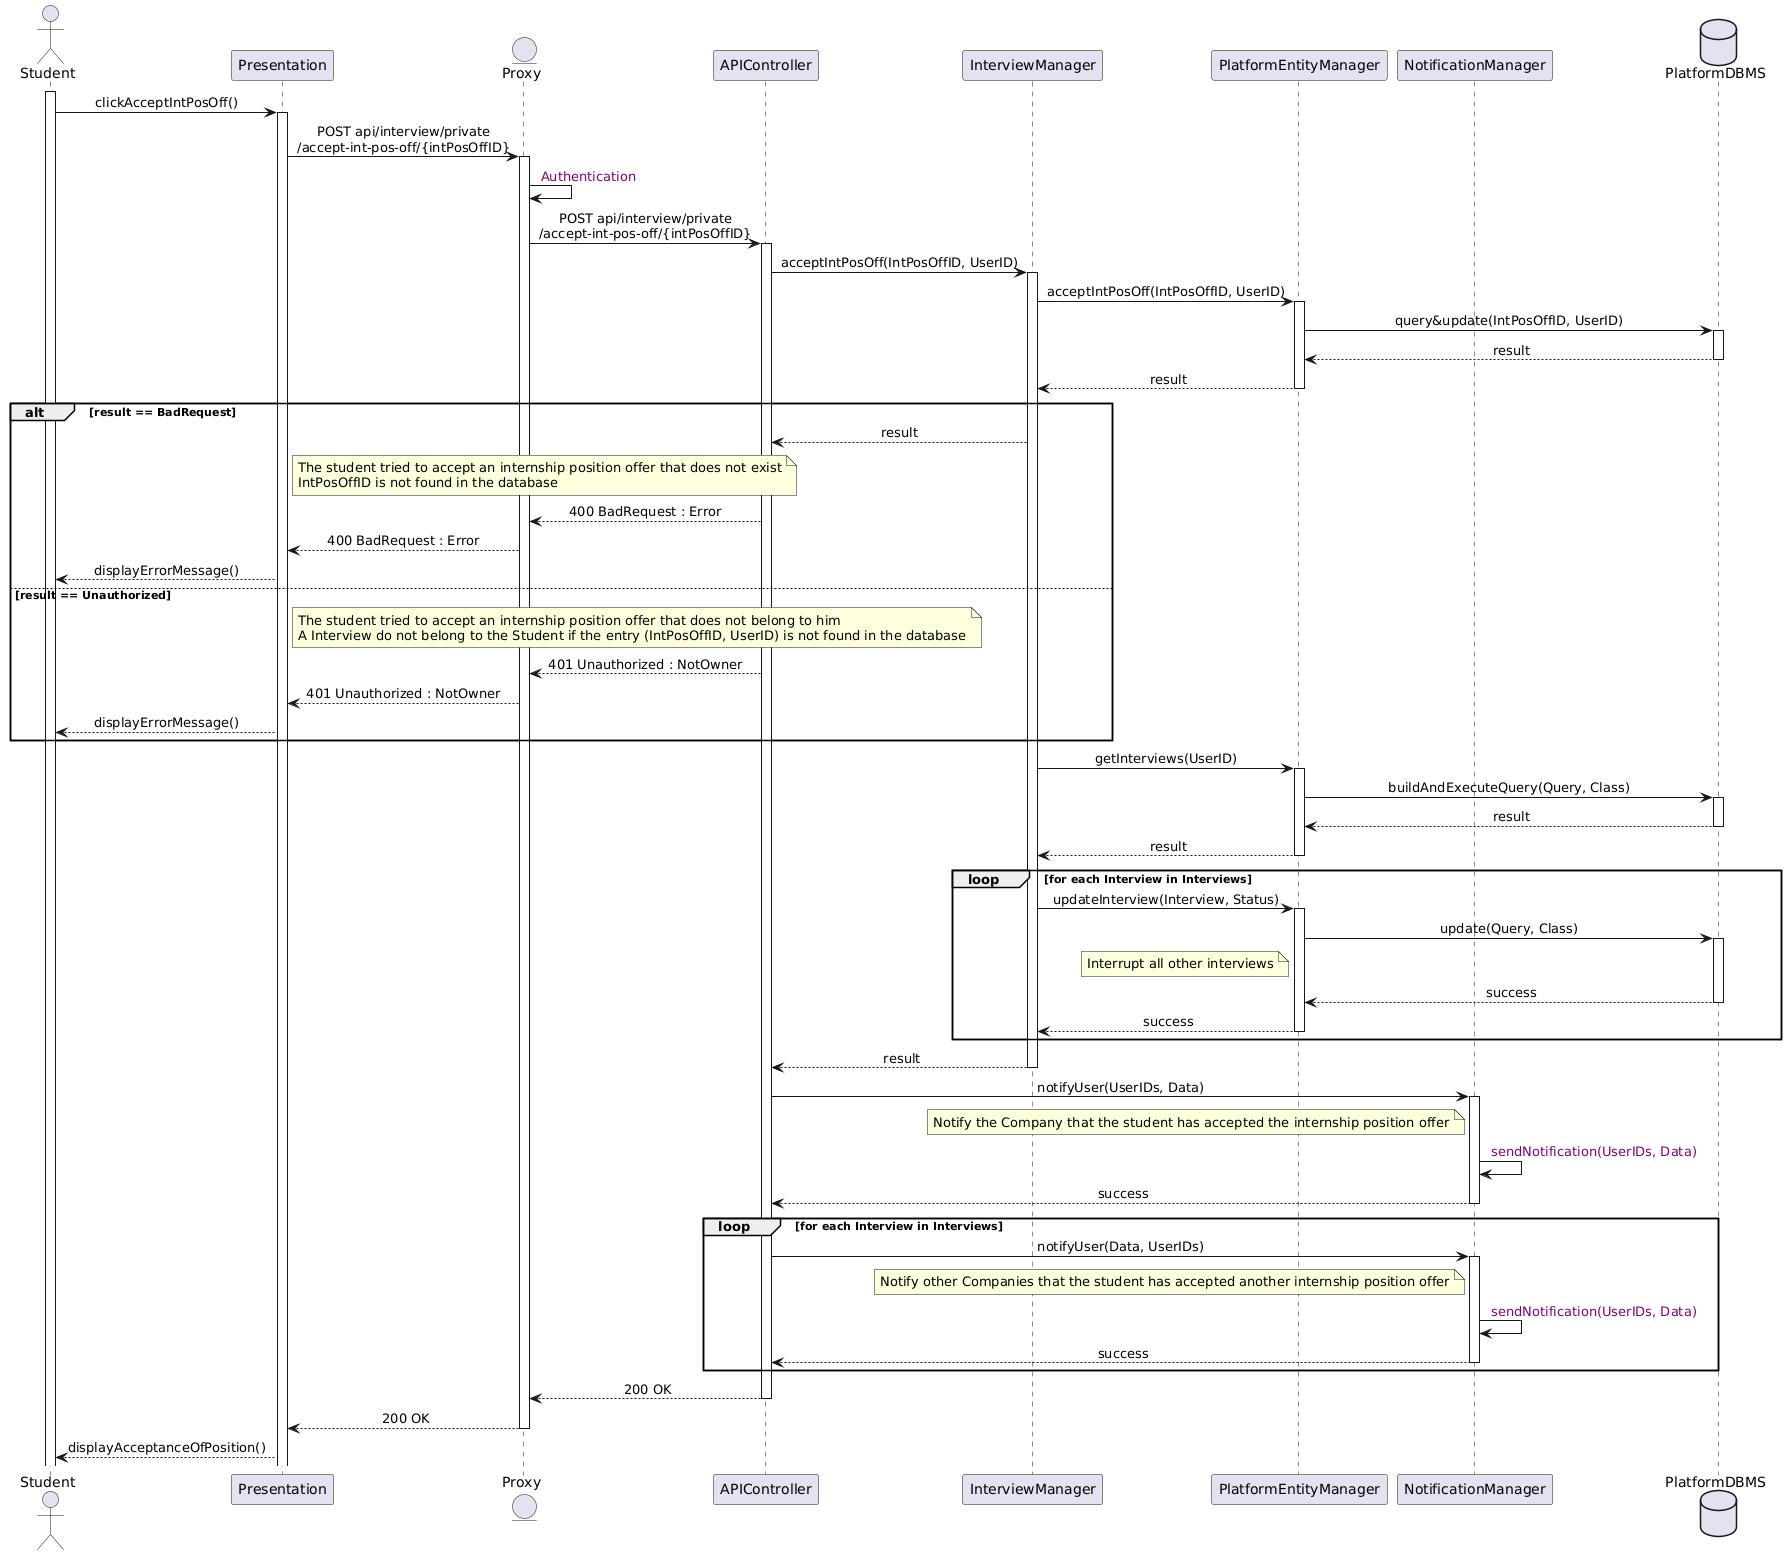
\includegraphics[width=\linewidth]{Latex/Images/DD/SequenceDiagrams/22StudentAcceptsInternshipPositionOffer.png}
    \caption{Student Accepts Internship Position Offer Sequence Diagram}
    \label{fig:studaccintposoff}
\end{figure}
When a Student clicks to accept an internship position offer, the Presentation Layer sends a POST request to the Proxy.\\
The Proxy authenticates the request and forwards it to the APIController. The APIController invokes the InterviewManager to handle the acceptance process. The InterviewManager checks the ownership of the offer by interacting with the PlatformEntityManager, which queries the PlatformDBMS. If the offer does not exist (BadRequest) or does not belong to the Student (Unauthorized), an error response is returned to the Presentation Layer, and an error message is displayed.\\
If the ownership is validated, the InterviewManager retrieves all interviews associated with the Student by querying the PlatformEntityManager. For each of these interviews, the InterviewManager interrupts them by updating their status in the PlatformDBMS.\\
Once all other interviews are updated, the InterviewManager confirms the acceptance of the internship position offer. The APIController triggers the NotificationManager to notify the relevant Company about the Student's acceptance. Additional notifications are sent to other Companies, informing them that the Student has accepted a different offer.\\
Finally, a success response is returned through the Proxy to the Presentation Layer, which displays a confirmation message to the Student.
% When the Student clicks the "Accept Internship Position Offer" button, the Presentation Layer sends a POST private API call to the Proxy.\\
% The Proxy authenticates the request and forwards it to the APIController. The APIController calls the InterviewManager to process the acceptance of the internship position offer (IntPosOffID) for the student (UserID). The InterviewManager uses the PlatformEntityManager to query and update the database entry in PlatformDBMS for the internship position offer.\\
% If the offer does not exist (BadRequest), or the offer does not belong to the student (Unauthorized), an appropriate error is returned through the Proxy to the Presentation Layer, which displays an error message to the student.\\
% If the offer is valid, the APIController triggers the NotificationManager to notify the corresponding company that the student has accepted the internship position offer.\\
% Next, the APIController instructs the InterviewManager to stop any other ongoing interviews for the student. The InterviewManager retrieves all interviews associated with the student from the PlatformEntityManager and updates their status in the PlatformDBMS.\\
% For each canceled interview, the NotificationManager is called to notify the respective companies that the student has accepted another internship position offer.\\
% Finally, a 200 OK response is returned through the Proxy to the Presentation Layer, which displays a confirmation message to the student indicating successful acceptance of the position.
\subsubsection*{Company Sends Template Interview}
\begin{figure}[H]
    \centering
    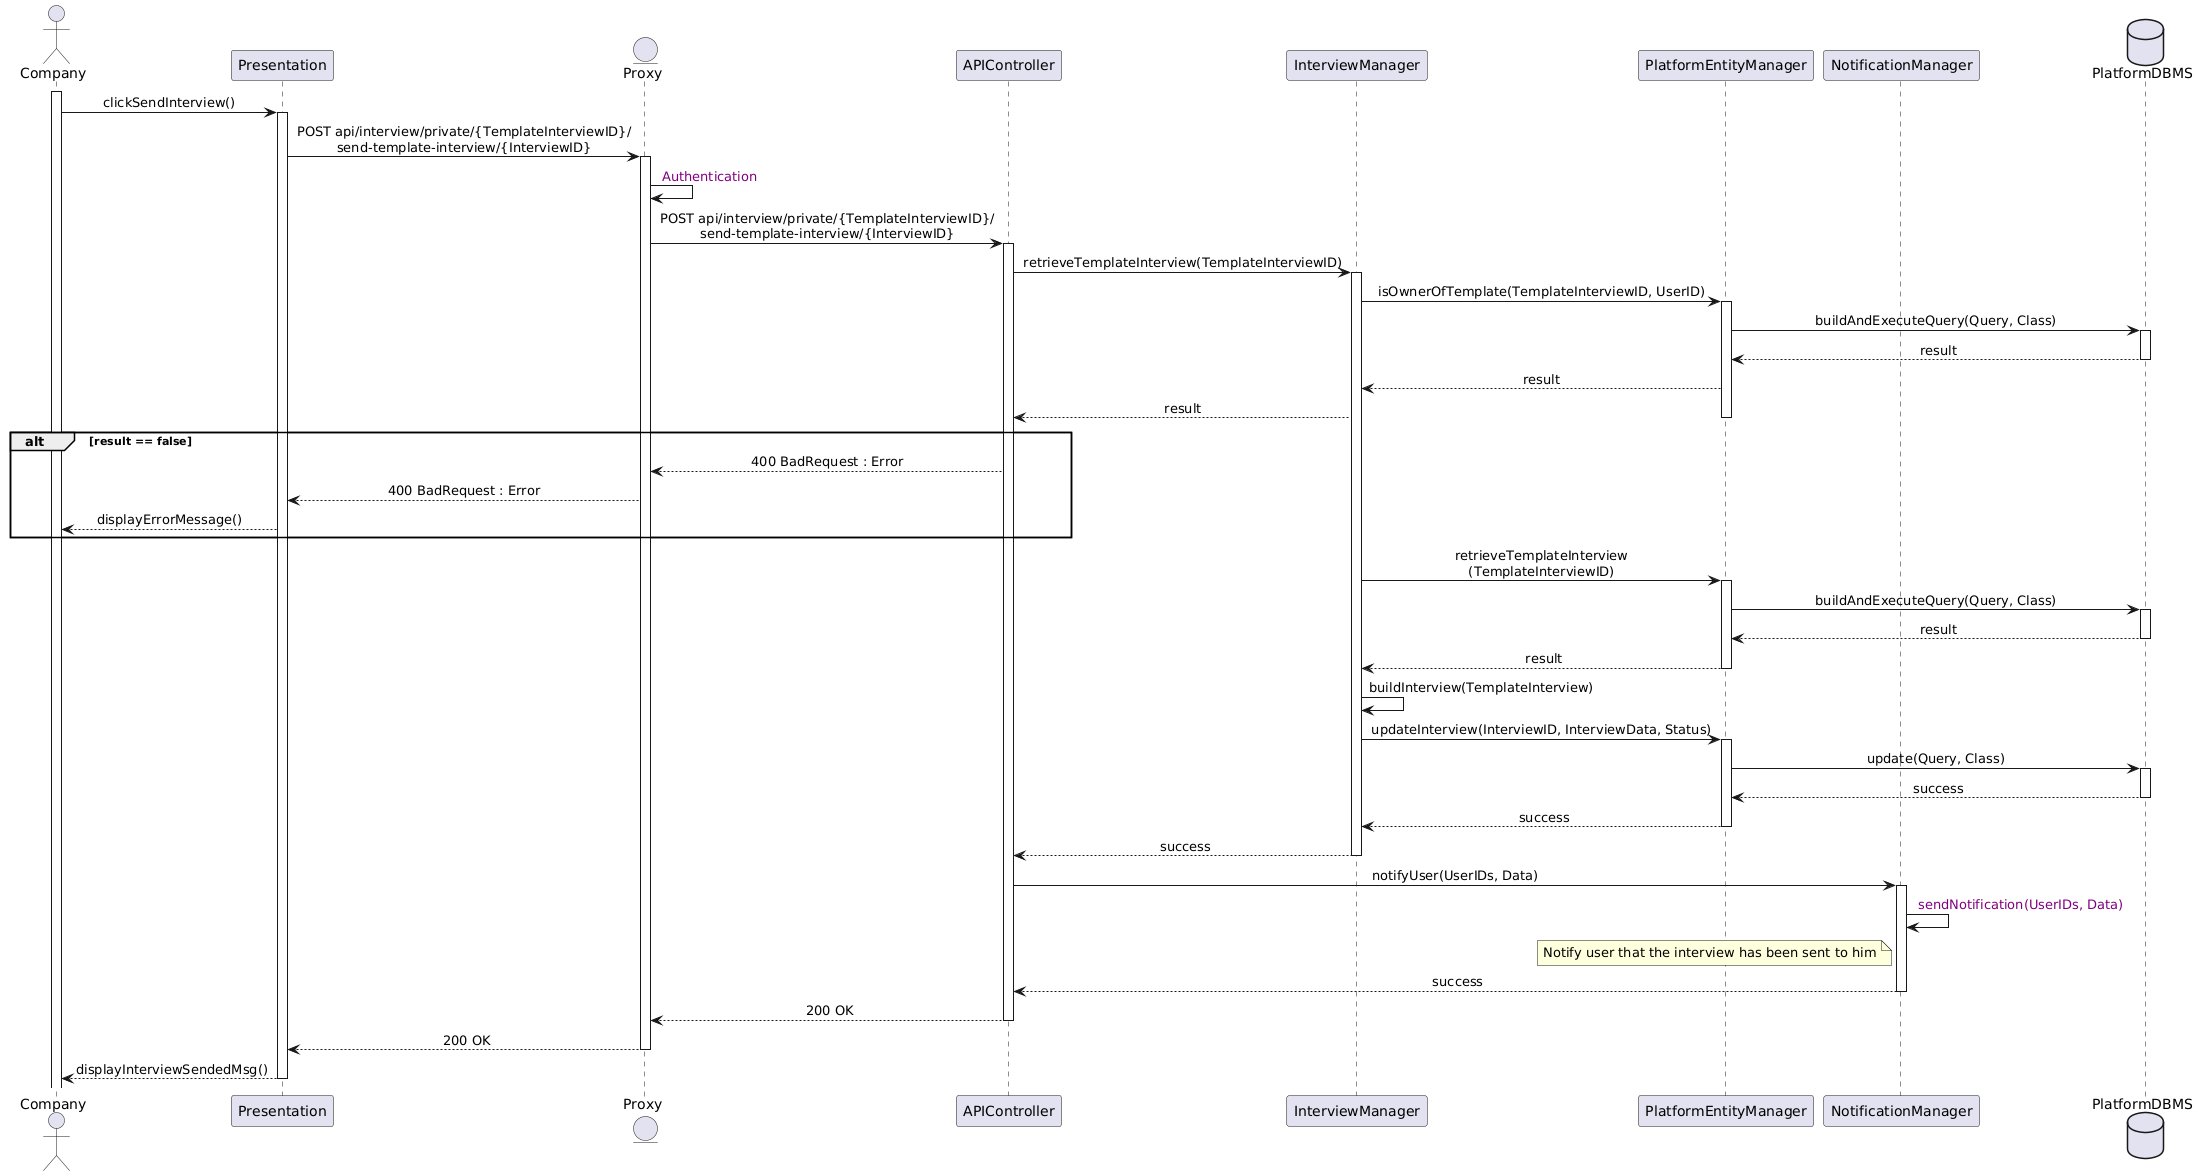
\includegraphics[width=\linewidth]{Latex/Images/DD/SequenceDiagrams/23CompanySendTemplateInterview.png}
    \caption{Company Sends Template Interview Sequence Diagram}
    \label{fig:compsenstempint}
\end{figure}
When a Company clicks to send a saved interview, the Presentation Layer sends a POST request containing the InterviewID and TemplateInterviewID to the Proxy.\\
The Proxy authenticates the request and forwards it to the APIController. The APIController invokes the InterviewManager to retrieve the template interview. The InterviewManager checks if the Company owns the specified template by querying the PlatformEntityManager, which interacts with the PlatformDBMS. If the ownership check fails, an error response is returned, and an error message is displayed to the Company.\\
If the ownership check succeeds, the InterviewManager retrieves the template data from the database and constructs the interview based on the template. The updated interview data is then stored in the database by the PlatformEntityManager.\\
After the interview is successfully updated, the APIController triggers the NotificationManager to notify the Student that the interview has been sent. A success response is then returned through the Proxy to the Presentation Layer, which displays a confirmation message to the Company.
% When a Company clicks the "Send Interview" button, the Presentation Layer sends a POST private API call to the Proxy. The request contains both the TemplateInterviewID and the InterviewID in its body.\\
% The Proxy authenticates the request and forwards it to the APIController. The APIController calls the InterviewManager to verify if the company owns the interview template (TemplateInterviewID). The InterviewManager queries the database through the PlatformEntityManager and PlatformDBMS to validate ownership.\\
% If the result is false, indicating that the company does not own the template, an error (400 BadRequest) is returned to the Presentation Layer, which displays an error message to the company.\\
% If ownership is confirmed, the InterviewManager retrieves the template data associated with the TemplateInterviewID from the database, builds the interview data using the template, and updates the corresponding interview (InterviewID) in the database with the new data and status.\\
% Once the update is successful, the APIController triggers the NotificationManager to notify the user that the interview has been sent to them.\\
% Finally, a 200 OK response is returned through the Proxy to the Presentation Layer, which displays a confirmation message to the company indicating the interview has been successfully sent.

\subsubsection*{Company Closes Internship Offer}
\begin{figure}[H]
    \centering
    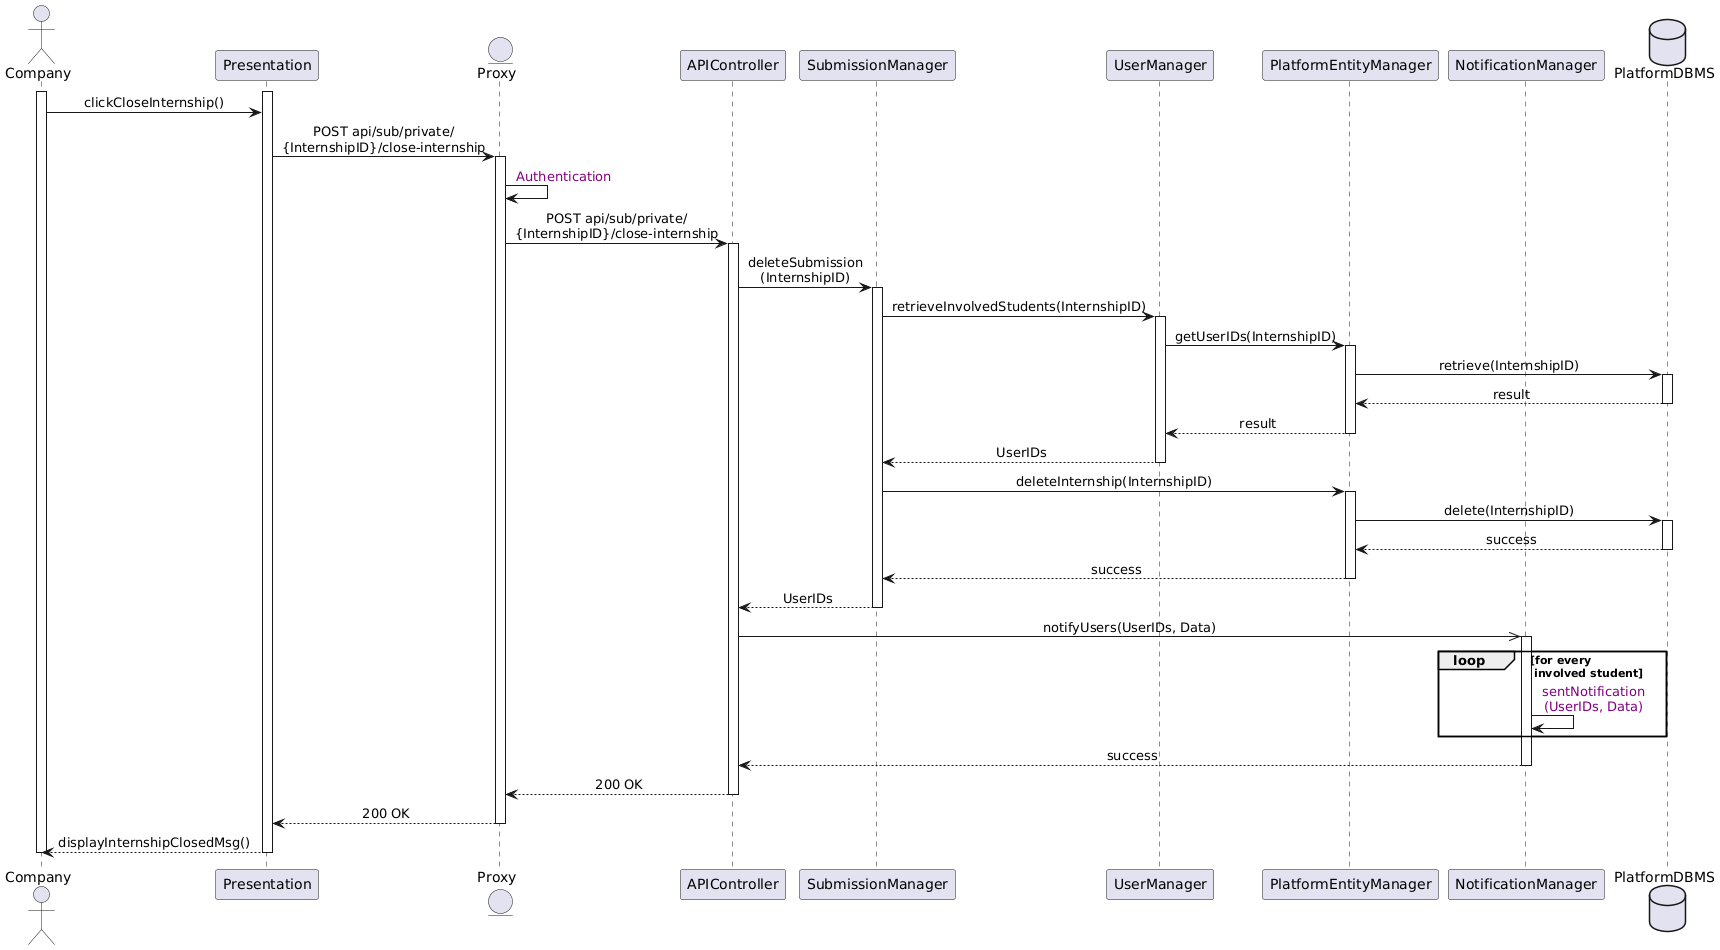
\includegraphics[width=\linewidth]{Latex/Images/DD/SequenceDiagrams/24CompanyClosesInternshipOffer.png}
    \caption{Company Closes Internship Offer Sequence Diagram}
    \label{fig:compclosintoffer}
\end{figure}
When a Company clicks the "Close Internship" button, the Presentation Layer sends a POST private API call to the Proxy. The request contains the InternshipID.\\
The Proxy authenticates the request and forwards it to the APIController. The APIController calls the SubmissionManager to delete the internship submission associated with the InternshipID.\\
The SubmissionManager retrieves the user IDs of all students involved in the internship by querying the UserManager. The UserManager interacts with the database through the PlatformEntityManager and PlatformDBMS to fetch the relevant user IDs.\\
Once the user IDs are retrieved, the SubmissionManager deletes the internship from the database using the PlatformEntityManager and PlatformDBMS.\\
After successfully deleting the internship, the APIController triggers the NotificationManager to notify all involved students about the closure of the internship. Notifications are sent for each user involved in the internship.\\
Finally, a 200 OK response is returned through the Proxy to the Presentation Layer, which displays a confirmation message.


\subsection{Component Interfaces}
In this section, we will outline the interfaces of each component of the S\&C platform. We will detail the methods and parameters they expose, as well as the data they return. The first image provides a general overview of the components, resembling the component view but with a focus on the interfaces between them. The second image offers a more detailed representation of the interfaces within the Platform Logic components, while the third image highlights the interfaces exposed and utilized by the Notification Manager.
In these images, we aimed to illustrate each method exposed by every component. This is why the number of methods depicted here is greater than in the sequence diagrams, where some methods were combined into a single one due to space constraints.
\begin{figure}[H]
    \centering
    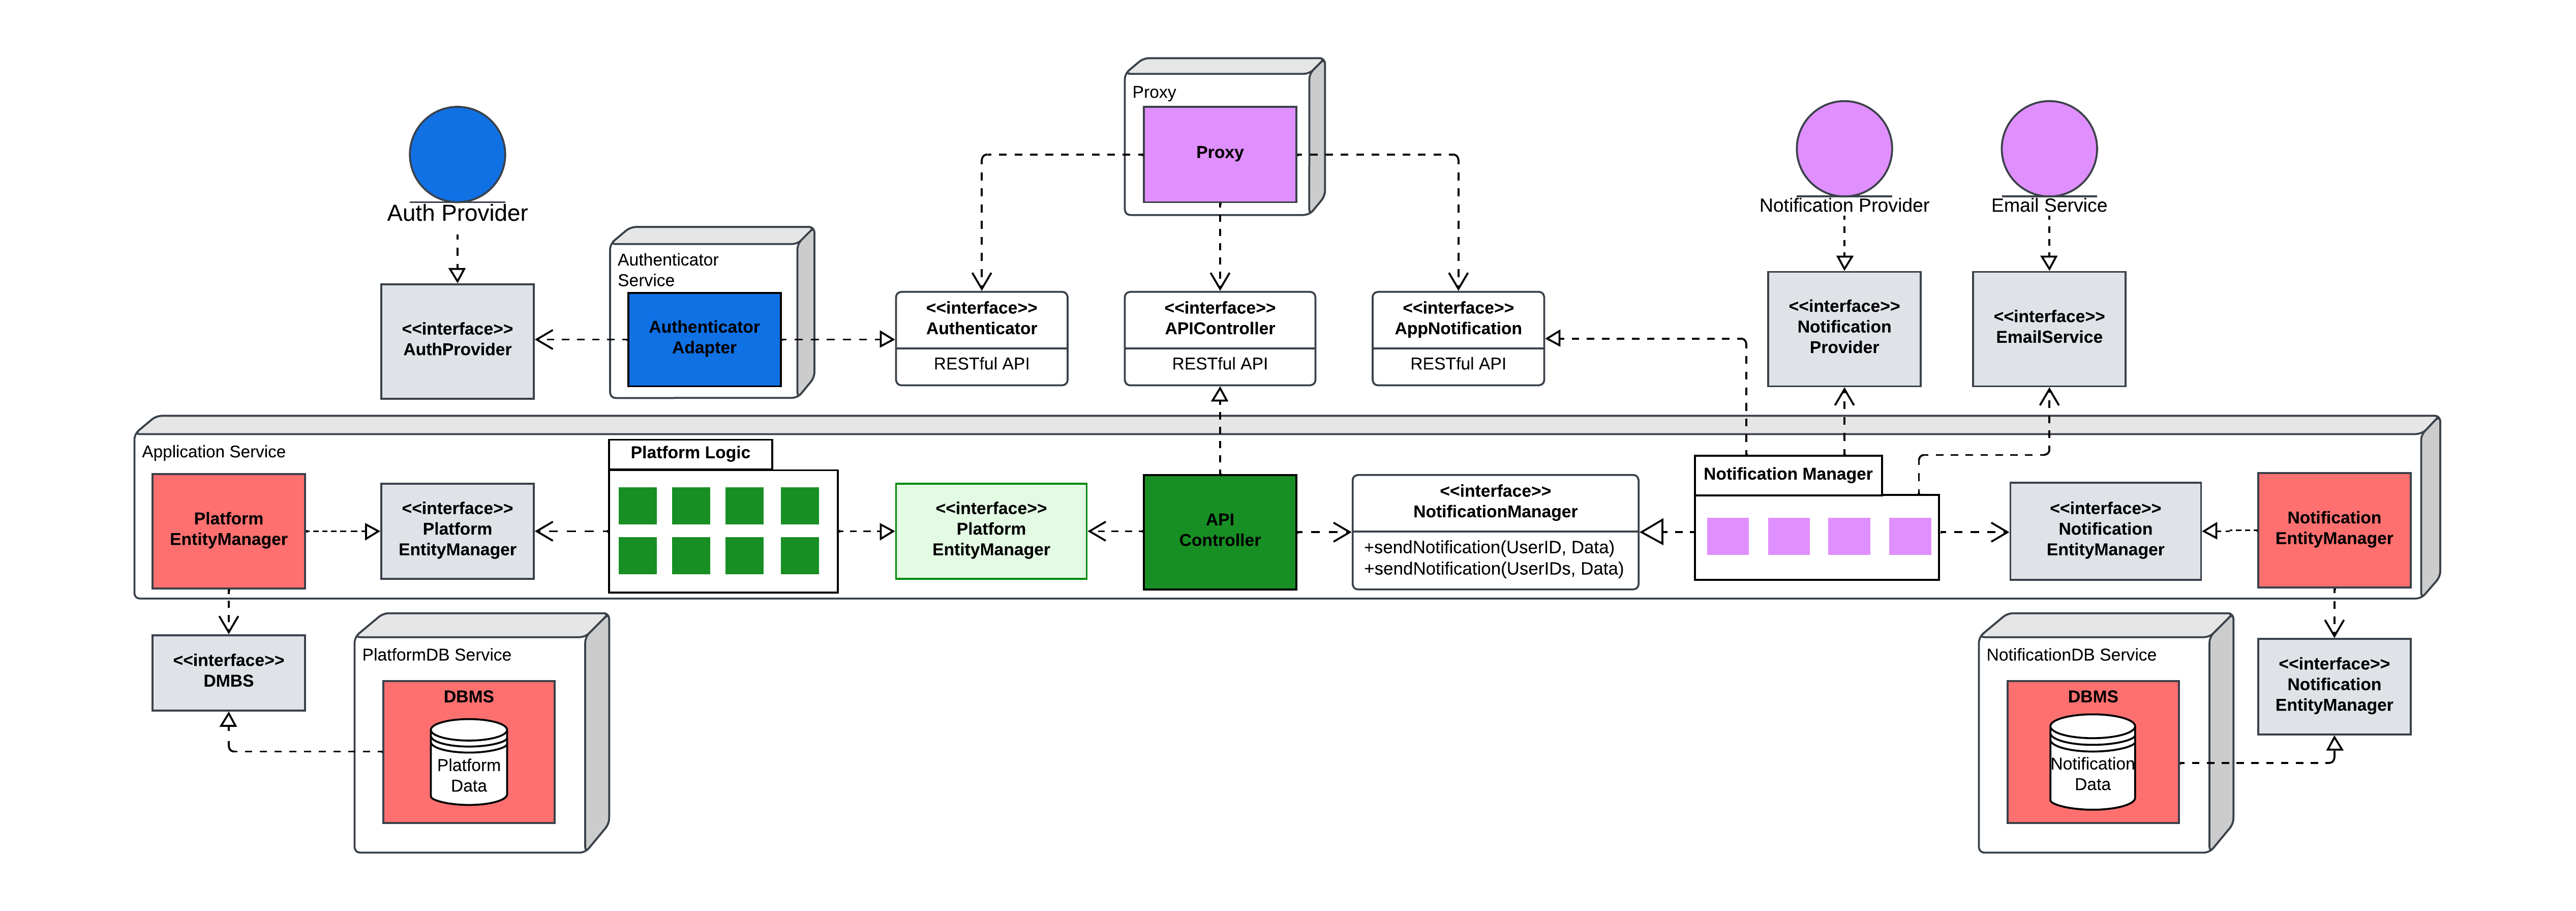
\includegraphics[width=\linewidth]{Latex/Images/DD/Interfaces0.png}
    \caption{Components Interfaces Overview}
    \label{fig:intoverview}
\end{figure}
\begin{figure}[H]
    \centering
    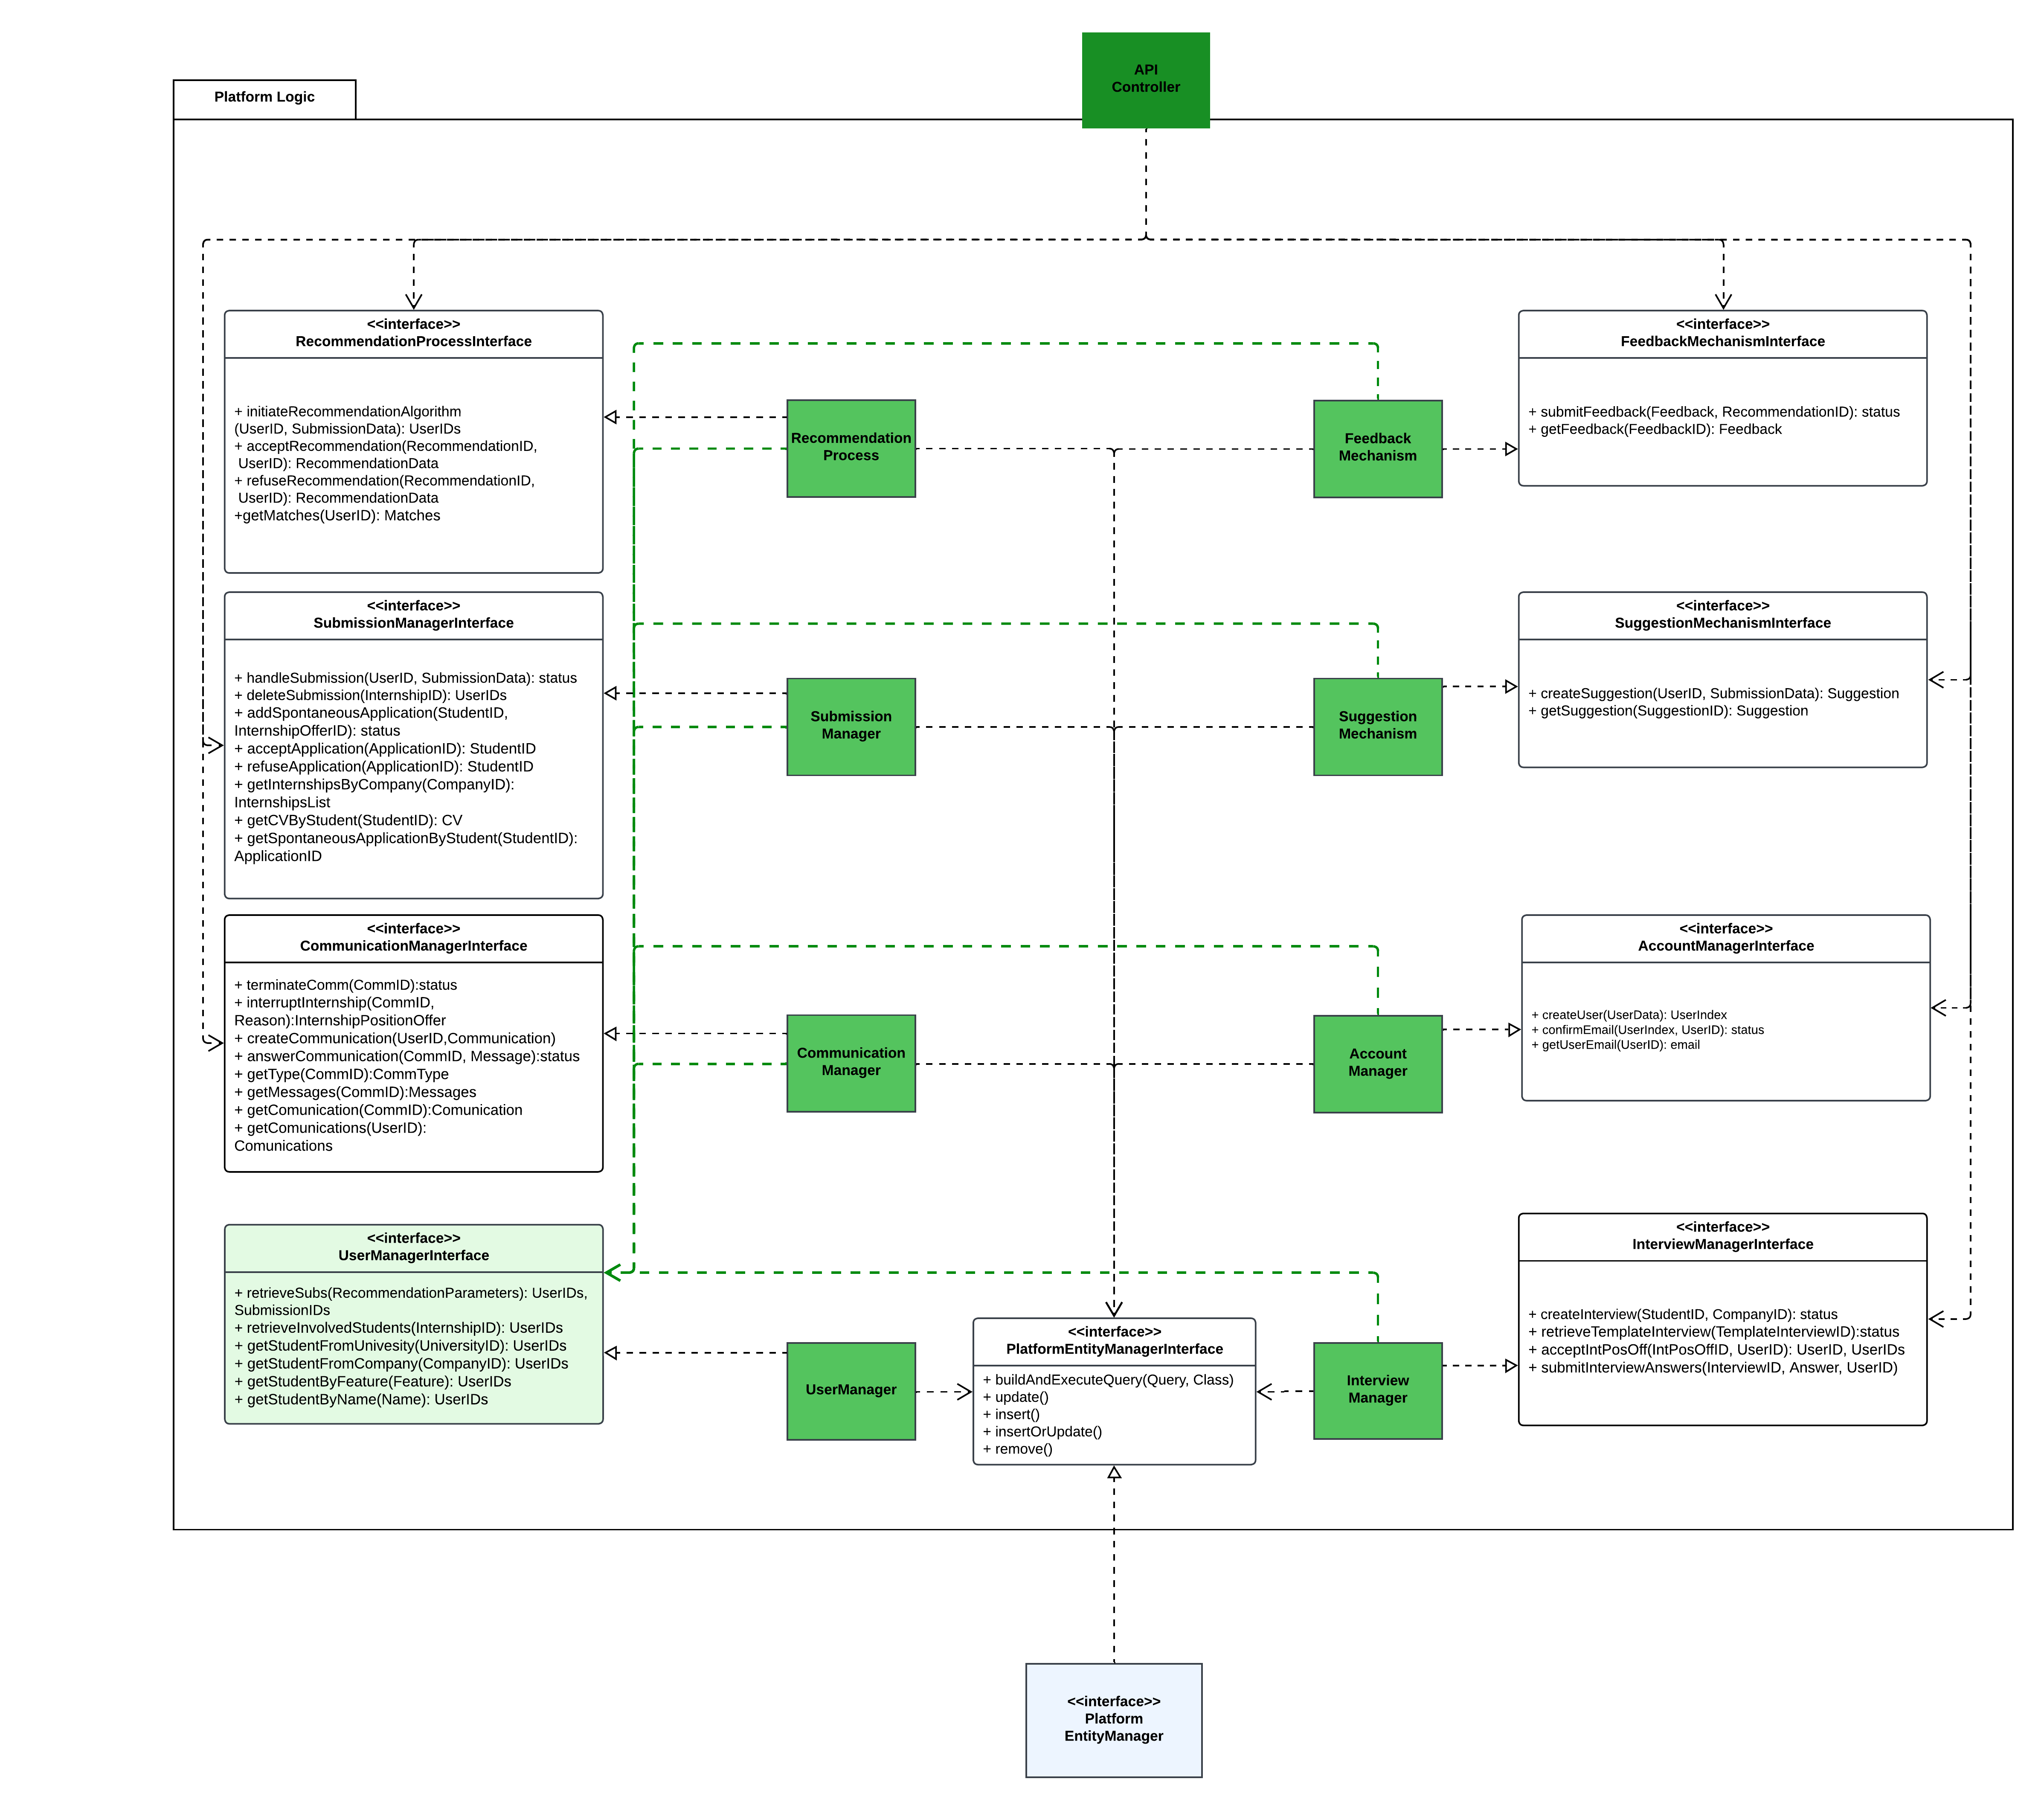
\includegraphics[width=\linewidth]{Latex/Images/DD/Interfaces1.png}
    \caption{Platform Logic Components Interfaces}
    \label{fig:pltcompinterfaces}
\end{figure}
\begin{figure}[H]
    \centering
    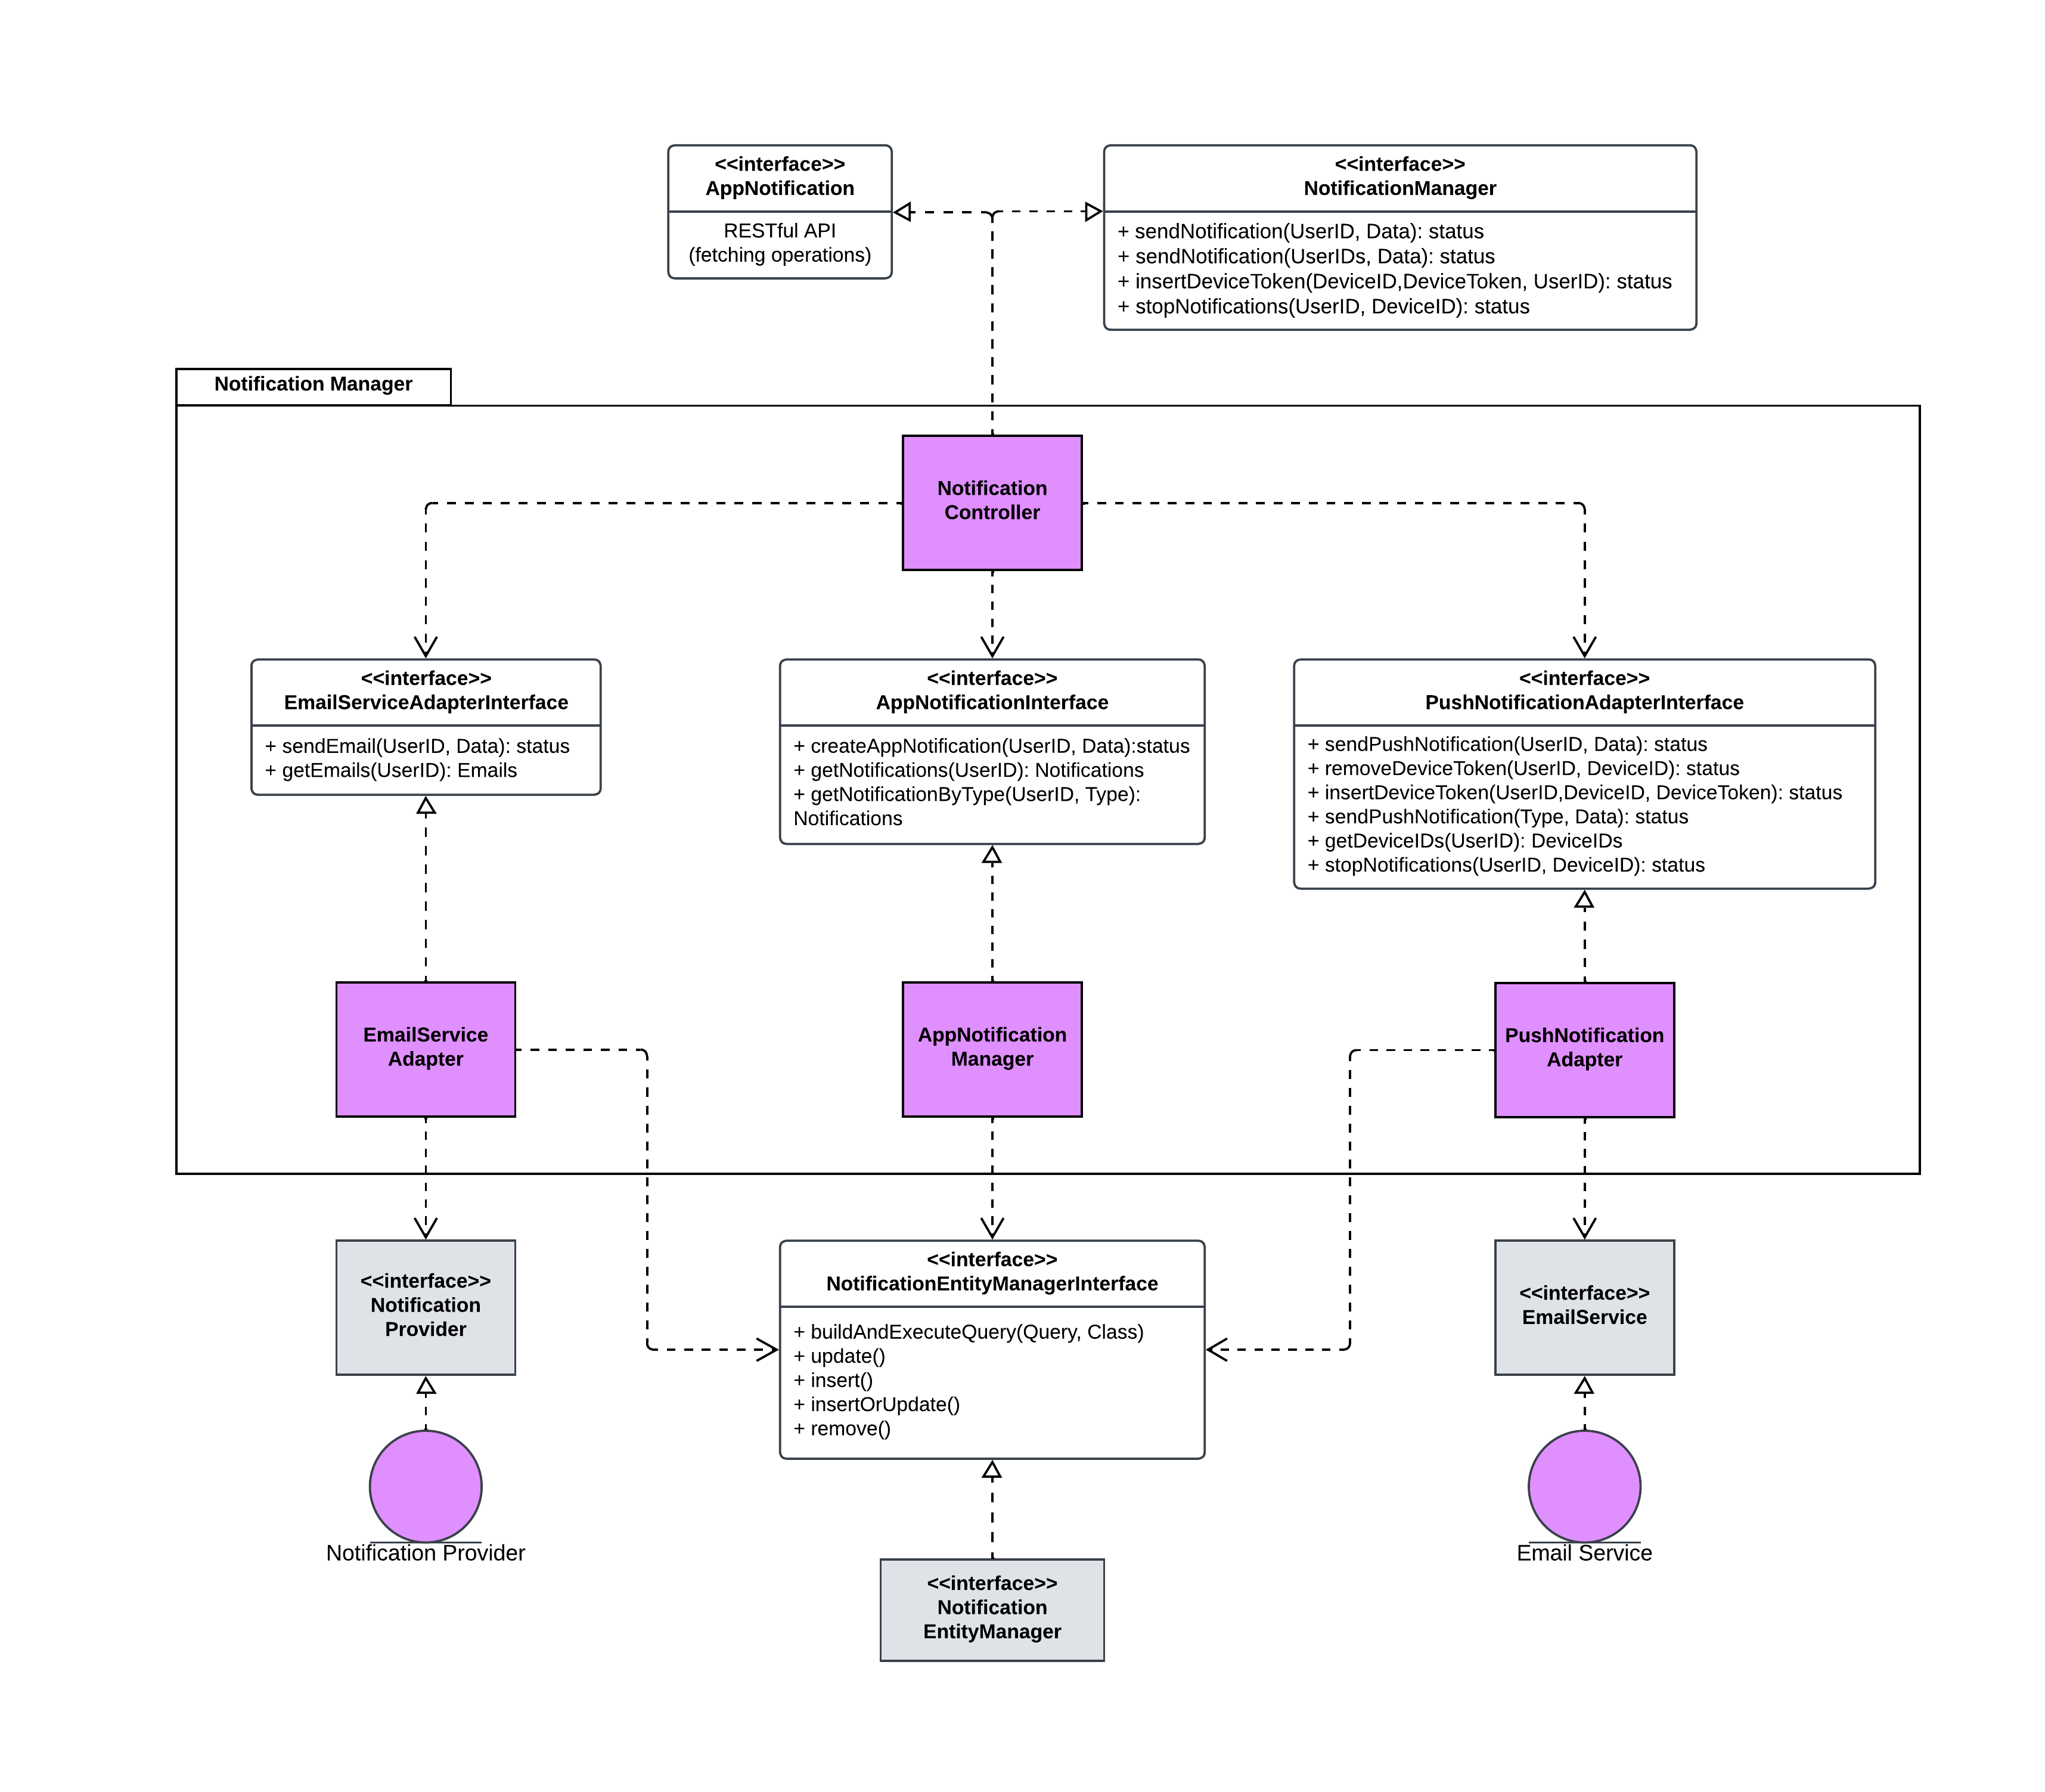
\includegraphics[width=\linewidth]{Latex/Images/DD/Interfaces2.png}
    \caption{Notification Manager Components Interfaces}
    \label{fig:notifyinterfaces}
\end{figure}
\subsubsection{RESTful API endpoints}
\subsubsection*{Proxy Endpoints}
All the calls are routed to the Proxy that handles authentication
redirecting private calls to the Authenticator service. That means that,
in a sense, all the endpoints are Proxy endpoints. The Token to let the user authenticate is added to the header of
the each private request. The Proxy will route the call to the
Authenticator service that will validate the token and return the UserID
to the Proxy that will then route the call to the right service.
However there are some calls to which the Proxy add middleware endpoints that don't
involve the simple token validation procedures, common to all the private
calls. Those particular calls are the ones that follows:\\

\noindent\textbf{\color{titleColor}POST api/auth/login}
\vspace{2pt}
\\\textbf{\color{titleColor}Request Body:} UserCredentials : Object 
\vspace{4pt}
\\\textbf{\color{titleColor}Responses:} 
\begin{itemize}
    \item {\color{titleColor}201 Created:} Token : Object
    \item {\color{titleColor}400 Bad Request:} InvalidError : Object
    \item {\color{titleColor}401 Unauthorized:} UnauthorizedError : Object
    \item {\color{titleColor}500 Internal Server Error:} InternalServerError : Object
\end{itemize}
\textbf{\color{titleColor}Call Stack:} Proxy -> api/auth/validate-credentials -> api/auth/validate-token

\vspace{10pt}
\noindent{\color{titleColor}\rule{0.8\linewidth}{0.2mm}}
\vspace{10pt}

\noindent\textbf{\color{titleColor}POST api/auth/create-token}
\vspace{2pt}
\\\textbf{\color{titleColor}Request Body:} UserCredentials : Object 
\vspace{4pt}
\\\textbf{\color{titleColor}Responses:} 
\begin{itemize}
    \item {\color{titleColor}201 Created:} Token : Object
    \item {\color{titleColor}400 Bad Request:} InvalidError : Object
    \item {\color{titleColor}409 Conflict:} ConflictError : Object
    \item {\color{titleColor}500 Internal Server Error:} InternalServerError : Object
\end{itemize}
\textbf{\color{titleColor}Call Stack:} Proxy -> api/auth/insert-credentials -> api/auth/generate-token

\subsubsection*{Application Endpoints}\label{application-endpoints}

These calls are routed by the Proxy to the Application service that
handles the business logic of the application. If the call has the
private keyword in his address then the Proxy routes it to
\verb|api/auth/validate| middleware to validate the token. That means
that every private call shall contain the Token Object in its body.\\

\noindent\textbf{\color{titleColor}POST api/account/public/register}
\vspace{2pt}
\\\textbf{\color{titleColor}Request Body:} UserData : Object 
\vspace{4pt}
\\\textbf{\color{titleColor}Responses:} 
\begin{itemize}
    \item {\color{titleColor}201 Created:} UserIndex : Object
    \item {\color{titleColor}400 Bad Request:} InvalidError : Object
    \item {\color{titleColor}409 Conflict:} ConflictError : Object
    \item {\color{titleColor}500 Internal Server Error:} InternalServerError : Object
\end{itemize}
\vspace{10pt}
\noindent{\color{titleColor}\rule{0.8\linewidth}{0.2mm}}
\vspace{10pt}

\noindent\textbf{\color{titleColor}POST api/notify/private/send-conf-email}
\vspace{2pt}
\\\textbf{\color{titleColor}Request Body:} UserIndex : Object 
\vspace{4pt}
\\\textbf{\color{titleColor}Responses:} 
\begin{itemize}
    \item {\color{titleColor}201 Created:} Message : Object
    \item {\color{titleColor}400 Bad Request:} InvalidError : Object
    \item {\color{titleColor}401 Unauthorized:} UnauthorizedError : Object
    \item {\color{titleColor}500 Internal Server Error:} InternalServerError : Object
\end{itemize}
\vspace{10pt}
\noindent{\color{titleColor}\rule{0.8\linewidth}{0.2mm}}
\vspace{10pt}

\noindent\textbf{\color{titleColor}POST api/notify/private/conf-email}
\vspace{2pt}
\\\textbf{\color{titleColor}Responses:} 
\begin{itemize}
    \item {\color{titleColor}200 OK}
    \item {\color{titleColor}400 Bad Request:} InvalidError : Object
    \item {\color{titleColor}401 Unauthorized:} UnauthorizedError : Object
    \item {\color{titleColor}500 Internal Server Error:} InternalServerError : Object
\end{itemize}
\vspace{10pt}
\noindent{\color{titleColor}\rule{0.8\linewidth}{0.2mm}}
\vspace{10pt}

\noindent\textbf{\color{titleColor}POST api/sub/private/update-sub}
\vspace{2pt}
\\\textbf{\color{titleColor}Request Body:} SubmissionData : Object 
\vspace{4pt}
\\\textbf{\color{titleColor}Responses:} 
\begin{itemize}
    \item {\color{titleColor}201 Created:} SubmissionID, Suggestions : Object
    \item {\color{titleColor}400 Bad Request:} InvalidError : Object
    \item {\color{titleColor}401 Unauthorized:} UnauthorizedError : Object
    \item {\color{titleColor}409 Conflict:} ConflictError : Object
    \item {\color{titleColor}500 Internal Server Error:} InternalServerError : Object
\end{itemize}
\vspace{10pt}
\noindent{\color{titleColor}\rule{0.8\linewidth}{0.2mm}}
\vspace{10pt}

\noindent\textbf{\color{titleColor}GET api/sub/private/internships/\{CompanyID\}}
\vspace{2pt}
\\\textbf{\color{titleColor}Responses:} 
\begin{itemize}
    \item {\color{titleColor}200 OK:} InternshipsList : Object
    \item {\color{titleColor}400 Bad Request:} InvalidError : Object
    \item {\color{titleColor}401 Unauthorized:} UnauthorizedError : Object
    \item {\color{titleColor}409 Conflict:} ConflictError : Object
    \item {\color{titleColor}500 Internal Server Error:} InternalServerError : Object
\end{itemize}
\vspace{10pt}
\noindent{\color{titleColor}\rule{0.8\linewidth}{0.2mm}}
\vspace{10pt}

\noindent\textbf{\color{titleColor}GET api/sub/private/cv/\{StudentID\}}
\vspace{2pt}
\\\textbf{\color{titleColor}Responses:} 
\begin{itemize}
    \item {\color{titleColor}200 OK:} CV : Object
    \item {\color{titleColor}400 Bad Request:} InvalidError : Object
    \item {\color{titleColor}401 Unauthorized:} UnauthorizedError : Object
    \item {\color{titleColor}409 Conflict:} ConflictError : Object
    \item {\color{titleColor}500 Internal Server Error:} InternalServerError : Object
\end{itemize}
\vspace{10pt}
\noindent{\color{titleColor}\rule{0.8\linewidth}{0.2mm}}
\vspace{10pt}

\noindent\textbf{\color{titleColor}POST api/recommendations/private/\{RecommendationID\}/accept}
\vspace{2pt}
\\\textbf{\color{titleColor}Responses:} 
\begin{itemize}
    \item {\color{titleColor}201 Created:} 
    \begin{itemize}
        \item askFeedback : Object
        \item Message : Object
    \end{itemize}
    \item {\color{titleColor}400 Bad Request:} InvalidError : Object
    \item {\color{titleColor}401 Unauthorized:} UnauthorizedError : Object
    \item {\color{titleColor}409 Conflict:} ConflictError : Object
    \item {\color{titleColor}500 Internal Server Error:} InternalServerError : Object
\end{itemize}
\vspace{10pt}
\noindent{\color{titleColor}\rule{0.8\linewidth}{0.2mm}}
\vspace{10pt}

\noindent\textbf{\color{titleColor}PUT api/feedback/private/\{RecommendationID\}/submit}
\vspace{2pt}
\\\textbf{\color{titleColor}Request Body:} Feedback : Object 
\vspace{4pt}
\\\textbf{\color{titleColor}Responses:} 
\begin{itemize}
    \item {\color{titleColor}200 OK:} Message : Object
    \item {\color{titleColor}400 Bad Request:} InvalidError : Object
    \item {\color{titleColor}401 Unauthorized:} UnauthorizedError : Object
    \item {\color{titleColor}500 Internal Server Error:} InternalServerError : Object
\end{itemize}
\vspace{10pt}
\noindent{\color{titleColor}\rule{0.8\linewidth}{0.2mm}}
\vspace{10pt}

\noindent\textbf{\color{titleColor}POST api/sub/private/application/\{CompanyID\}}
\vspace{2pt}
\\\textbf{\color{titleColor}Responses:} 
\begin{itemize}
    \item {\color{titleColor}200 OK:} Message : Object
    \item {\color{titleColor}400 Bad Request:} InvalidError : Object
    \item {\color{titleColor}401 Unauthorized:} UnauthorizedError : Object
    \item {\color{titleColor}409 Conflict:} ConflictError : Object
    \item {\color{titleColor}500 Internal Server Error:} InternalServerError : Object
\end{itemize}
\vspace{10pt}
\noindent{\color{titleColor}\rule{0.8\linewidth}{0.2mm}}
\vspace{10pt}

\noindent\textbf{\color{titleColor}POST api/comm/private/application/\{ApplicationID\}/accept}
\vspace{2pt}
\\\textbf{\color{titleColor}Responses:} 
\begin{itemize}
    \item {\color{titleColor}200 OK:} Message : Object
    \item {\color{titleColor}400 Bad Request:} InvalidError : Object
    \item {\color{titleColor}401 Unauthorized:} UnauthorizedError : Object
    \item {\color{titleColor}409 Conflict:} ConflictError : Object
    \item {\color{titleColor}500 Internal Server Error:} InternalServerError : Object
\end{itemize}
\vspace{10pt}
\noindent{\color{titleColor}\rule{0.8\linewidth}{0.2mm}}
\vspace{10pt}

\noindent\textbf{\color{titleColor}POST api/interviews/private/send-answer/\{InterviewID\}}
\vspace{2pt}
\\\textbf{\color{titleColor}Request Body:} Answer : Object 
\vspace{4pt}
\\\textbf{\color{titleColor}Responses:} 
\begin{itemize}
    \item {\color{titleColor}200 OK:} Message : Object
    \item {\color{titleColor}400 Bad Request:} InvalidError : Object
    \item {\color{titleColor}401 Unauthorized:} UnauthorizedError : Object
    \item {\color{titleColor}500 Internal Server Error:} InternalServerError : Object
\end{itemize}
\vspace{10pt}
\noindent{\color{titleColor}\rule{0.8\linewidth}{0.2mm}}
\vspace{10pt}

\noindent\textbf{\color{titleColor}POST api/interviews/private/send-interview/\{InterviewID\}}
\vspace{2pt}
\\\textbf{\color{titleColor}Request Body:} InterviewTemplate : Object 
\vspace{4pt}
\\\textbf{\color{titleColor}Responses:} 
\begin{itemize}
    \item {\color{titleColor}201 Created:} Message : Object
    \item {\color{titleColor}400 Bad Request:} InvalidError : Object
    \item {\color{titleColor}401 Unauthorized:} UnauthorizedError : Object
    \item {\color{titleColor}409 Conflict:} ConflictError : Object
    \item {\color{titleColor}500 Internal Server Error:} InternalServerError : Object
\end{itemize}
\vspace{10pt}
\noindent{\color{titleColor}\rule{0.8\linewidth}{0.2mm}}
\vspace{10pt}

\noindent\textbf{\color{titleColor}POST api/interviews/private/save-template-interview/\{InterviewID\}}
\vspace{2pt}
\\\textbf{\color{titleColor}Request Body:} InterviewTemplate : Object 
\vspace{4pt}
\\\textbf{\color{titleColor}Responses:} 
\begin{itemize}
    \item {\color{titleColor}201 Created:} Message : Object
    \item {\color{titleColor}400 Bad Request:} InvalidError : Object
    \item {\color{titleColor}401 Unauthorized:} UnauthorizedError : Object
    \item {\color{titleColor}409 Conflict:} ConflictError : Object
    \item {\color{titleColor}500 Internal Server Error:} InternalServerError : Object
\end{itemize}
\vspace{10pt}
\noindent{\color{titleColor}\rule{0.8\linewidth}{0.2mm}}
\vspace{10pt}

\noindent\textbf{\color{titleColor}POST api/interviews/private/\{TemplateInterviewID\}/send-template-interview/\{InterviewID\}}
\vspace{2pt}
\\\textbf{\color{titleColor}Responses:} 
\begin{itemize}
    \item {\color{titleColor}200 OK:} Message : Object
    \item {\color{titleColor}400 Bad Request:} InvalidError : Object
    \item {\color{titleColor}401 Unauthorized:} UnauthorizedError : Object
    \item {\color{titleColor}409 Conflict:} ConflictError : Object
    \item {\color{titleColor}500 Internal Server Error:} InternalServerError : Object
\end{itemize}
\vspace{10pt}
\noindent{\color{titleColor}\rule{0.8\linewidth}{0.2mm}}
\vspace{10pt}

\noindent\textbf{\color{titleColor}POST api/interviews/private/evaluate-interview/\{InterviewID\}}
\vspace{2pt}
\\\textbf{\color{titleColor}Request Body:} Evaluation : Object 
\vspace{4pt}
\\\textbf{\color{titleColor}Responses:} 
\begin{itemize}
    \item {\color{titleColor}201 Created:} Message : Object
    \item {\color{titleColor}400 Bad Request:} InvalidError : Object
    \item {\color{titleColor}401 Unauthorized:} UnauthorizedError : Object
    \item {\color{titleColor}409 Conflict:} ConflictError : Object
    \item {\color{titleColor}500 Internal Server Error:} InternalServerError : Object
\end{itemize}
\vspace{10pt}
\noindent{\color{titleColor}\rule{0.8\linewidth}{0.2mm}}
\vspace{10pt}

\noindent\textbf{\color{titleColor}GET api/applications/private/get-spontaneous-applications}
\vspace{2pt}
\\\textbf{\color{titleColor}Responses:} 
\begin{itemize}
    \item {\color{titleColor}200 OK:} Applications : Object
    \item {\color{titleColor}400 Bad Request:} InvalidError : Object
    \item {\color{titleColor}401 Unauthorized:} UnauthorizedError : Object
    \item {\color{titleColor}500 Internal Server Error:} InternalServerError : Object
\end{itemize}
\vspace{10pt}
\noindent{\color{titleColor}\rule{0.8\linewidth}{0.2mm}}
\vspace{10pt}

\noindent\textbf{\color{titleColor}GET api/applications/private/get-matches}
\vspace{2pt}
\\\textbf{\color{titleColor}Responses:} 
\begin{itemize}
    \item {\color{titleColor}200 OK:} Matches
    \item {\color{titleColor}400 Bad Request:} InvalidError
    \item {\color{titleColor}401 Unauthorized:} UnauthorizedError
    \item {\color{titleColor}500 Internal Server Error:} InternalServerError
\end{itemize}
\vspace{10pt}
\noindent{\color{titleColor}\rule{0.8\linewidth}{0.2mm}}
\vspace{10pt}

\noindent\textbf{\color{titleColor}POST api/comm/private/\{commID\}/answer}
\vspace{2pt}
\\\textbf{\color{titleColor}Request Body:} Message : Object 
\vspace{4pt}
\\\textbf{\color{titleColor}Responses:} 
\begin{itemize}
    \item {\color{titleColor}201 Created:} Message : Object
    \item {\color{titleColor}400 Bad Request:} InvalidError : Object
    \item {\color{titleColor}401 Unauthorized:} UnauthorizedError : Object
    \item {\color{titleColor}409 Conflict:} ConflictError : Object
    \item {\color{titleColor}500 Internal Server Error:} InternalServerError : Object
\end{itemize}
\vspace{10pt}
\noindent{\color{titleColor}\rule{0.8\linewidth}{0.2mm}}
\vspace{10pt}

\noindent\textbf{\color{titleColor}GET api/comm/private/communications/\{CommID\}}
\vspace{2pt}
\\\textbf{\color{titleColor}Responses:} 
\begin{itemize}
    \item {\color{titleColor}200 OK:} Result : Object
    \item {\color{titleColor}400 Bad Request:} InvalidError : Object
    \item {\color{titleColor}401 Unauthorized:} UnauthorizedError : Object
    \item {\color{titleColor}500 Internal Server Error:} InternalServerError : Object
\end{itemize}
\vspace{10pt}
\noindent{\color{titleColor}\rule{0.8\linewidth}{0.2mm}}
\vspace{10pt}

\noindent\textbf{\color{titleColor}POST api/comm/private/create}
\vspace{2pt}
\\\textbf{\color{titleColor}Request Body:} Communication : Object 
\vspace{4pt}
\\\textbf{\color{titleColor}Responses:} 
\begin{itemize}
    \item {\color{titleColor}201 Created:} Message : Object
    \item {\color{titleColor}400 Bad Request:} InvalidError : Object
    \item {\color{titleColor}401 Unauthorized:} UnauthorizedError : Object
    \item {\color{titleColor}500 Internal Server Error:} InternalServerError : Object
\end{itemize}
\vspace{10pt}
\noindent{\color{titleColor}\rule{0.8\linewidth}{0.2mm}}
\vspace{10pt}

\noindent\textbf{\color{titleColor}GET api/comm/private/communications}
\vspace{2pt}
\\\textbf{\color{titleColor}Responses:} 
\begin{itemize}
    \item {\color{titleColor}200 OK:} Communications : Object
    \item {\color{titleColor}401 Unauthorized:} UnauthorizedError : Object
    \item {\color{titleColor}500 Internal Server Error:} InternalServerError : Object
\end{itemize}
\vspace{10pt}
\noindent{\color{titleColor}\rule{0.8\linewidth}{0.2mm}}
\vspace{10pt}

\noindent\textbf{\color{titleColor}POST api/comm/private/\{commID\}/interrupt-internship}
\vspace{2pt}
\\\textbf{\color{titleColor}Request Body:} Reason : Object 
\vspace{4pt}
\\\textbf{\color{titleColor}Responses:} 
\begin{itemize}
    \item {\color{titleColor}200 OK:} Message : Object
    \item {\color{titleColor}400 Bad Request:} InvalidError : Object
    \item {\color{titleColor}401 Unauthorized:} UnauthorizedError : Object
    \item {\color{titleColor}409 Conflict:} ConflictError : Object
    \item {\color{titleColor}500 Internal Server Error:} InternalServerError : Object
\end{itemize}
\vspace{10pt}
\noindent{\color{titleColor}\rule{0.8\linewidth}{0.2mm}}
\vspace{10pt}

\noindent\textbf{\color{titleColor}POST api/comm/private/\{commID\}/terminate}
\vspace{2pt}
\\\textbf{\color{titleColor}Responses:} 
\begin{itemize}
    \item {\color{titleColor}200 OK:} Message : Object
    \item {\color{titleColor}400 Bad Request:} InvalidError : Object
    \item {\color{titleColor}401 Unauthorized:} UnauthorizedError : Object
    \begin{itemize}
        \item NotOwner
    \end{itemize}
    \item {\color{titleColor}409 Conflict:} ConflictError : Object
    \item {\color{titleColor}500 Internal Server Error:} InternalServerError : Object
\end{itemize}
\vspace{10pt}
\noindent{\color{titleColor}\rule{0.8\linewidth}{0.2mm}}
\vspace{10pt}

\noindent\textbf{\color{titleColor}POST api/interviews/private/\{InterviewID\}/send-int-pos-off}
\vspace{2pt}
\\\textbf{\color{titleColor}Responses:} 
\begin{itemize}
    \item {\color{titleColor}200 OK:} Message : Object
    \item {\color{titleColor}400 Bad Request:} InvalidError : Object
    \item {\color{titleColor}401 Unauthorized:} UnauthorizedError : Object
    \begin{itemize}
        \item NotOwner
    \end{itemize}
    \item {\color{titleColor}409 Conflict:} ConflictError : Object
    \item {\color{titleColor}500 Internal Server Error:} InternalServerError : Object
\end{itemize}
\vspace{10pt}
\noindent{\color{titleColor}\rule{0.8\linewidth}{0.2mm}}
\vspace{10pt}

\noindent\textbf{\color{titleColor}POST api/interview/private/accept-int-pos-off/\{intPosOffID\}}
\vspace{2pt}
\\\textbf{\color{titleColor}Responses:} 
\begin{itemize}
    \item {\color{titleColor}200 OK:} Message : Object
    \item {\color{titleColor}400 Bad Request:} InvalidError : Object
    \item {\color{titleColor}401 Unauthorized:} UnauthorizedError : Object
    \begin{itemize}
        \item NotOwner
    \end{itemize}
    \item {\color{titleColor}409 Conflict:} ConflictError : Object
    \item {\color{titleColor}500 Internal Server Error:} InternalServerError : Object
\end{itemize}
\vspace{10pt}
\noindent{\color{titleColor}\rule{0.8\linewidth}{0.2mm}}
\vspace{10pt}

\noindent\textbf{\color{titleColor}POST api/notify/private/new-device-token}
\vspace{2pt}
\\\textbf{\color{titleColor}Request Body:} DeviceToken, DeviceID : Object 
\vspace{4pt}
\\\textbf{\color{titleColor}Responses:} 
\begin{itemize}
    \item {\color{titleColor}200 OK:} Message : Object
    \item {\color{titleColor}400 Bad Request:} InvalidError : Object
    \item {\color{titleColor}401 Unauthorized:} UnauthorizedError : Object
    \item {\color{titleColor}500 Internal Server Error:} InternalServerError : Object
\end{itemize}
\vspace{10pt}
\noindent{\color{titleColor}\rule{0.8\linewidth}{0.2mm}}
\vspace{10pt}

\noindent\textbf{\color{titleColor}POST api/sub/private/\{InternshipID\}/close-internship}
\vspace{2pt}
\\\textbf{\color{titleColor}Responses:} 
\begin{itemize}
    \item {\color{titleColor}200 OK:} Message : Object
    \item {\color{titleColor}400 Bad Request:} InvalidError : Object
    \item {\color{titleColor}401 Unauthorized:} UnauthorizedError : Object
    \item {\color{titleColor}500 Internal Server Error:} InternalServerError : Object
\end{itemize}
\vspace{10pt}
\noindent{\color{titleColor}\rule{0.8\linewidth}{0.2mm}}
\vspace{10pt}

\subsubsection*{Authenticator Endpoints}\label{authenticator-endpoints}

These calls are routed by the Proxy to the Authenticator service that
handles the authentication and token generation.\\

\noindent\textbf{\color{titleColor}POST api/auth/insert-credentials}
\vspace{2pt}
\\\textbf{\color{titleColor}Request Body:} UserCredentials : Object 
\vspace{4pt}
\\\textbf{\color{titleColor}Responses:} 
\begin{itemize}
    \item {\color{titleColor}200 OK:} Message : Object
    \item {\color{titleColor}400 Bad Request:} InvalidError : Object
    \item {\color{titleColor}409 Conflict:} ConflictError : Object
    \item {\color{titleColor}500 Internal Server Error:} InternalServerError : Object
\end{itemize}
\vspace{10pt}
\noindent{\color{titleColor}\rule{0.8\linewidth}{0.2mm}}
\vspace{10pt}

\noindent\textbf{\color{titleColor}POST api/auth/validate-credentials}
\vspace{2pt}
\\\textbf{\color{titleColor}Request Body:} UserCredentials : Object 
\vspace{4pt}
\\\textbf{\color{titleColor}Responses:} 
\begin{itemize}
    \item {\color{titleColor}200 OK:} Message : Object
    \item {\color{titleColor}400 Bad Request:} InvalidError : Object
    \item {\color{titleColor}401 Unauthorized:} UnauthorizedError : Object
    \item {\color{titleColor}500 Internal Server Error:} InternalServerError : Object
\end{itemize}
\vspace{10pt}
\noindent{\color{titleColor}\rule{0.8\linewidth}{0.2mm}}
\vspace{10pt}

\noindent\textbf{\color{titleColor}POST api/auth/generate-token}
\vspace{2pt}
\\\textbf{\color{titleColor}Request Body:} UserCredentials : Object 
\vspace{4pt}
\\\textbf{\color{titleColor}Responses:} 
\begin{itemize}
    \item {\color{titleColor}201 Created:} Token : Object
    \item {\color{titleColor}400 Bad Request:} InvalidError : Object
    \item {\color{titleColor}401 Unauthorized:} UnauthorizedError : Object
    \item {\color{titleColor}500 Internal Server Error:} InternalServerError : Object
\end{itemize}
\vspace{10pt}
\noindent{\color{titleColor}\rule{0.8\linewidth}{0.2mm}}
\vspace{10pt}

\noindent\textbf{\color{titleColor}POST api/auth/refresh-token}
\vspace{2pt}
\\\textbf{\color{titleColor}Request Body:} RefreshToken : Object 
\vspace{4pt}
\\\textbf{\color{titleColor}Responses:} 
\begin{itemize}
    \item {\color{titleColor}201 Created:} Token : Object
    \item {\color{titleColor}400 Bad Request:} InvalidError : Object
    \item {\color{titleColor}401 Unauthorized:} UnauthorizedError : Object
    \begin{itemize}
        \item RefreshTokenExpired
        \item InvalidToken
    \end{itemize}
    \item {\color{titleColor}500 Internal Server Error:} InternalServerError : Object
\end{itemize}
\vspace{10pt}
\noindent{\color{titleColor}\rule{0.8\linewidth}{0.2mm}}
\vspace{10pt}

\noindent\textbf{\color{titleColor}GET api/auth/validate}
\vspace{2pt}
\\\textbf{\color{titleColor}Responses:} 
\begin{itemize}
    \item {\color{titleColor}200 OK:} UserID : Object
    \item {\color{titleColor}400 Bad Request:} InvalidError : Object
    \item {\color{titleColor}401 Unauthorized:} UnauthorizedError : Object
    \begin{itemize}
        \item TokenExpired
        \item InvalidToken
    \end{itemize}
    \item {\color{titleColor}500 Internal Server Error:} InternalServerError : Object
\end{itemize}
\vspace{10pt}
\noindent{\color{titleColor}\rule{0.8\linewidth}{0.2mm}}
\vspace{10pt}
\subsection{Selected Architectural Styles and Patterns}

In this subsection, we will describe the architectural styles and patterns that have been selected for the S\&C platform, how they work, and the reason behind their choice from a non-technical point of view.
\begin{itemize}
    \item \textbf{Microservices Architecture}: The S\&C platform is designed as a set of loosely coupled services, each responsible for a specific set of functionalities. This architecture allows for a high degree of modularity, scalability, and fault tolerance by enabling the independent development, deployment, and scaling of each service and the division of the platform into smaller, more manageable components that can be developed by different teams.
    \item \textbf{RESTful API}: The platform's services communicate with the front-end through a RESTful API, which provides a standardized method for different services to interact with one another. This API utilizes the stateless HTTP protocol using methods such as \textit{GET}, \textit{POST}, \textit{PUT}, and \textit{DELETE} to perform CRUD (Create, Read, Update, and Delete) operations on the data stored by the platform.\\
    By being stateless, the API allows for better scalability and reliability, as it eliminates the requirement for a client to connect to the same server for every request. This is because each request is independent and does not rely on or maintain context from previous requests.
    \item \textbf{Lightweight Client-Server Architecture}: The platform follows a lightweight client-server architecture, where the client (front-end) is only responsible for handling the Presentation layer, consisting of the visualization of the data and the retrieval of user inputs. The server (back-end) is responsible for the implementation of the Business Logic and the Data Layer, where the former is responsible for the processing of the data, computation, and the logic of the platform, while the latter is responsible for the storage and retrieval of the data.\\
    It is important to note that while this architecture seems to follow the 3-tier architecture pattern, each tier is not necessarily composed of or limited to a single server, but it can be composed of multiple servers and containers, following more of a microservices architecture.
\end{itemize}
\subsection{Other Design Decisions}
    In this final part of the architectural design chapter, we will describe all the other design decisions that have been made for the S\&C platform, such as the choice of the DBMS, the notification handling, the authentication and validation process, and the scalability of the platform.
\subsubsection*{Database Management}
    For the Platform database, we have chosen to use a relational database management system (DBMS) to store the data. This choice was made because the data structure of the platform is well-suited to a relational database, as it consists of structured data with clear relationships between different entities and the typology of query and analysis make on the data did not justify the complexity or the performance cost of a OLAP database.
    The DBMS will be used to store all the data required by the platform including but not limited to: user information, internship offers, CVs, and recommendations. The data will be structured in a way that allows for efficient querying and retrieval, ensuring that the platform can provide fast and reliable access to the information stored in the database through the Entity Manager interface and the JPA framework.
    \begin{figure}[H]
        \centering
        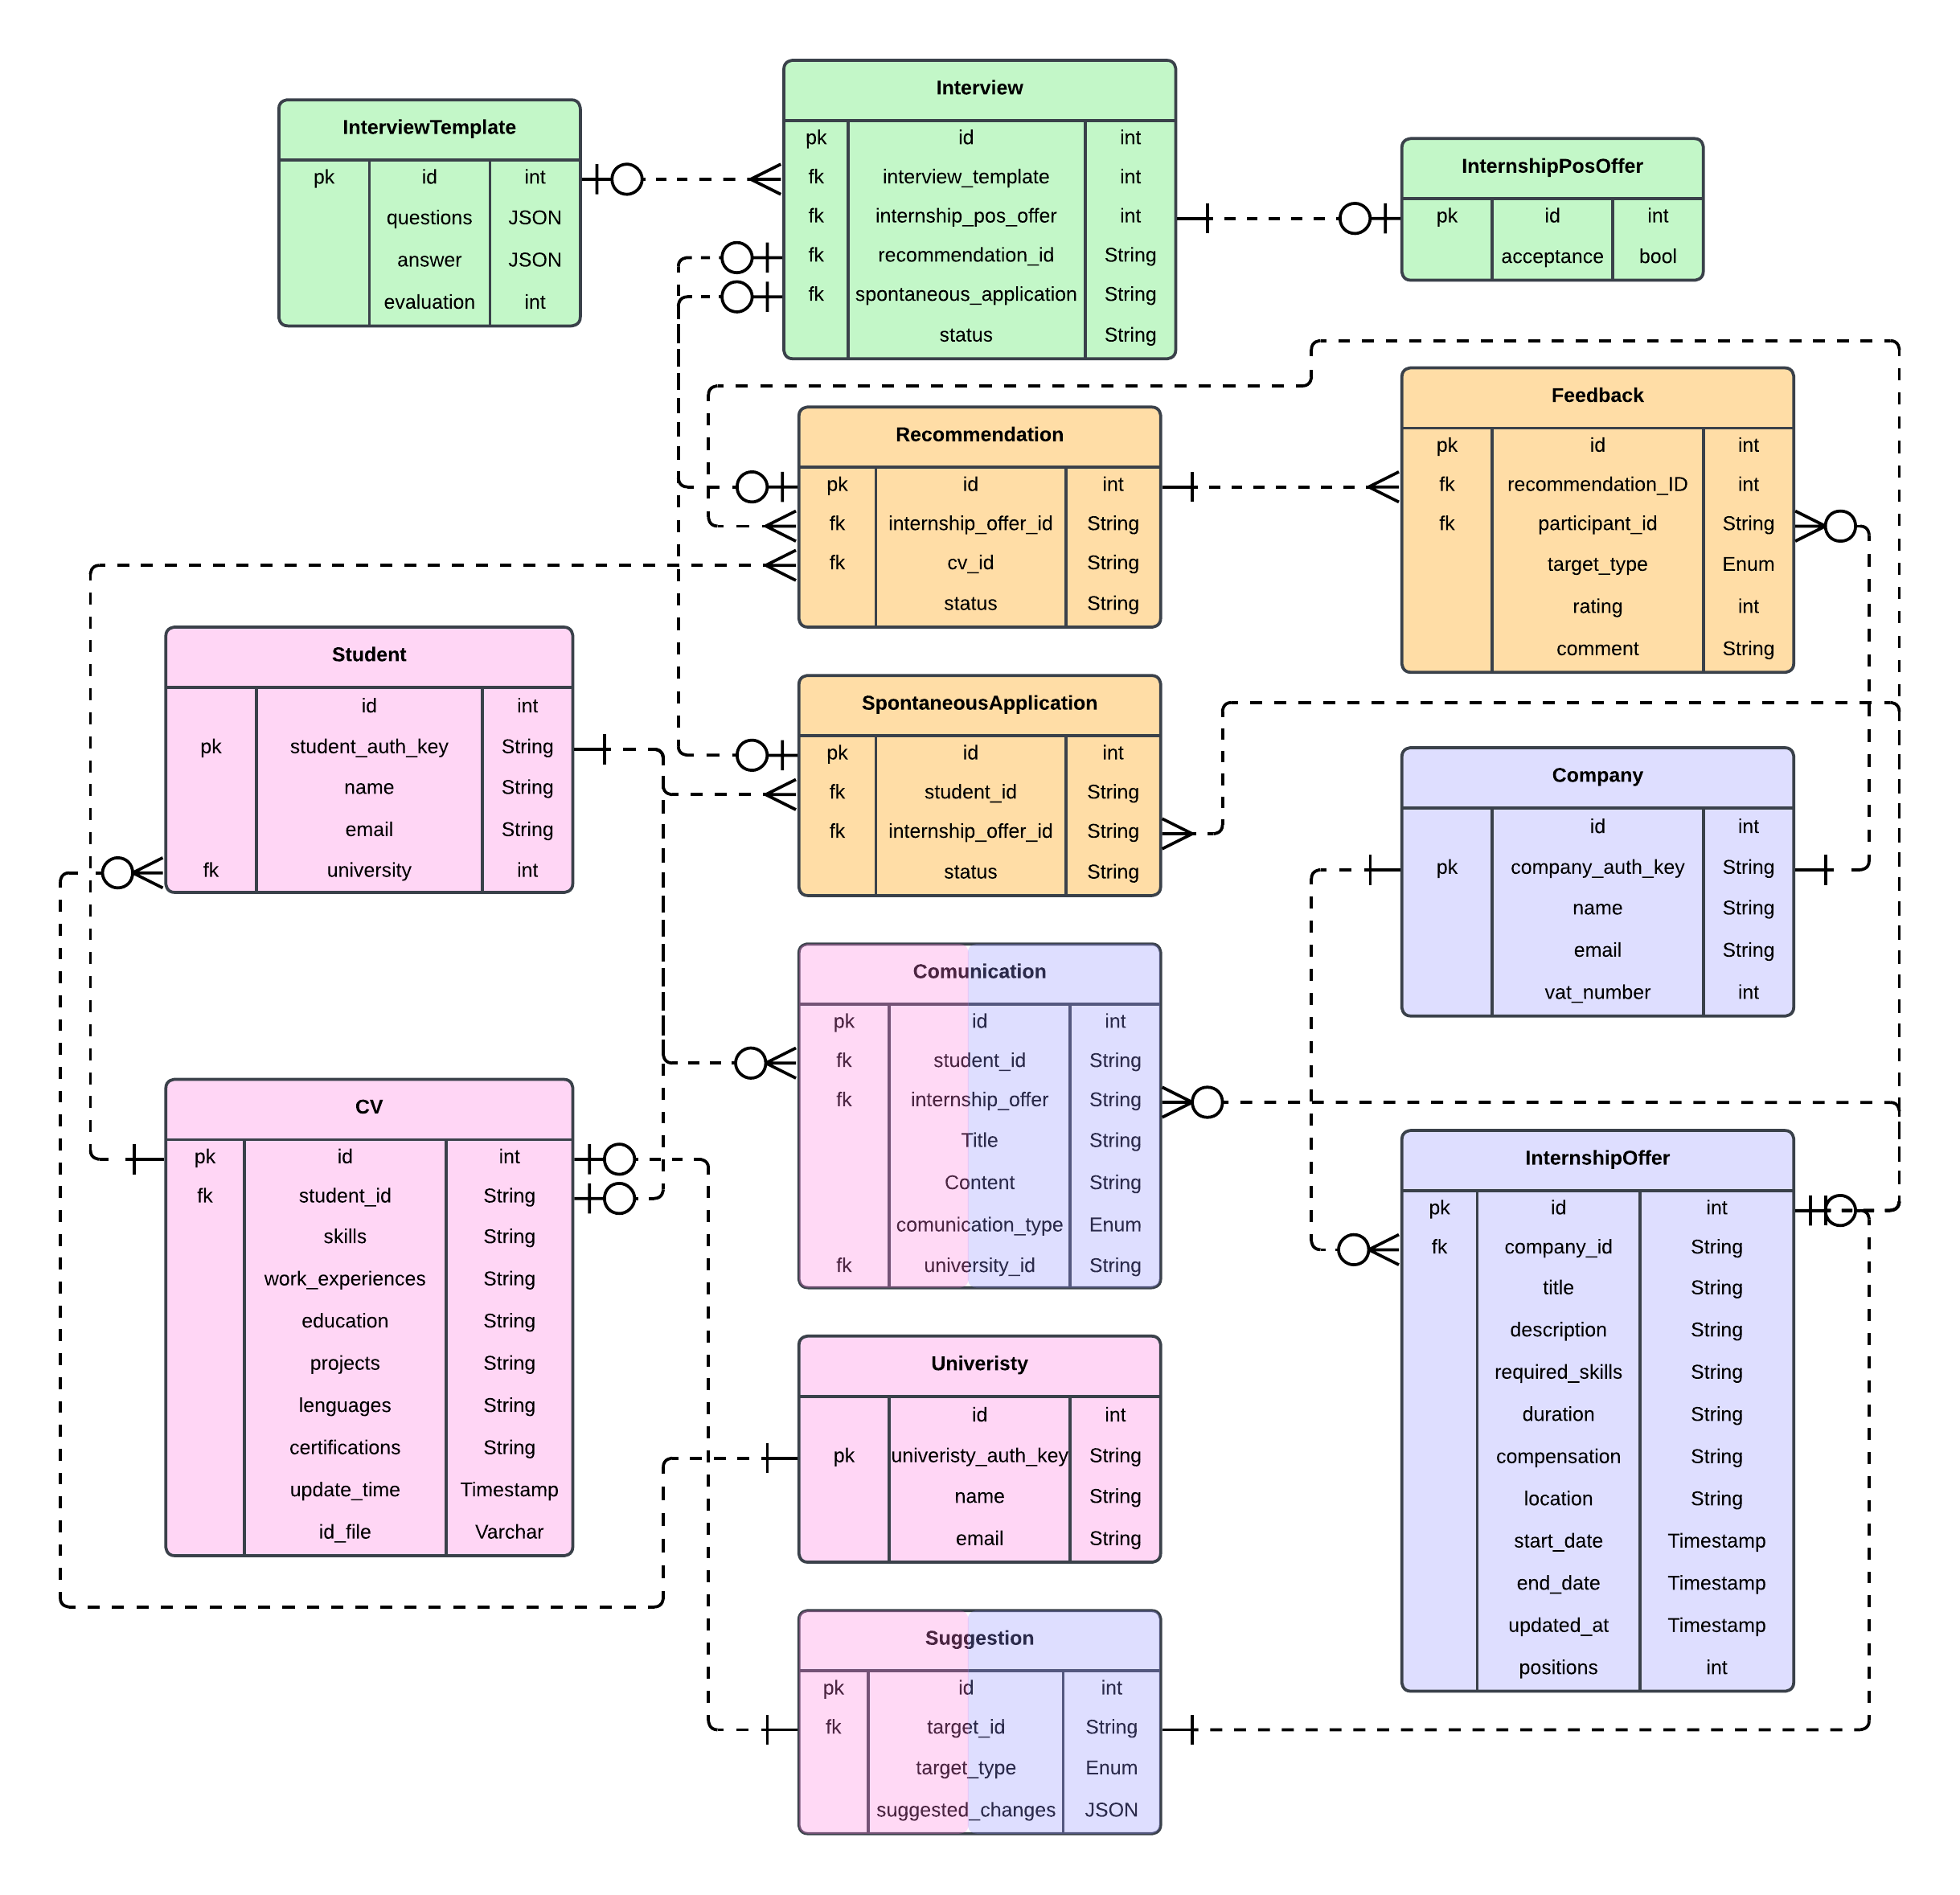
\includegraphics[width=\textwidth]{Latex/Images/DD/DatabaseSchema.png}
        \caption{Platform Database Schema}
        \label{fig:DBschema}
    \end{figure}
    \noindent Here we have the initial idea of the database structure, representing the main entities and their relationships as seen in the sequence diagram. This structure is subject to change as the development of the platform progresses and the need for new entities or relationships arises. Please note that we have not included the Notification DBMS in this diagram, as it is a separate entity from the Platform DBMS and is used exclusively by the Notification Manager. Moreover, the type used in each entity field is not specified according to a strict DBMS standard , instead more general and descriptive types, such as String, JSON, and Enum, have been used intentionally to better convey the concept and structure of the data, making it easier to understand the purpose of each field.
\subsubsection*{Notification Handling}
    Notifications of all type, both in-app and push, are handled by the Notification Manager component who is responsible to send notifications and sign-up mail confirmation to all users of the platform. This component acts both as an adapter for external push notification and email service providers and as a controller for in-app notification fetch requests. The Notification Manager is designed to do this by providing a simple interface \textit{sendNotification} that can be called to send a notification to one or more users. This is done to hide the complexity of the underlying notification system, show in sequence diagrams Sequence diagram \textit{(fig:\ref{fig:sendnotification}) Send Notification} and Sequence Diagram \textit{(fig:\ref{fig:requestdevicetoken}) RequestDeviceToken}.\\ 
    Due to the nature of this component and the high level of work it has to do, we expect it to be one of the first to be exported to its own container in the future to handle scalability concerns effectively. By decoupling the Notification Manager into its own container, the platform can better allocate resources to this high-demand service, ensuring consistent performance even under heavy load. This is why the Notification Manager in the Architecture Components Diagram \textit{(fig:\ref{fig:Components})} is represented as a separate entity from the other components, having its own interface and DB, even though it could be considered part of the Platform Logic.
\subsubsection*{Authentication and Validation}
    The user authentication process is handled by the Authenticator service, which is responsible for validating user credentials and generating tokens for authenticated users. The reason behind the use of a token-based authentication system is done because we want to limit the number of times a user has to enter their credentials while ensuring that only logged-in users can interact with \textit{private} API call. \\
    The token is generated by the Authenticator service and is stored in the Presentation layer after the user login, and it is sent every time a private request is made. The token is validated by the Authenticator service for every request, look at the Sequence Diagram \textit{(fig:\ref{fig:authentication})Authentication}, validating and refreshing the token or requesting a new login by the user, ensuring that only recent authenticated users can access the platform's functionalities. 
\subsubsection{Scalability}
    The S\&C platform is designed from the beginning to be scalable, meaning that it can handle an increasing number of users and requests without compromising performance. This is achieved through the use of a microservices architecture, which allows the platform to be divided into smaller, more manageable services that can be independently scaled as needed. Each service can be deployed in its own container, which can be easily replicated to handle additional load. This ensures that the platform can scale horizontally by adding more containers to distribute the load across multiple instances of the service. Additionally, the use of a Stateless RESTful API ensures that each request is independent and does not rely on or maintain context from previous requests, allowing the platform to scale more easily and reliably without the need for complex session management.

